\documentclass[journal,twoside]{IEEEtran}
% Draft LaTeX rendering of the identifiability manuscript (IEEE-TCI target).
% Converted from paper_draft/MANUSCRIPT_DRAFT.md + APPENDICES.md at commit c15244c2.

\usepackage[T1]{fontenc}
\usepackage[utf8]{inputenc}
\usepackage{amsmath,amssymb,amsfonts,mathtools}
\usepackage{bm}
\usepackage{graphicx}
\usepackage{booktabs}
\usepackage{array}
\usepackage{enumitem}
\usepackage[colorlinks=true,linkcolor=blue,citecolor=blue,urlcolor=blue]{hyperref}
\usepackage{xcolor}
\usepackage{float}

\graphicspath{{figs/}}

% ---- lightweight named-theorem style (labels are manual: Theorem A, A', B, ...) ----
\newenvironment{namedthm}[1]{\par\medskip\noindent\textbf{#1.}\itshape\ }{\par\medskip}
\newenvironment{nameddef}[1]{\par\medskip\noindent\textbf{#1.}\ }{\par\medskip}
% remark/status blocks
\newenvironment{statusblock}{\par\smallskip\noindent\small}{\par\smallskip}
% conventions box
\newcommand{\conv}[1]{\textbf{#1}}

% ---- shorthand macros used throughout ----
\newcommand{\Keff}{K_{\mathrm{eff}}}
\newcommand{\Kinf}{K_{\infty}}
\newcommand{\rhopair}{\rho_{\mathrm{pair}}}
\newcommand{\rhobw}{\rho_{\mathrm{bw}}}
\newcommand{\relMSE}{\mathrm{relMSE}}
\newcommand{\diag}{\operatorname{diag}}
\newcommand{\rank}{\operatorname{rank}}
\newcommand{\tr}{\operatorname{tr}}
\newcommand{\Cov}{\operatorname{Cov}}
\newcommand{\Var}{\operatorname{Var}}
\newcommand{\E}{\mathbb{E}}
\newcommand{\R}{\mathbb{R}}
\newcommand{\Prob}{\mathbb{P}}

\begin{document}

\title{Identifiability by Stationarity: Blind Gain--Object Separation in Self-Calibrating Ghost Imaging}

\author{%
CHEN Yongzi\thanks{Draft rendering; author list and affiliations to be finalized before submission.}%
}

\markboth{Draft --- for internal review (rendered \today)}{Identifiability by stationarity}

\maketitle

\begin{abstract}
With known gain, an ordered orthogonal scan minimizes conditioning-driven amplification of additive noise; with unknown slow multiplicative gain and unconstrained objects, the same deterministic chronology creates an exact gain--object ambiguity. We resolve this paradox with an identifiability theory of blind gain--object separation for single-pixel (ghost) imaging, distinguishing algebraic identifiability, statistical identifiability, and estimation conditioning. Every square invertible design fails algebraically (modulo global scale); tall designs restore uniqueness generically at $N \ge K+p$ frames for a $p$-dimensional drift class. Independently, a stationarity anchor pins the relative gain statistically: once the object carrier is stationary in time, slow modulation of the record can only be gain, recovered at the minimax rate by a windowed log-domain estimator. Acquisition by the randomized Hadamard transform (SRHT, at full sampling) preserves orthogonal conditioning while supplying, under Walsh-flatness or a successful random permutation of a sufficiently spread object, the stationary or exchangeable carrier the estimator needs; an exact finite-noise relative mean-square-error identity then yields a design chart with a computable flip boundary between ordered and randomized acquisition, whose gain-known skeleton is validated on the simulation grid with no free parameters (raw-metric median agreement factor 1.04). In frame-matched simulations, raw ordered Hadamard leaves a non-decaying blind gain error of 0.94--0.99 across all averaging windows, where randomized arms reach 0.007--0.015 (medians with two-way clustered 95\% confidence intervals), and randomized Hadamard acquisition recovers $+5.45$ dB under slow drift. The acquisition rule: randomize the carrier's chronology --- make the object stop pretending to be time.
\end{abstract}

\begin{IEEEkeywords}
ghost imaging; single-pixel imaging; blind calibration; identifiability; bilinear inverse problems
\end{IEEEkeywords}


\section{Introduction}

Single-pixel (ghost) imaging \cite{Pittman1995PRA,Bennink2002PRL,Shapiro2008PRA,Bromberg2009PRA} has become the method of choice for imaging through media that defeat conventional cameras \cite{Bina2013PRL,Cheng2009OE}: turbid water, fog, dynamic scattering media \cite{PengChen2024APL}, complex channels around corners \cite{PengXiaoChen2025OE}. The instrument is disarmingly simple --- structured illumination patterns and a bucket detector \cite{Duarte2008SPM,Edgar2019NatPhoton} --- and the textbook design instinct is equally simple: use an ordered orthogonal basis. A Hadamard scan acquires one transform coefficient per frame \cite{Zhang2017OE,Yu2019Sensors}, the measurement matrix is perfectly conditioned, and an exact inverse waits at the end of the acquisition; against additive noise this is provably the safe choice.

Dynamic media break this instinct in a specific, instructive way. A time-varying channel multiplies the bucket record by a slowly drifting gain: the $n$-th measurement is $R_n = a_n B_n$, with $B_n$ the object-dependent bucket coefficient and $a_n > 0$ an unknown per-frame gain whose log-gain $\ell_n = \log a_n$ is confined to a slow-drift class $S$ of dimension $p$. Ghost imaging through dynamic and complex scattering media \cite{PengChen2024APL} shows a self-calibrating scheme built on \emph{random} illumination with supervised correction of dynamic scaling factors succeeding where ordered scans fail, and optical wireless transmission around corners \cite{PengXiaoChen2025OE} relies on the same random-pattern robustness. Read naively, this is a puzzle: the ordered Hadamard scan is the better-conditioned instrument, yet randomness --- usually a concession, not a feature --- wins; it is desirable to determine when, and by what mechanism, a drifting gain becomes blindly separable at all.

The resolution is that under gain drift the ordering itself becomes the liability. An ordered scan sorts the object's transform coefficients into a smooth sequence in acquisition time, so the object acquires a \emph{temporal signature}: a slow gain trace and a slow coefficient trace cast the same shadow on the one-dimensional bucket record, and no estimator can tell them apart from that record alone. Hadamard is not defeated by randomness; it is defeated by chronology. This confounding is not an artifact of any particular correction algorithm but a genuine algebraic ambiguity --- for a square unconstrained design, \emph{any} invertible pattern matrix can absorb a nonconstant gain into a perfectly valid alternative object (Theorem~A). Conversely, random carriers escape it statistically when their log-carrier window means are time-homogeneous and concentrate as condition ($\star$): slow gain is then the only persistent local modulation, and relative gain is recovered up to the unavoidable global scale (Theorem~B). Self-calibration is thus a property one can \emph{design into acquisition time}, with price, rates, and failure boundaries computable in advance.

We develop that observation into a quantitative identifiability theory; the contributions are:

\begin{enumerate}[leftmargin=*,itemsep=1pt,topsep=2pt]
\item \textbf{A three-notion identifiability framework} for the bilinear model $R_n = a_n B_n$, separating exact-algebraic identifiability, statistical (asymptotic) identifiability, and estimation conditioning. Within it, the square-design obstruction (Theorem~A) and the tall-design thresholds (Theorem~A$'$) are proved for every fixed drift class $S$ containing the constants: generic exact identifiability at $N \ge K + p$ for almost every design--object pair, uniform identifiability over every nonvanishing-carrier object at $N \ge 2K + p - 1$, and a generic local threshold at $N = K + p - 1$ that is an if-and-only-if for $K \ge 2$, with genuine positive-dimensional alias families below it (Secs.~4, 9). This is distinct from generic bilinear-injectivity results \cite{KechKrahmer1603.07316,LiLeeBresler1501.06120,AhmedRechtRomberg1211.5608,ChoudharyMitra1402.2637,KuengRauhutTerstiege1410.6913}: the operator here is a diagonal-row map, and the anchor is temporal, not structural.

\item \textbf{The stationarity anchor (Theorem~B)} and its consistency condition ($\star$): under explicit triangular-array bias and window-variance conditions, random carriers pin the relative gain statistically. A separate \emph{oracle-known-carrier} calibrated soft-log theorem covers the photon-limited case, with a conditional $1/(W\bar\lambda)$ law in the locally-flat-gain regime. The blind high-count and known-carrier low-photon experiments are distinct.

\item \textbf{A synthesis, not a trade-off:} randomized Hadamard (SRHT) designs retain orthogonal conditioning while randomizing the temporal carrier. Pixel signs and a pixel permutation control ensemble covariance through an exact Walsh-domain criterion; a separate random acquisition order supplies finite-population exchangeability. A conditioned draw is deterministic, so these two randomization semantics are not conflated.

\item \textbf{An exact finite-noise reconstruction bridge} (Theorem~1) expressing raw relative MSE for any fixed linear reconstructor through a leverage functional $B_L$, under explicit exogenous-gain hypotheses. Physical nonnegative Poisson measurements, signed coefficient-domain noise, and complementary-pair noise are kept as distinct specializations \cite{Ferri2010PRL,Sun2012OE}.

\item \textbf{A finite-$N$ flip diagnostic} $\rho^*$ in $\rho_{\mathrm{pair}}$ (Prop.~3): its gain-known true-$S_1$ skeleton is validated without fitted parameters; the production normalization and same-record blind arm are reported separately as robustness and conditional-proxy checks.
\end{enumerate}

All results are theoretical, supported by numerical evidence; no hardware validation is reported. Identifiability near $N = K + p$ is a uniqueness statement, not a conditioning guarantee, and random square designs remain algebraically non-identifiable --- their advantage is statistical. The organizing idea is the distilled paradox: one makes the gain observable not by measuring it directly, but by making the object stop pretending to be time.

Figure~1 maps ordered-Hadamard, iid-random, tall-random, and SRHT designs on the resulting conditioning-versus-identifiability axes; Sec.~10 collects the design rules, scope, and outlook.

\begin{figure}[!t]
\centering
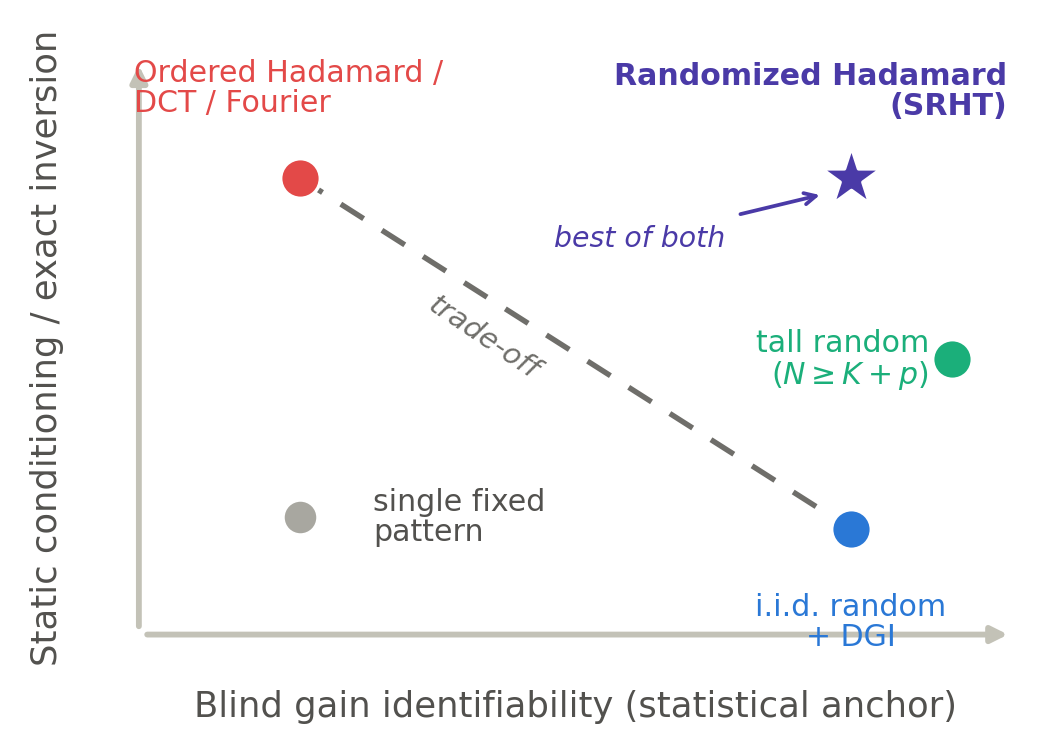
\includegraphics[width=0.55\columnwidth]{fig1_conceptmap.png}
\caption{Two-axis map of inversion conditioning against blind identifiability. Ordered orthogonal scans (Hadamard/DCT/Fourier) are well-conditioned yet blindly non-identifiable; i.i.d.-random (DGI) acquisition buys the statistical anchor at the cost of conditioning; a single fixed pattern (grey) has neither; tall random designs ($N\ge K+p$) restore exact identifiability modulo scale for almost every design--object pair (Theorem~A$'$(ii)); SRHT (star) retains orthogonal conditioning while randomizing the temporal carrier. The dashed diagonal marks the apparent trade-off the SRHT synthesis dissolves (Secs.~4 and 5).}
\end{figure}

\section{Problem setup and three notions of identifiability}

In a single-pixel (bucket-detection) acquisition of $N$ frames, frame $n$ illuminates a static object $T \in \mathbb{R}^K$ with a programmed pattern $m_n \in \mathbb{R}^K$, producing the ideal bucket value $B_n = m_n^{\mathsf T} T$ --- the \emph{object carrier}. The record is corrupted by a slowly drifting multiplicative gain (source power, detector responsivity, coupling):

\[
R_n \;=\; a_n B_n, \qquad a_n = e^{\ell_n} > 0 ,
\]

where $a_n$ is the unknown per-frame gain and the log-gain trajectory $\ell = (\ell_1,\dots,\ell_N)$ is confined to a \emph{drift class} $S \subset \mathbb{R}^N$, $p = \dim S$, always containing the constants. The constant direction is a pure gauge: $(a, T) \mapsto (c\,a,\; T/c)$ leaves every $R_n$ invariant, so all statements are up to a global scale. For physically slow drift, $S$ is a low-pass (Fourier) space of normalized bandwidth $\rho_{\mathrm{bw}}$, $p \approx \rho_{\mathrm{bw}} N$ (not to be confused with the adjacent-pair decorrelation $\rho_{\mathrm{pair}}$ of Sec.~8). The blind problem --- recover $(a, T)$ from $\{R_n\}$ alone --- is bilinear, and asking whether it is ``solvable'' turns out to be three distinct questions; separating them is itself a contribution of this paper.

\begin{nameddef}{Conventions (fixed throughout)}
$K$ --- pixels; $T\in\mathbb{R}^K$ the object, nonnegative unless stated; $N$ --- frames; $S$ --- linear log-gain drift class, \textbf{always containing the constants}, $p=\dim S$. \textbf{All} identifiability statements are modulo the gauge $(a,T)\mapsto(c\,a,\,T/c)$, fixed by centering the log-gain. Theorem~1 and Prop.~3 use raw relative MSE; least-squares scale-aligned MSE is a separately labeled image-quality metric. \emph{Local-differential}, \emph{generic-exact}, and \emph{uniform-exact} identifiability are distinct properties with distinct thresholds (Theorem~A$'$); none implies conditioning. $\rho_{\mathrm{bw}}$ --- normalized gain bandwidth, $p\approx\rho_{\mathrm{bw}}N$ (Sec.~4); $\rho_{\mathrm{pair}}$ --- adjacent-pair gain decorrelation (Sec.~8); related but not equal. The object functionals $K_{\mathrm{eff}}$, $K_\infty$, $K_4$ and pipeline constants $C_0$, $D_H$, $B_L$ are defined at first use (Prop.~1, Secs.~6--8); a consolidated notation table appears in Supplementary Material S5.
\end{nameddef}

Pattern entries $m_n$ may be signed (Hadamard) or nonnegative (speckle); where signed coefficients appear as carriers, the Sec.~5 bucket conventions specify their physical realization.

\noindent\textbf{Algebraic identifiability.} Does the noiseless record determine $(a,T)$ up to gauge, or does some other pair with $\ell' - \ell \in S$ nonconstant reproduce the data exactly --- a finite-sample, deterministic question about collisions $MT = D_s M T'$? Section~4 shows that every square invertible design, however well-conditioned, fails it, and that overdetermination restores it generically at $N \ge K + p$.

\noindent\textbf{Statistical identifiability.} Under random pattern ensembles a weaker but operationally decisive property becomes available: if the carrier is time-homogeneous and its log-carrier window means concentrate according to ($\star$), then any persistent slow modulation of those averages is attributable to gain, and the relative gain is recoverable even where exact algebraic separation is impossible. Stationarity alone is not sufficient without the window-variance condition. This stationarity anchor (Sec.~5, Theorem~B) is the mechanism the field's empirical successes have been implicitly exploiting.

\noindent\textbf{Estimation conditioning.} Uniqueness is not accuracy: even when one of the first two notions holds, the finite-noise error of a concrete estimator is governed by conditioning quantities --- the window $W$, the residual-gain variance $v$, the leverage $B_L$ --- quantified in Secs.~6 and 8. Identifiability at the threshold $N = K + p$ says nothing about stability there.

Much of the confusion surrounding blind gain correction stems from conflating these three notions: judging a scheme by the visual quality of a blindly corrected reconstruction entangles algebraic ambiguity, the statistical anchor, and estimator conditioning into a single scalar --- three failures with different remedies. Figure~1 disentangles them as a two-axis map --- inversion conditioning against blind identifiability --- on which ordered Hadamard, i.i.d.-random (DGI), tall random, and SRHT acquisitions occupy visibly different corners (Secs.~4 and 5).

\section{Relation to prior work}

Gain--object separation is a bilinear inverse problem: lifting the unknowns to the rank-one array $X=aT^{\top}$, each bucket $R_n=a_n B_n$ with $B_n=m_n^{\top}T$ is a bilinear form in the object $T$ and the gain trace $a$. This places the question inside a mature literature on bilinear identifiability; we state what it settles and what it leaves open for the diagonal-gain geometry.

The sharpest injectivity counts for lifted bilinear maps are Kech--Krahmer's optimal conditions for generic identifiability \cite{KechKrahmer1603.07316}, requiring on the order of $2(n_1+n_2)-4$ generic rank-one measurements. These counts do not transfer here: the operator $L_M(X)_n=a_n\,m_n^{\top}T$ is a \emph{diagonal-row} map, not a generic rank-one measurement, and the relevant question is the intersection geometry of the object subspace with its gain-modulated copy, $\,U\cap D_sU$. Choudhary--Mitra's scaling laws \cite{ChoudharyMitra1402.2637} are the closest in spirit to our Theorem~A: their rank-two nullspace obstruction is exactly the mechanism by which a square unconstrained design absorbs a nonconstant gain into a redefined object. Li--Lee--Bresler's unified framework \cite{LiLeeBresler1501.06120} supplies the subspace- and sparsity-constrained thresholds that our tall-design counts ($N\ge K+p$ generic, $N\ge 2K+p-1$ uniform) specialize to for the diagonal-gain model. Ahmed--Recht--Romberg \cite{AhmedRechtRomberg1211.5608} establish convex recovery for blind deconvolution under subspace priors, and Kueng--Rauhut--Terstiege \cite{KuengRauhutTerstiege1410.6913} give low-rank-from-rank-one-measurement guarantees; both are the algorithmic backdrop for our purely algebraic and statistical criteria.

On the imaging side, single-pixel practice has long weighed ordered Hadamard against random speckle for conditioning and noise, but without an identifiability account of slow multiplicative drift. Learned correction of dynamic scaling factors \cite{PengChen2024APL} and learned encoding for optical wireless links \cite{PengXiaoChen2025OE} address the same nuisance empirically; our analysis explains why their \emph{static-correction ceiling} --- the error floor left by any time-independent correction applied to a drifting record --- is the honest bound, and when a drifting gain becomes blindly separable at all. Blind self-calibration of sensor gains and phases has a long history outside imaging --- eigenstructure methods \cite{WeissFriedlander1990}, blind sensor-network calibration \cite{Balzano2007IPSN}, biconvex compressive self-calibration \cite{LingStrohmer2015} --- and Balzano--Nowak similarly find gains recoverable under mild oversampling, which our threshold $N\ge K+p$ makes exact for the diagonal bilinear model. On the acquisition-design side, pink-noise speckle \cite{Nie2021PRA} and sparse Hadamard sequencing \cite{Han2025OE} optimize the pattern set directly but target additive-noise robustness, not multiplicative-drift identifiability.

Against this background the contribution is specific: we do not add to generic bilinear injectivity, settled above. New is the temporal-statistical mechanism --- relative-gain identifiability secured by making the carrier stationary (Theorem~B), a general mixing-law upper bound together with a matching fixed-iid-Gaussian interior benchmark, the ordered-orthogonal confounding failure mode it repairs, the SRHT synthesis, and the finite-noise bridge that renders the phase diagram quantitative. The novelty is the stationarity anchor, not bilinear injectivity per se.

\section{The algebraic obstruction and when oversampling cures it}

The paradox of Sec.~1 is not an estimator artifact. Stack $N=K$ frames of the noiseless record $R_n = a_n B_n$ into an invertible square design $M$: the multiplicative drift is absorbed \emph{exactly} into a relabelled object.

\begin{namedthm}{Theorem A (square non-identifiability)}
For any invertible $M\in\mathbb R^{K\times K}$ and any gain $a=(a_n)$ nonconstant on the support of the carrier $MT$, there exists a distinct object $T'\neq cT$ producing the identical bucket record: $\operatorname{diag}(a)MT = M T'$ with $T'=M^{-1}\operatorname{diag}(a)MT$. Gain--object separation is unidentifiable up to the global-scale gauge $a\mapsto ca,\ T\mapsto T/c$. (Proof: Appendix~A.)
\end{namedthm}

The object is a barcode printed onto time and the drift a smudge across it; when the barcode carries slow structure, the smudge can be \emph{reread as a different barcode} rather than dismissed as blur --- a genuine orbit of the bilinear map, for \emph{every} invertible design. Two corollaries sharpen the trap (full statements and proofs: Appendix~A). \emph{Corollary~1 (slowness does not help):} restricting $\ell\in S$ to a slow drift class does not restore identifiability at $N=K$ --- for any nonconstant $s\in S$ the alternative pair $\big(\ell-s,\; T'=M^{-1}\operatorname{diag}(e^{s})MT\big)$ explains the record exactly. \emph{Corollary~2 (known support zeros):} nonnegativity alone does not break the orbit. For fixed known support, a displayed quotient-Jacobian full-rank condition is equivalent to \emph{differential} identifiability and is sufficient for ordinary local identifiability; the exact ordinary-local condition is isolation of the nonlinear gauge-fixed support zero. The count $K_0\ge p-1$ is necessary only for that full-rank test and is not by itself an ordinary-identifiability theorem. This qualification does not affect Theorem~A$'$(i) below.

The first escape is overdetermination. For a tall design $M\in\mathbb R^{N\times K}$, $N>K$, a collision $\operatorname{diag}(e^{s'})MT'=\operatorname{diag}(e^{s})MT$ pits $K+p$ unknowns against $N$ equations, suggesting uniqueness once $N\ge K+p$; the following theorem turns this count into proved sufficiency thresholds, for every fixed drift class $S\ni\mathbf 1$, at the price of almost-everywhere quantifiers with explicit Lebesgue-null exceptional sets.

\begin{namedthm}{Theorem A$'$ (proved tall-design identifiability results)}
Let $K\ge1$, $N\ge K$, and let $S\le\mathbb R^N$ be a fixed, known linear subspace of dimension $p\ge2$ with $\mathbf 1\in S$. For $M\in\mathbb R^{N\times K}$ define $\Phi_M(T,s)=D_{e^{s}}MT$ and $\mathcal U_M=\{T\in\mathbb R^K:(MT)_n\neq0\ \text{for every } n\}$. Parameters are identified modulo the positive global-scale gauge $(T,s)\sim(cT,\,s-\log c\,\mathbf 1)$, $c>0$.

\emph{(i) (Generic local threshold and genuine failure below it, $K\ge2$.)} There is a Lebesgue-null set $E_{\mathrm{loc}}\subset\mathbb R^{N\times K}\times\mathbb R^K$ such that for every $(M,T)\notin E_{\mathrm{loc}}$ with $T\in\mathcal U_M$ and every $s\in S$: $\operatorname{rank}D\Phi_M(T,s)=\min\{N,K+p-1\}$. Consequently $(T,s)$ is locally identifiable modulo gauge iff $N\ge K+p-1$. If $N\le K+p-2$ then a gauge-normalized neighborhood of $(T,s)$ contains a real-analytic manifold of exact aliases of dimension $K+p-N-1\ge1$, and every other sufficiently nearby point of it is gauge-inequivalent.

\emph{(ii) (Generic exact-identifiability sufficiency.)} If $N\ge K+p$, there is a Lebesgue-null set $E_{\mathrm{gen}}\subset\mathbb R^{N\times K}\times\mathbb R^K$ such that for every $(M,T)\notin E_{\mathrm{gen}}$ and every $s\in S$: $D_{e^{s'}}MT'=D_{e^{s}}MT$ with $(T',s')\in\mathbb R^K\times S$ implies $T'=cT$, $s'=s-\log c\,\mathbf 1$ for a unique $c>0$. Exact identifiability holds simultaneously for every possible true drift $s\in S$. This statement is \textbf{not} uniform over all objects for one fixed $M$.

\emph{(iii) (Uniform exact-identifiability sufficiency on the nonvanishing-carrier set.)} If $N\ge2K+p-1$, there is a Lebesgue-null set $E_{\mathrm{unif}}\subset\mathbb R^{N\times K}$ such that for every $M\notin E_{\mathrm{unif}}$, every $T\in\mathcal U_M$, every $s\in S$, and every $(T',s')\in\mathbb R^K\times S$: $D_{e^{s'}}MT'=D_{e^{s}}MT$ implies $T'=cT$, $s'=s-\log c\,\mathbf 1$ for a unique $c>0$. The same generic design works simultaneously for all nonvanishing-carrier objects and all true drifts in $S$.

\emph{(iv) (Degenerate one-dimensional object stratum.)} If $K=1$ then for every $M$ and every $T\in\mathcal U_M$ and every $s\in S$, the pair $(T,s)$ is globally identifiable modulo gauge, for every admissible $N$. Neither $N\ge K+p$ nor $N\ge2K+p-1$ is necessary when $K=1$.

(Proof: Appendix~B.)
\end{namedthm}

\noindent\textbf{Sharpness status.} Parts (ii) and (iii) are sufficient conditions, not proved if-and-only-if thresholds. For $K\ge2$, the below-wall part of (i) proves generic exact failure whenever $N\le K+p-2$. The remaining necessity assertion for the $K+p$ bound is the boundary case $N=K+p-1$: dimension counting predicts nonlocal aliases there, but dominance of the bad-pair projection has not been proved. Likewise, dimension counting predicts that a generic design fails uniform identifiability for some object when $N\le2K+p-2$, but this necessity direction has not been proved in the intermediate regime. Thus $K+p$ and $2K+p-1$ are conjecturally sharp for $K\ge2$ under generic/nondegenerate drift geometry, not universal sharp thresholds for every fixed $S$. The $K=1$ stratum explicitly rules out any universal necessity claim.

The proof is a parametric-transversality argument (Appendix~B): a rowwise perturbation of $M$ acts as a global witness on a collision incidence manifold, and no genericity of the drift family is invoked, so the statements hold verbatim for the physical Fourier low-pass class $S_{\mathrm{LP}}$ and any other fixed drift convention containing the constants. Empirically, the $K=64$ and $K=128$ threshold scans of Sec.~9 (Fig.~6) show an exact $0\%\to100\%$ rank transition at $N=K+p-1$ across all five drift dimensions at both object sizes (3250 cells, no exceptions) --- a direct verification of the generic local rank wall of part (i). Part (ii) asserts \emph{generic exact finite-sample identifiability}, not a conditioning bound and not an algorithmic recovery guarantee; stability near the thresholds is the separate third notion of Sec.~2, quantified in Secs.~6 and 8.

The picture is a dichotomy. When $N\ge K+p$, overdetermination \emph{alone} separates gain from object for almost every design--object pair --- no statistical mechanism is logically needed, though randomization still buys stable conditioning (Fig.~1). When $K<N\le K+p-2$, generic local and exact identifiability fail through positive-dimensional nearby alias families; at $N=K+p-1$, local identifiability holds generically, while failure of global exact identifiability remains a dimension-count prediction. In that under-resourced window some additional information is required --- the stationarity anchor of Sec.~5 and support/sparsity priors are examples, not an exhaustive list. The regimes meet through the drift bandwidth: a gain occupying a fraction $\rho_{\mathrm{bw}}$ of the frame band spans $p\approx \rho_{\mathrm{bw}}N$ low-pass modes, so $N\ge K+p$ reads as $N \gtrsim K/(1-\rho_{\mathrm{bw}})$. Slow drift ($\rho_{\mathrm{bw}}\ll1$) is cured by modest oversampling; as $\rho_{\mathrm{bw}}\to1$, $p\to N$ and blind algebraic separation is impossible for \emph{any} $N$, forcing some non-algebraic information source.

\section{Statistical identifiability: the stationarity anchor}

Section~4 bought identifiability with surplus rows; this section develops a second, logically distinct escape that operates even at fixed $N$ and explains \emph{why} randomized acquisition self-calibrates while ordered acquisition does not. A drifting gain is a boat carried by a slow current, and the bucket record is our only view of the water: if the waves change character with position --- as the ordered Hadamard coefficient sequence does --- we cannot tell the current from the coastline; if the waves are \emph{statistically identical everywhere}, any slow modulation of the record has exactly one explanation. Local averaging then pins the \emph{relative} drift, the absolute scale remaining gauged away. This intuition, and nothing stronger, is what the results below formalize.

The log-domain record can be described by $Y_n=\log R_n=\ell_n+\log B_n$. The anchor requirement is a condition on the carrier alone:

\begin{nameddef}{Condition ($\star$) (stationary carrier, quantitative form)}
There is a scalar $m_T$ --- depending on the object but not on time, and absorbed by the global-scale gauge --- such that the windowed carrier averages over windows $W_n$ of length $W$ satisfy
\[
\begin{gathered}
\max_n \Big| W^{-1}\!\!\sum_{k\in W_n}\!\log B_k \;-\; m_T \Big| \;\longrightarrow\; 0\\
\text{in probability as } W\to\infty,\ W/N\to 0 .
\end{gathered}
\]
Condition ($\star$) and Theorem~B presuppose a positive carrier with an integrable log on the analyzed record, typically enforced by a physical positivity/offset margin. Photon-counting records with zeros are treated separately by the oracle-known-carrier soft-log Theorem~C; that result is not a blind extension of ($\star$).
\end{nameddef}

The criterion is deliberately \emph{uniform} (a maximum over all window locations); the pointwise-to-uniform upgrade typically costs a $\log N$ refinement (the $\delta\mapsto\delta/N$ step of Appendix~C).

I.i.d. random illumination satisfies ($\star$) under the stated log-tail control and a window sequence large enough to pay the $\log N$ uniformity cost; iid alone gives only the pointwise law without that scaling. A uniform acquisition-order permutation $P_{\mathrm{row}}$ makes the sequence finite-population exchangeable over that randomization draw, whereas a shared pixel permutation $P_{\mathrm{col}}$ controls ensemble covariance but is not joint row exchangeability. After conditioning on either draw the record is deterministic, and a particular realization can fail the window criterion. For the i.i.d. case:

\begin{namedthm}{Proposition 1 (random-basis carrier)}
For i.i.d. random patterns with pixel mean $\mu_I$ and standard deviation $\sigma_I$, the carrier $\{B_n\}$ is white and strictly stationary, and the object enters its first two moments only through the scalars $S_1=\sum_j T_j$ and $S_2=\sum_j T_j^2$: $\mathbb{E}B_n=\mu_I S_1$, $\operatorname{Var}B_n=\sigma_I^2 S_2$, hence $\mathrm{CV}_B=(\sigma_I/\mu_I)/\sqrt{K_{\mathrm{eff}}}$ with $K_{\mathrm{eff}}=S_1^2/S_2$. The Gaussian approximation additionally requires the Lindeberg-type spikiness condition $K_\infty=S_2/\|T\|_\infty^2\to\infty$; the log-domain expansion further requires positivity, log-integrability, and the lower-tail control stated in Appendix~C. The reduction of the object to two scalars holds at the leading Gaussian/log-variance level, not exactly. Higher cumulants can depend on object shape beyond $(S_1,S_2)$: their contribution to the log mean is a time-constant gauge term, while their contribution to log variance and tails changes finite-sample rate constants. It does not create a time-varying carrier bias or invalidate consistency when ($\star$) holds. (Proof: Appendix~C.)
\end{namedthm}

Figure~2 shows the two carriers side by side: the random trace is a time-homogeneous, object-dependent noise band without an object-specific temporal envelope, whereas the ordered Hadamard trace \emph{is} the object's coefficient envelope --- the object masquerades as a temporal trend, precisely the degree of freedom a slow gain occupies, and ($\star$) fails. The condition's logical status:

\begin{namedthm}{Proposition 2 (($\star$) is an estimator criterion, not a universal one)}
Condition ($\star$) is necessary and sufficient for consistency of the stated blind windowed log estimator. It is \emph{not} an if-and-only-if condition for identifiability by all mechanisms or for every windowed correction rule: the overdetermined designs of Sec.~4 identify algebraically --- for almost every design--object pair at $N\ge K+p$, Theorem~A$'$(ii) --- without any stationarity, and conversely ($\star$) confers no exact algebraic identifiability. (Proof: Appendix~C.)
\end{namedthm}

\begin{figure*}[!t]
\centering
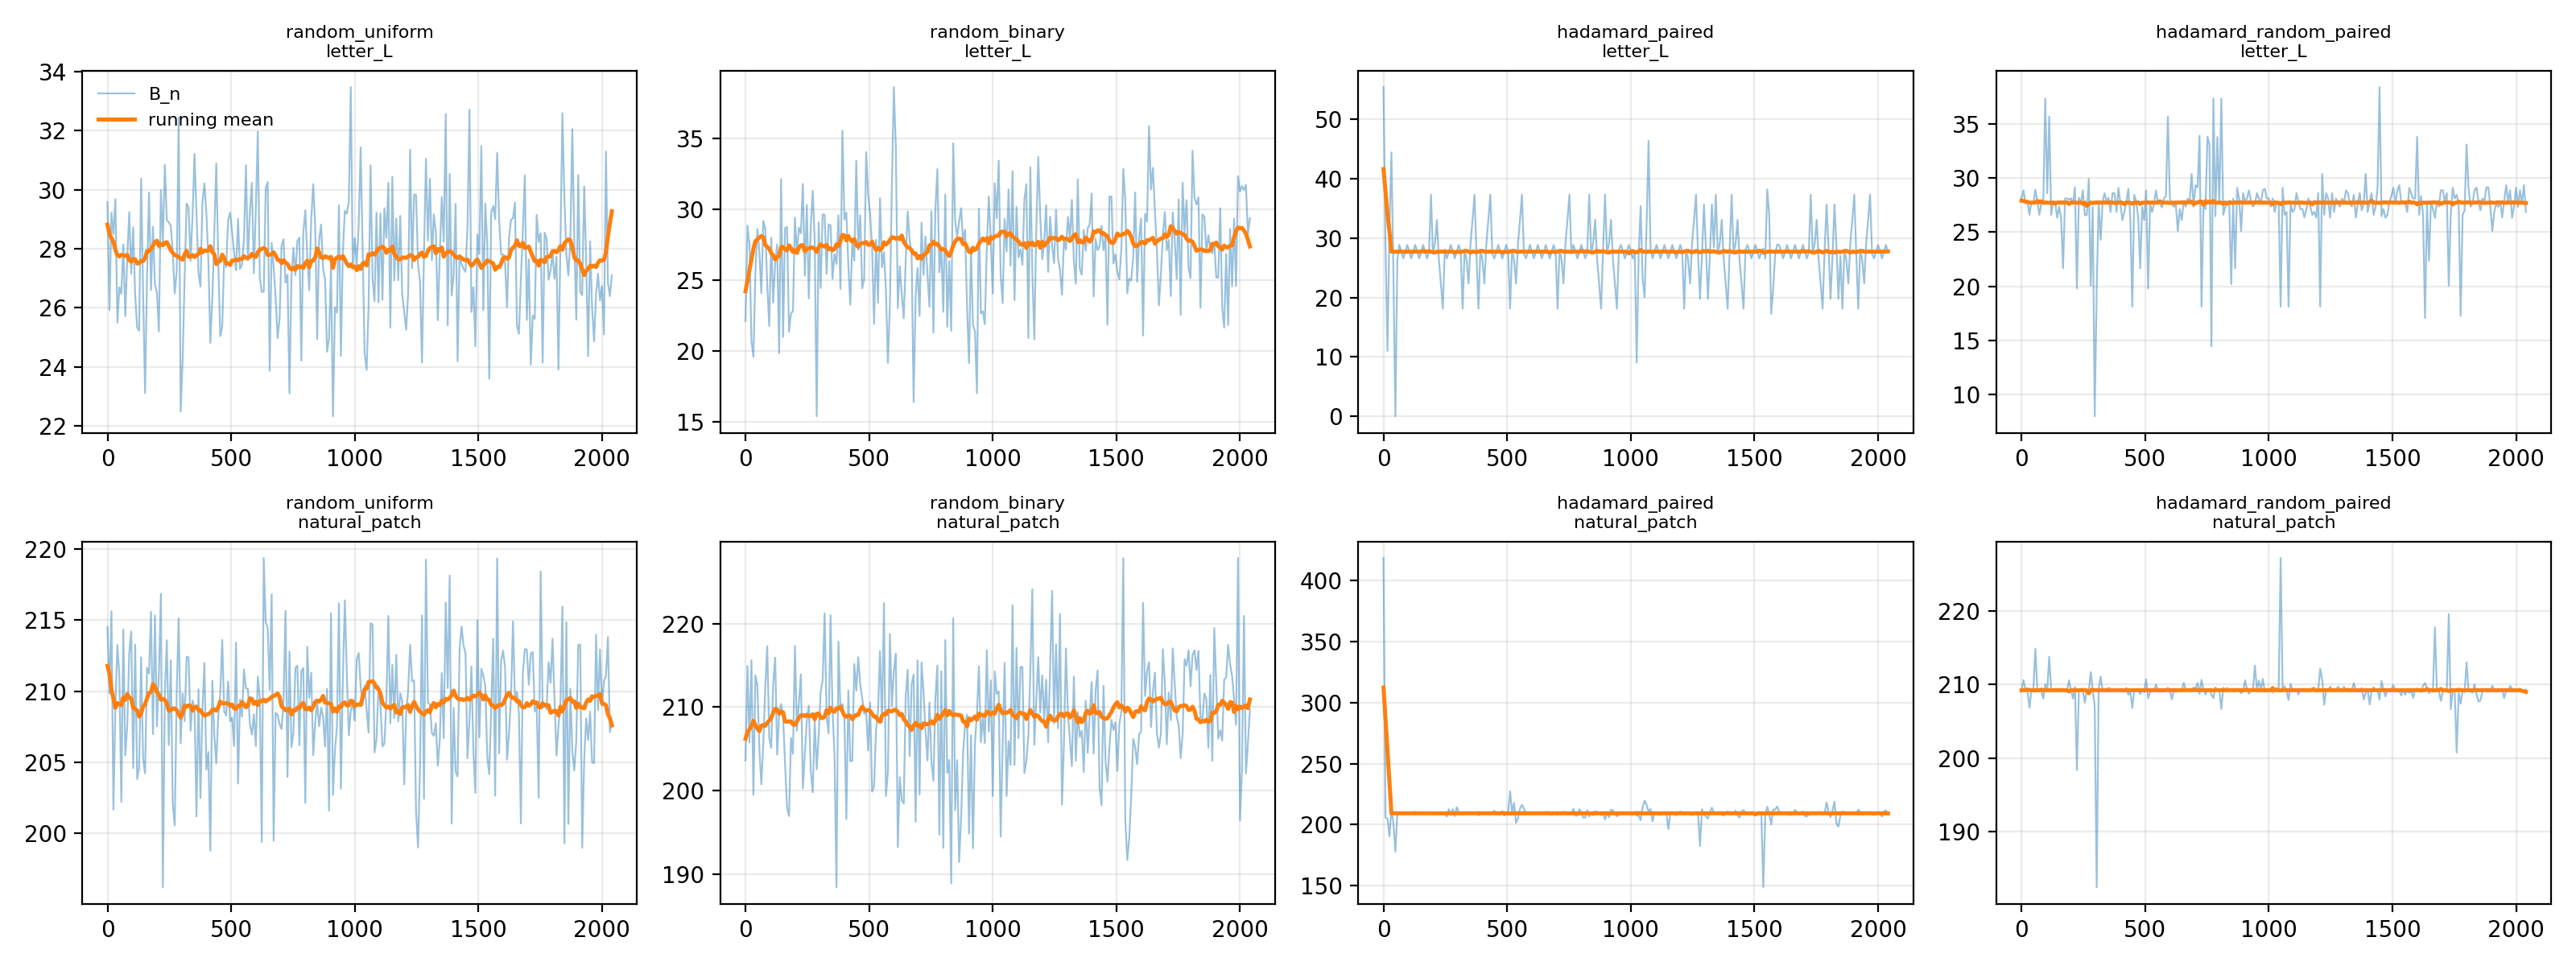
\includegraphics[width=0.50\textwidth]{fig2_carrier_traces.png}
\caption{Carrier stationarity: noiseless bucket carriers $B_n$ (thin), running means (bold), and the $\pm1$\,SD envelope for one object (digit\_0; 8192 frames, $64\times64$), before any gain is applied. (a) The i.i.d.\ random-uniform carrier is a time-homogeneous, object-dependent noise band without an object-specific temporal envelope; (b) the ordered Hadamard trace \emph{is} the object's coefficient envelope --- a deterministic, non-stationary temporal signature. Rejection counts and the Parseval invariant: Sec.~9.1.}
\end{figure*}

\noindent\textbf{Bucket conventions.} Three bucket-signal conventions coexist (full statement: Supplementary Material S5): (i) \emph{signed coefficients} --- $B_n$ can vanish or change sign, so $\log B_n$ is undefined; (ii) \emph{physical positive offset} --- $B_n\ge B_{\min}>0$ with an integrable log; Theorem~B and its Sec.~6 windowed-log estimator live here under (B1)--(B4); (iii) \emph{$\pm$ pairwise} --- complementary pairs differenced, drift entering through $\rho_{\mathrm{pair}}$ (Sec.~8). The raw signed arms of Sec.~9 follow (i) and are \emph{masked diagnostics only}, not tests of Theorem~B.

\begin{namedthm}{Theorem B (statistical relative-gain consistency)}
For the triangular array $Y_{N,n}=\ell_{N,n}+m_{T,N}+z_{N,n}$, let $b_{N,n}(W)$ be the actual deterministic smoothing bias and $V_{N,n}(W)$ the actual variance of the rowwise-stationary carrier window. If $W_N\to\infty$, $W_N/N\to0$, $b_{N,n}(W_N)\to0$, and $V_{N,n}(W_N)\to0$, then the windowed estimator is pointwise consistent, with
\[
\mathbb E[\hat g_{N,n}-(\ell_{N,n}+m_{T,N})]^2=b_{N,n}(W_N)^2+V_{N,n}(W_N).
\]
For normalized-time H\"older radius $L_N$ and absolutely summable rowwise covariance, sufficient conditions are $L_N(W_N/N)^\beta\to0$ and $\sigma_{\mathrm{abs},N}^2/W_N\to0$. Centered-gain recovery requires these bounds uniformly over the indices used in centering. For $\beta>1$, the claimed bias order applies only to centered/moment-cancelling interior weights or a defined boundary local-polynomial rule. The absolute scale remains unidentifiable. (Proof: Appendix~C.)
\end{namedthm}

Theorem~B must be read with its scope intact: it is an asymptotic, high-probability statement about \emph{relative}-gain recovery up to the gauge --- never exact finite-sample identifiability of $(a,T)$ --- so it does not contradict Theorem~A: a random square design remains algebraically non-identifiable; randomness buys statistical separability, a different currency. This also distinguishes the mechanism from the bilinear-inverse literature \cite{LiLeeBresler1501.06120,KechKrahmer1603.07316,ChoudharyMitra1402.2637}: the anchor is a property of the carrier's \emph{temporal distribution}, not of subspace injectivity.

The anchor also explains why the self-calibrating scaling-factor correction of Ref.~\cite{PengChen2024APL} can work at all: under Proposition~1's Gaussian approximation the bucket record is a slow trend plus stationary residuals, the same decomposition that motivates an SCGI-style Gaussian-likelihood fit. Theorem~B proves consistency only for the stated windowed log estimator; consistency of the likelihood fit would require a separate M-estimation argument.

Figure~3 is the core numerical evidence: under random illumination the blind gain error $\|\hat a-a\|/\|a\|$ tracks $\mathrm{CV}_B/\sqrt{W}$ object by object --- to leading Gaussian/log-variance order the object enters only through $K_{\mathrm{eff}}$ --- and normalized by that floor the curves collapse to $\pm5$--$7\%$; under ordered Hadamard the curves scatter by object and do not decay with $W$ --- the object envelope is a bias no amount of averaging removes. The window $W$ carries a bias--variance trade-off (drift curvature versus $\mathrm{CV}_B^2/W$): Sec.~6 gives a general mixing-law upper bound and a matching rate only for the separately specified fixed iid-Gaussian interior experiment.

\begin{figure*}[!t]
\centering
\begin{minipage}[t]{0.30\textwidth}\centering
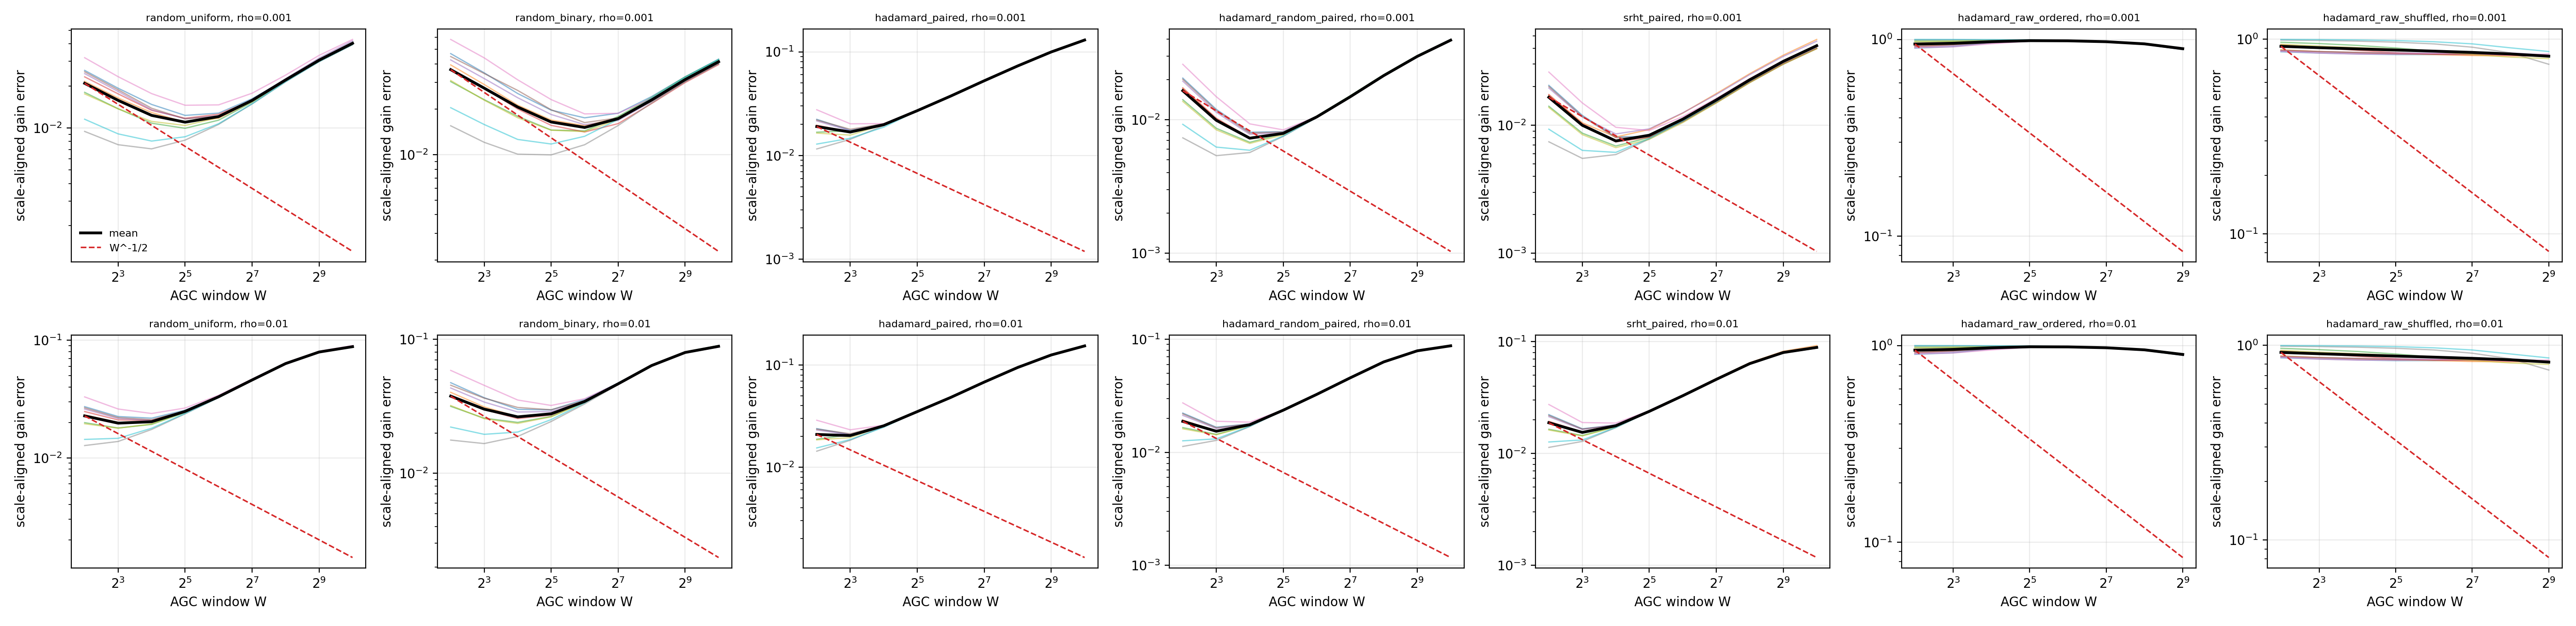
\includegraphics[width=\linewidth]{fig3a_error_vs_W.png}\\
{\footnotesize (a)}
\end{minipage}\hfill
\begin{minipage}[t]{0.30\textwidth}\centering
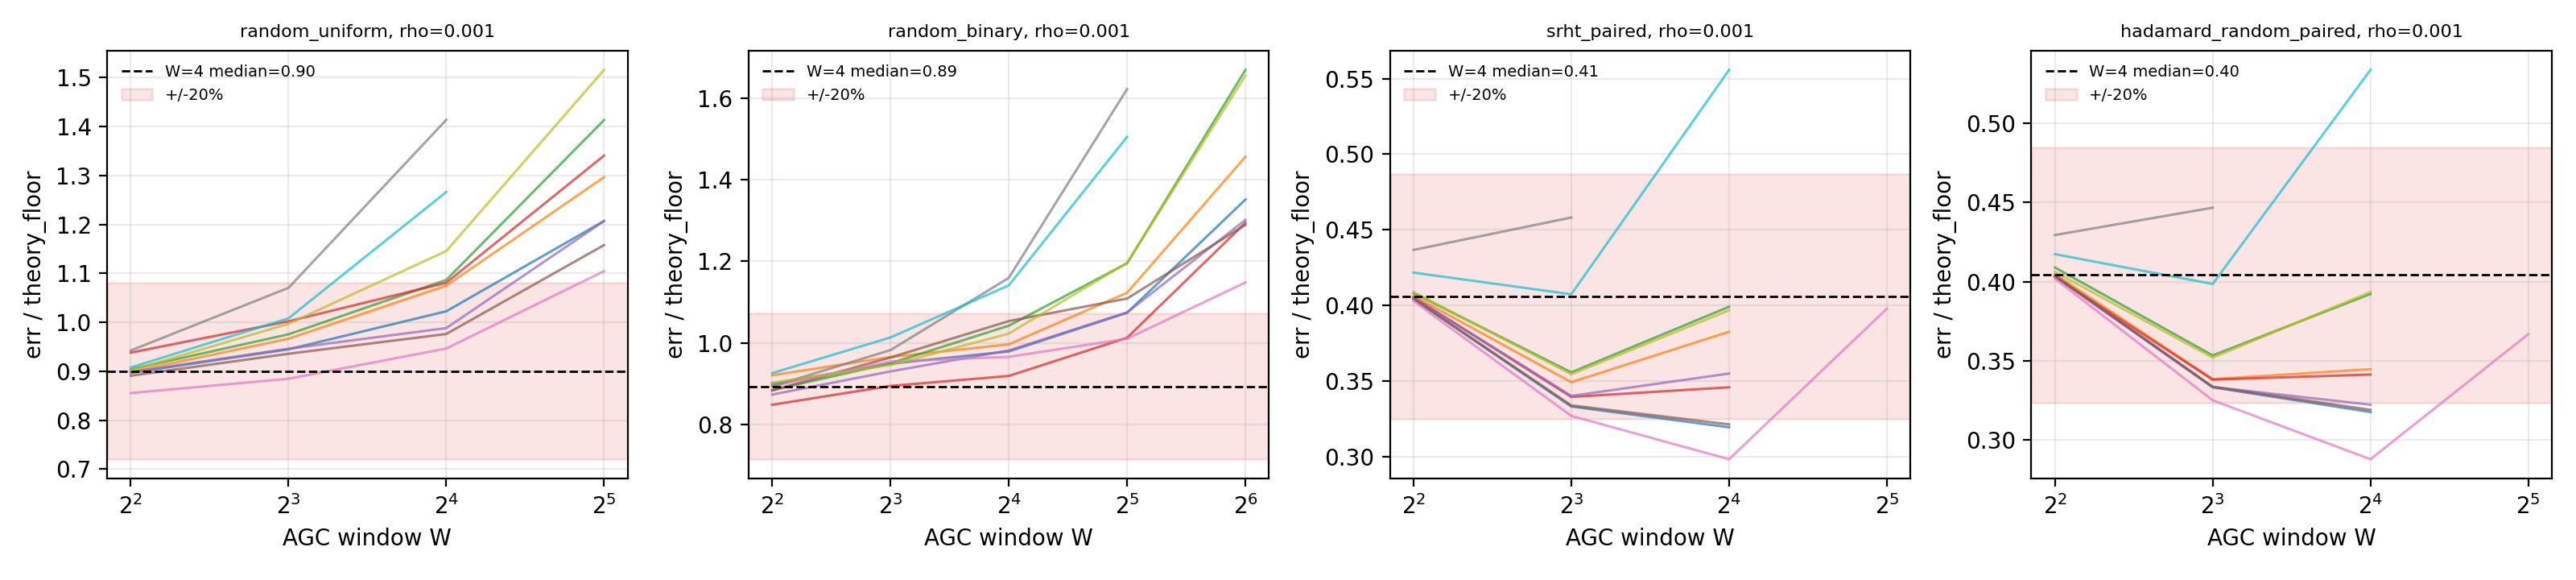
\includegraphics[width=\linewidth]{fig3c_collapse.png}\\
{\footnotesize (b)}
\end{minipage}
\caption{Blind gain identifiability (seven frame-matched arms, 2048 frames each; $32\times32$ objects, $K=1024$; medians over 20 seeds $\times$ 10 objects at $\rho_{\mathrm{pair}}=10^{-3}$, $s=0.1$). (a) Blind gain error $\|\hat a-a\|/\|a\|$ versus window $W$ under the ratio AGC (solid, filled) and the log-window implementation (dashed, open). The latter coincides with the Theorem-B estimator only on originally positive, all-one-mask arms; raw signed-Walsh arms are masked diagnostics. Error bars: two-way clustered 95\% CIs of the median best-window error. (b) Errors normalized by the theory floor $\sqrt{\mathrm{CV}_B^2/W}$ collapse across the ten objects. Quantitative values: Sec.~9.2 and Table~III.}
\end{figure*}

\section{Estimation rate, lower bounds, and low-photon robustness}

Section~5 establishes relative-gain consistency under explicit carrier-window conditions. The baseline is the plain windowed log of Theorem~B. For photon counts we instead average $\psi_\alpha(c)=\log(c+\alpha)$ and invert the per-window calibration curve $M_n(\theta)=\sum_kw_{nk}m_\alpha(\Lambda_0e^\theta b_k+d)$ built from \emph{known} carriers $b_k$: an oracle-known-carrier estimator, distinct from the blind high-count estimator. The homogeneous shortcut $m_\alpha^{-1}(\mathrm{mean}_W\psi_\alpha)$ is exact only for a constant carrier. For fixed $\alpha$, the high-count limit has sensitivity tending to one and approaches the ordinary log behavior; no unqualified joint $\alpha\to0$ limit is used. The window trades smoothing bias against count variance.

\begin{namedthm}{Theorem C (oracle-known-carrier finite-window rate)}
Assume conditionally independent Poisson counts across distinct frames, known positive carriers, a nonempty calibration-safe log-gain interval, and $\beta\in(0,1]$. For the endpoint-clamped calibrated inverse,
\[
\mathbb E[(\hat\theta_n-\ell_n)^2\mid\ell,b]
\le(B_n^2+V_n)/\underline\kappa_n^2,
\]
where $B_n$ is the carrier-weighted smoothing bias, $V_n$ the exact conditional soft-log variance, and $\underline\kappa_n$ the window sensitivity. The optimized power law is asserted only when its unconstrained width is feasible and the sensitivity ratios are uniformly controlled. For arbitrary carriers no $\beta>1$ claim is made; sensitivity-balanced interior windows give the partial extension in Appendix~D.4. (Proof: Appendix~D.)
\end{namedthm}

At $d=0$, direct Poisson Le~Cam/Assouad bounds give the matching local order for a centered log-domain loss chosen to match the blind quotient metric, in the locally-flat-gain, feasible-window regime. The oracle experiment itself fixes the absolute scale through known $\Lambda_0$ and carriers. This Poisson statement is proved directly; it is not inherited from the Gaussian theorem below.

\begin{namedthm}{Theorem D (fixed-Gaussian interior minimax rate)}
In the fixed experiment $Y_n=m+f(n/N)+\varepsilon_n$, $\varepsilon_n\stackrel{\mathrm{iid}}{\sim}\mathcal N(0,\sigma^2)$, impose the gauge $N^{-1}\sum_nf(n/N)=0$, the bounded H\"older class $\mathcal H_\beta^0(L,A)$, and pointwise squared loss at an interior grid point. If $h_*=(\sigma^2/(NL^2))^{1/(2\beta+1)}$ is a feasible centered bandwidth and $Lh_*^\beta\le A/4$, then
\[
\inf_{\hat f}\sup_{f\in\mathcal H_\beta^0(L,A)}
\mathbb E(\hat f-f)^2\asymp_\beta
L^{2/(2\beta+1)}(\sigma^2/N)^{2\beta/(2\beta+1)}.
\]
No three-segment finite-$N$ minimax equivalence is claimed outside this interior regime. (Proof: Appendix~D.)
\end{namedthm}

The floor beneath the blind bound is Fisher geometry: in the gauge quotient (global scale unobservable, Sec.~5) the relevant object is the \emph{quotient Fisher information}, which is singular along the exact ambiguity directions generated by Theorem~A. Non-identifiability is not poor conditioning; it is a genuine flat direction of the likelihood --- the exact collision curve $\ell_u=\ell+u$, $T_u=M^{-1}\operatorname{diag}(e^{-u})MT$ made infinitesimal (tall designs need the range condition of Appendix~D.3; constant $u$ is the gauge).

Which design constant controls what is a spikiness question, and three distinct functionals appear: $K_{\mathrm{eff}}$ governs random-carrier excitation (Prop.~1) and also enters the pairwise-Hadamard residual-gain budget (Prop.~3); $K_\infty$ is the Lindeberg parameter gating the Gaussian approximation and windowed-energy concentration, while the log expansion additionally needs the Appendix~C positivity and tail conditions; $K_4$ enters the permutation-whitening concentration guarantee (Sec.~7, via $\min(\epsilon^2 K_4,\epsilon K_\infty)\ge C\log(K/\delta)$). Conflating them mislabels the bottleneck: a design flat in $K_{\mathrm{eff}}$ can still be spiky in $K_\infty$.

Low photon counts do not break the log domain: the Poisson derivative identity $\frac{d}{d\lambda}\mathbb{E}f(C)=\mathbb{E}[f(C{+}1){-}f(C)]$ gives sensitivity $\kappa_\alpha(\lambda)\to 1$ at high $\bar\lambda$ and $\kappa_\alpha(\lambda)\to\lambda\log(1+1/\alpha)$ as $\bar\lambda\to 0$, and the offset $\alpha$ absorbs empty bins so no frame contributes $\log 0$. Through Theorem~C the photon-starved variance factor obeys the general window law of Appendix~D.4 (actual intensities in the numerator, anchor intensities in the sensitivity denominator), simplifying to $\sim1/(W\bar\lambda)$ only under \emph{local gain flatness} --- where it matches the direct Poisson lower bound at rate level, since at $d=0$ the Poisson Fisher information for a known-carrier log-intensity shift equals the expected intensity $\lambda$ and therefore vanishes as $\lambda\to0$; low expected counts cut precision but never make the estimator diverge (Fig.~5). The reference curve plotted there, $\mathrm{mean}_n[1/I_n]$, is an \emph{oracle common-shift diagnostic}, not a nuisance-path quotient Cram\'er--Rao bound.

The caveat, stated honestly: without calibration inversion, a plain windowed average of $\psi_\alpha$ --- the \emph{uncalibrated proxy} --- becomes shrinkage-bias-dominated at $\bar\lambda\lesssim1$: it is pulled toward $\log\alpha$, and its MSE sits \emph{below} the oracle common-shift diagnostic because bias is present (MSE below $1/I_A$ is compatible with shrinkage bias; MSE above it does not certify unbiasedness --- Appendix~D.4). The calibrated estimator of Theorem~C removes this shrinkage and tracks the $1/(W\bar\lambda)$ law without falling below the diagnostic on the tested grid, giving up precisely the bias-bought low-count MSE discount of the proxy (and of the Anscombe transform \cite{Anscombe1948}) --- quantified in Sec.~9 (Fig.~5).

\section{Basis design: randomized orthogonal acquisition (SRHT)}

Must one surrender orthogonal conditioning to buy the anchor's random illumination? No. The randomized Hadamard transform --- an orthogonal Hadamard carrier composed with a random sign flip and a random pixel permutation, the SRHT of the sketching literature --- keeps a full-rank, well-conditioned forward map while randomizing the \emph{temporal handwriting} of the object: one shuffles the deck without bending the cards. We use the \emph{full} $N=K$ randomized transform throughout; ``subsampled'' is reserved for the $N<K$ case, which raises a bias/prior question outside our scope.

The mechanism is exact. Writing the per-coefficient excitation as $Z_g$ under a random diagonal sign $D$, the residual gain--object coupling is governed entirely by the Walsh spectrum of the squared object. With $w = T^2$,
\[\operatorname{Cov}_D(Z_g, Z_h) = \hat{w}(g+h),\]
the Walsh transform of $w$ at the dyadic index sum. Sign randomization alone gives \emph{exact} pairwise whitening iff $\hat w(k)=0$ for every $k\ne0$; it gives $\varepsilon$-whitening iff $\max_{k\ne0}|\hat w(k)|\le\varepsilon S_2$. These are conditions on the object, not the design: a structured $T$ can concentrate $\hat w$ off the origin, and sign flips cannot remove it.

The random permutation supplies the missing genericity, acting as a probabilistic Walsh-flattener: permuting pixels spreads the mass of $\hat{w}$ across the spectrum, driving the off-origin covariance below tolerance $\varepsilon$ with probability $1-\delta$ once the object is spectrally spread enough,
\[\min\!\big(\varepsilon^2 K_4,\ \varepsilon K_\infty\big) \ \geq\ C \log(K/\delta),\]
with $K_4$, $K_\infty$ the Sec.~6 spread functionals --- both diverge as the object's energy delocalizes and collapse when a few pixels dominate; the bound quantifies how much delocalization the permutation needs.

Permutation is a genuine second ingredient. Under permutation alone,
\[\operatorname{Var}_P Z_g = \frac{K S_2 - S_1^2}{K-1} = S_2\,\frac{K - K_{\mathrm{eff}}}{K-1},\]
so, for the physical nonnegative-object regime $K_{\mathrm{eff}}\ge1$, the residual carries an $O(1/K_{\mathrm{eff}})$ \emph{upper} bound on variance but no matching lower bound: a flat object produces zero excitation, so permutation cannot guarantee two-sided control coefficient by coefficient, and the whitening claim is one-sided unless the sign flip and the spectral-spread condition are both in force. A row-order shuffle of the acquisition sequence is a third, weaker operation: it makes the temporal carrier finite-population exchangeable and, under the Serfling range/variance scaling of Appendix~C, concentrates its random-permutation window means; it does not guarantee ($\star$) for every realized order or two-sided per-coefficient excitation. The ablation of Supplementary Material S1 (Fig.~8) probes the acquisition-time operations (none / row-order permutation / sign / both); its permutation arms reorder acquisition time ($P_{\mathrm{row}}$) and do \emph{not} realize the pixel permutation $P_{\mathrm{col}}$ of the whitening analysis above, whose factorized attribution --- including the $P_{\mathrm{col}}$-only and $P_{\mathrm{col}}{+}D$ arms in natural acquisition order --- is reported in Sec.~9.6 and Appendix~E.6.

\begin{nameddef}{Design rule (blind slow gain)}
(i) Do \emph{not} acquire in ordered Hadamard when the nuisance is a blind, slowly drifting gain --- the ordering hands the object a temporal signature (Sec.~4). (ii) Randomize the carrier: apply the SRHT sign flip \emph{and} permutation. (iii) Verify Walsh-flatness of the realized (permuted) $T^2$, or rely on the permutation bound above with $K_4, K_\infty$ estimated from the object class. (iv) Keep a positivity/offset margin so the log or soft-log stage of Sec.~6 stays away from its singularity. (v) Choose the averaging window $W$ from the bias--variance trade of Sec.~6, not from conditioning.
\end{nameddef}

The rule prescribes \emph{both} randomizations because that configuration has a two-sided theorem guarantee under the stated spectral-spread condition; the ablation (Fig.~8) reports the different, empirical fact that either randomization alone already recovered essentially the full advantage in the tested panel. The two statements must not be merged: the theorem guarantees whitening under its hypotheses, the ablation shows that any tested way of breaking the chronology sufficed here; we do not promote the panel result to a universal claim.

The synthesis: orthogonality and randomized temporal homogenization are compatible. SRHT preserves the $B_L=1$ leverage of a full orthogonal inversion while, under Walsh-flatness or the stated permutation concentration event, controlling cross-row covariance over the pixel-randomization ensemble. A separate $P_{\mathrm{row}}$ randomization gives finite-population exchangeability of acquisition order. Neither statement makes a conditioned fixed draw stationary or mixing; the realized window criterion remains a check.

(Proof of the Walsh identity and permutation bound: Appendix~E.)

\section{From identifiability to images: the reconstruction bridge and phase diagram}

Sections~4--7 answer the statistician's question --- \emph{is the gain identifiable, and at what rate?} --- but the practitioner asks: \emph{how many gray levels do I lose?} This section supplies an exact finite-$N$ second-moment bridge under its stated exogeneity hypotheses. Physical Poisson and signed-coefficient implementations enter through separately derived covariance models.

The corrected bucket record is $z_n=(1+\delta_n)b_n+\xi_n$ with $b=AT$, $\delta_n$ the \emph{residual} multiplicative gain after whatever blind correction the pipeline applied, and $\hat T=Lz$ any linear reconstruction.

\begin{namedthm}{Theorem 1 (master finite-noise relMSE identity)}
Assume --- as part of the hypothesis, not as background convention --- that (H1) $\mathbb{E}\,\xi=0$; (H2) the residual gain $\delta$ and the additive noise $\xi$ are uncorrelated, $C_{\delta\xi}:=\operatorname{Cov}(\delta,\xi)=0$; (H3) the gain estimate $\hat a$ is \emph{exogenous} with respect to the reconstructed record --- computed independently of the noise realization $\xi$ (injected or synthetic residuals, an independent calibration record, or a cross-fitted estimate from held-out frames), so that (H1)--(H2) hold conditionally on the record being reconstructed; and (H4) the second moments $m_\delta$, $V_\delta$, $\Sigma_\xi$ are finite. Then, without Gaussian or small-noise approximation,
\begin{align*}
\frac{\mathbb{E}\|\hat T-T\|^2}{S_2}\;=\;&\underbrace{\frac{\|(LA-I)T+L\,\mathrm{diag}(b)\,m_\delta\|^2}{S_2}}_{\text{bias}}\\
&+\;\underbrace{\frac{\operatorname{tr}\!\big(L\,\mathrm{diag}(b)\,V_\delta\,\mathrm{diag}(b)\,L^\top\big)}{S_2}}_{\text{residual gain}}\\
&+\;\underbrace{\frac{\operatorname{tr}\!\big(L\,\Sigma_\xi L^\top\big)}{S_2}}_{\text{additive noise}}.
\end{align*}
If the residual gains are independent with $\mathrm{Var}\,\delta_n=v$, the gain term collapses to $v\,B_L$ with the \textbf{leverage} $B_L=(1/S_2)\sum_n b_n^2\|Le_n\|^2$; coherent (smooth) residuals require the full matrix form. (Proof: Appendix~F.)
\end{namedthm}

The hypotheses are not decorative: a gain estimate computed from the \emph{same} noisy record carrying $\xi$ --- the generic blind situation --- generically violates (H1)--(H3), adding an $L\,m_\xi$ bias term and a $C_{\delta\xi}$ cross-term (Remark~F.1.1). The identity is accordingly validated in the injected-residual (exogenous) regime (E4, Sec.~9) and applies to cross-fitted estimates restoring (H1)--(H2) by construction; for same-record blind pipelines it is exact only up to those two terms.

For physical nonnegative measurement rows, the Poisson plug-in $\Sigma_\xi=\mathrm{diag}(\tau_{G,n}^2+b_n^2/\Phi_n)$ is exact at all counts after the post-calibration substitution $\hat a_n\to a_n$; before it both variances carry $(a_n/\hat a_n)^2$. A signed transform coefficient $b_n=(UT)_n$ is not a Poisson intensity: complementary masks or a positive offset require their own photon allocation and differencing covariance. The identity uses raw error $\mathbb E\|\hat T-T\|^2/S_2$. Fig.~9 is therefore regenerated with raw total MSE for every theorem-validation arm; scale-aligned MSE remains a separately labeled image-quality output. Specializing $L$:

\begin{itemize}[leftmargin=*,itemsep=1pt,topsep=2pt]
\item \textbf{Orthogonal / SRHT full inversion:} $B_L=1$, so independent residual gain passes through at unit leverage. For signed-coefficient additive covariance $\Sigma_c$, $\mathrm{relMSE}=v+\operatorname{tr}(\Sigma_c)/S_2$; no direct signed-Poisson term is inserted.
\item \textbf{Pairwise (differenced) Hadamard:} gain term $R_{\mathrm{pair}} = (K_{\mathrm{eff}}/4)\,D_H(T)\,\mathbb{E}[\Delta^2]$ --- the second moment $\mathbb{E}\Delta^2$, not $\mathrm{Var}(\Delta)$, unless $\mathbb{E}\Delta=0$ is separately assumed (a deterministic mismatch $\Delta\equiv\epsilon$ has zero variance but nonzero risk; Appendix~F.3.2) --- with $D_H\approx 1$ for non-DC coefficients and $\mathbb{E}[\Delta^2]\approx 2s^2\,r(\rho_{\mathrm{pair}})$ the adjacent-pair increment for OU drift ($r(\rho)=1-e^{-\rho}$; $r(\rho)\approx\rho$ for small $\rho$): differencing converts \emph{slowness} directly into suppression.
\item \textbf{Random / DGI:} $\mathrm{relMSE}_{\mathrm{DGI}} = C_0^{\mathrm{floor}}/N + (1+C_0^{\mathrm{lev}})v/N + $ noise terms. Three constants of the \emph{same} pipeline must be kept apart (Appendix~F.3.3): the fixed-design sampling floor $C_0^{\mathrm{floor}}$ (raw $\approx10^3$ here, aligned $\approx7\times10^2$ --- a factor-1.54 metric difference), the drift leverage $\Lambda_{\mathrm{lev}}=NB_L=1+C_0^{\mathrm{lev}}$, and the population moment constant $K+\beta_4-2$. Mean subtraction removes the $K_{\mathrm{eff}}K(\mu/\sigma)^2$ background penalty from the floor but \textbf{not} from the leverage --- drift modulates the large DC background coherently --- so for mean-subtracted pipelines $C_0^{\mathrm{lev}}$ is the nonnegative-background value of (F.10), roughly $10^3\times$ the floor. There is \textbf{no universal $C_0$}: each constant depends on pattern statistics, background, normalization, \emph{and metric} --- for our SCGI-style testbed \cite{PengChen2024APL} the measured values are used throughout Fig.~9 and Fig.~4.
\end{itemize}

In the square unit-leverage comparisons studied here, orthogonal inversion is the reference conduit: $B_L=1$ and there is no reconstruction floor. This is not a universal optimum over redundant designs --- repeated or averaged measurements can have $B_L<1$. The randomized arms win here primarily because the stationarity anchor lets the residual error itself shrink, where ordered chronology offers no comparable blind handle.

These closed forms compete, producing a finite-$N$ flip boundary.

\begin{namedthm}{Prop 3 (finite-$N$ flip boundary; fixed-point form)}
All risks are the \emph{raw} relative MSEs of Theorem~1. Write the random-arm risk as $R_{\mathrm{rand}}=C_0^{\mathrm{floor}}/N+\Gamma_{\mathrm{blind}}+R_{\mathrm{rand,noise}}$, where $\Gamma_{\mathrm{blind}}$ is the full residual-gain contribution. For an exogenous, centered, frame-uncorrelated residual only, $\Gamma_{\mathrm{blind}}=(1+C_0^{\mathrm{lev}})q_{\mathrm{blind}}/N$. A same-record blind estimator requires the full projected mean, covariance, and residual--noise cross terms and has no asserted scalar $v_{\mathrm{blind}}$ representation. In the scalar special case, $\rho^{*}=\inf\{\rho_{\mathrm{pair}}\ge0: R_{\mathrm{pair}}\ge R_{\mathrm{rand}}\}$ satisfies
\[
\begin{aligned}
1-e^{-\rho^{*}}=\frac{2}{K_{\mathrm{eff}}\,D_H\,s^{2}}\big[&C_0^{\mathrm{floor}}/N\\
&+\Gamma_{\mathrm{blind}}(\rho^*,N)\\
&+R_{\mathrm{DGI,noise}}-R_{\mathrm{pair,noise}}\big],
\end{aligned}
\]
Because the right side moves with $\rho^*$, this is not an explicit solution: existence needs a crossing and uniqueness a single-crossing condition. Only a constant bracket $Q_0$ gives $\rho^*=-\log(1-Q_0)$; $Q_0\ge1$ gives no finite crossing. Its gain-known leading heuristic is $\rho^{*}\approx2C_0^{\mathrm{floor}}/(NK_{\mathrm{eff}}s^2)$. (Proof: Appendix~F.)
\end{namedthm}

\emph{Remark:} $\rho_{\mathrm{pair}}$ (adjacent-pair decorrelation, this section) and $\rho_{\mathrm{bw}}$ (normalized bandwidth, Sec.~4) both grow with drift speed but are not equal; every Fig.~4 axis declares its convention (Appendix~F.4).

The injected-residual bridge is tested in raw MSE in Supplementary Material S2 (Fig.~9); because the protocol contains no photon noise, it isolates residual-gain propagation. Figure~4 reports the equal-frame competition and the no-free-parameter gain-known skeleton. The same-record blind no-flip result is an empirical observation accompanied by a conditional noiseless projected-covariance diagnostic, not a scalar theorem validation. Three operational regimes still organize the chart: slow drift favors pair differencing, intermediate drift favors randomized chronology, and fast drift defeats blind separation unless an external gain reference is supplied.

The measured constants and conventions behind Fig.~4 are collected in Table~I.

\begin{table*}[!t]
\centering
\caption{Headline measured constants behind Fig.~4 (secondary constants and grid conventions: Supplementary Material Table~II). Every constant is pipeline-specific, and floor, leverage, and moment constants of the \emph{same} pipeline are different numbers (Appendix~F.3.3). Confidence intervals: two-way (seeds-and-objects) crossed cluster bootstrap percentile intervals over the 20-seed $\times$ 10-object replication, slope fits restricted to $W\le16$; an object$\times$seed bootstrap treating the 200 cells as independent understates uncertainty; no qualitative conclusion changes.}
\label{tab:constants}
\begin{tabular}{@{}p{0.24\textwidth}p{0.50\textwidth}p{0.20\textwidth}@{}}
\toprule
Quantity & Value in this pipeline & Uncertainty \\
\midrule
Drift leverage $\Lambda_{\mathrm{lev}}=NB_L=1+C_0^{\mathrm{lev}}$, distinct from the Prop.~3 raw floor & $\Lambda_{\mathrm{lev}} \in (7.527\text{--}7.544)\times10^{5}$ across $N$ & exact fixed-operator column-norm calculation, then mean over 10 objects; no residual probe \\
\addlinespace
$D_H(T)$ (pairwise-Hadamard factor) & measured over the ten-object panel: min/median/max $=0.971/0.988/0.999$ (per object via the analytic identity $D_H(T)=\frac{1}{K}\sum_k(1-x_k^2)^2$, $x_k=c_k/S_1$) & deterministic per object (identity evaluated on the panel); no resampling needed \\
\addlinespace
Same-record blind residual & report raw $q_\delta$, residual mean, lag correlation, and projected covariance; scale-aligned gain error is secondary & conditional noiseless proxy, not a scalar theorem input \\
\addlinespace
Prop.~3 boundary, raw metric on both sides & true-$S_1$: $40/40$, median/max factors $\mathbf{1.020}/1.037$, slope $-2.12044$; production median normalization: $40/40$, $1.044/1.200$, slope $-2.00656$; prediction $-2.11371$ & same-estimator validation versus production robustness, identical OU traces; clean-commit authoritative R15 result \\
\bottomrule
\end{tabular}
\end{table*}

\begin{figure*}[!t]
\centering
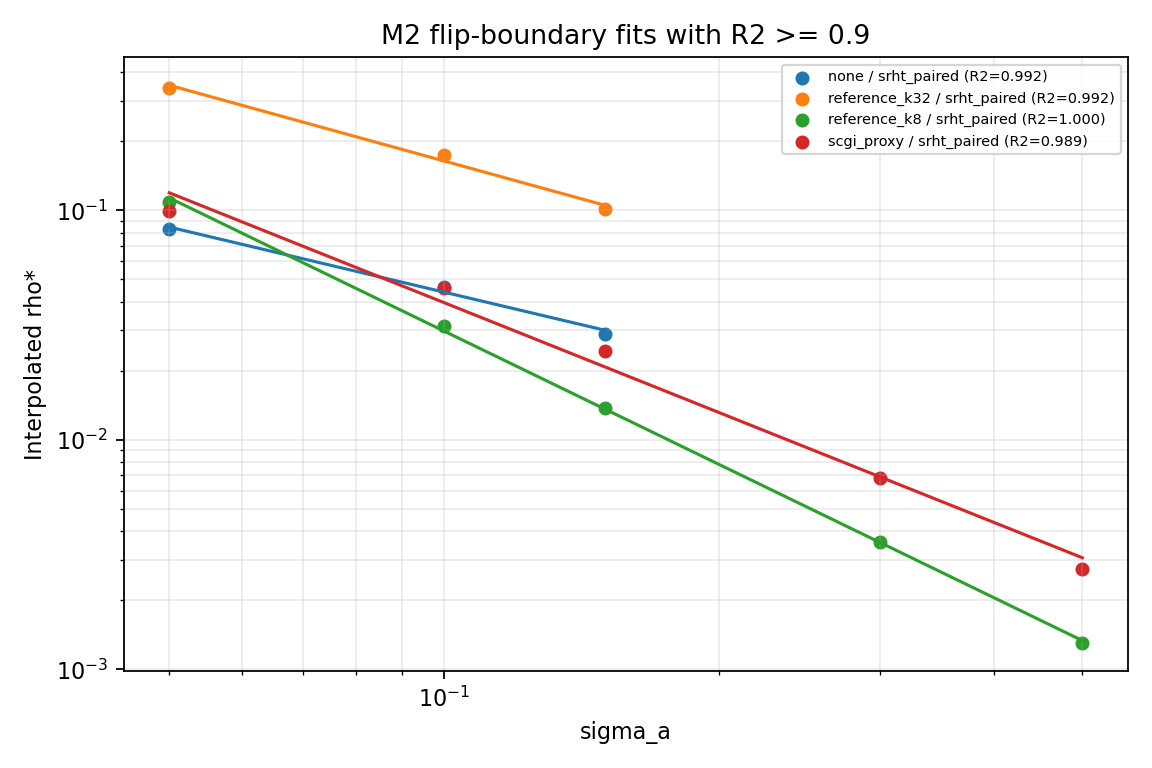
\includegraphics[width=0.56\textwidth]{fig5_flip_boundary.png}
\caption{Empirical winner map, SRHT crossover, and the raw-MSE Prop.~3 skeleton test at equal frame budget ($N=2048$, $K=1024$, OU drift). (a) Winner per $(\rho_{\mathrm{pair}},\sigma_a)$ cell among candidates passing the above-floor gate (grey: floor; outline: the single non-SRHT winner). (b) Descriptive SRHT-paired-versus-ordered-Hadamard crossover fits, a comparison Prop.~3 does not rank. (c) No-free-parameter gain-known skeleton: prediction and factor-2 band against the theorem-faithful true-$S_1$ arm (filled circles) and production median normalization (open squares) on identical traces; triangles: no crossing in range. True-$S_1$ median/max factors are $1.020/1.037$; production factors $1.044/1.200$.}
\end{figure*}

\section{Numerical experiments}

The theory of Secs.~4--8 makes quantitative predictions --- a stationarity dichotomy, a leading Gaussian/log-variance $W^{-1/2}$ law whose tested-panel object dependence is summarized by $K_{\mathrm{eff}}$, an exact relMSE identity, a flip boundary, and a photon-limited Fisher scaling --- and this section tests each. A closing subsection integrates five later verification experiments: the tall-design rank threshold (Fig.~6), whitening power (Supplementary Material S1), the coherent-residual validation of Theorem~1 (S2), the $C_0$ audit, and oracle-to-blind baselines (S3).

\noindent\textbf{Protocol.} All results are simulations; no hardware data enter. Comparisons use matched frames and flux. Each seed shares one OU log-gain trace across arms. The H\"older model is the analysis class, whereas OU is the simulation protocol and is not pathwise Lipschitz. Ten fixed objects span $K_{\mathrm{eff}}=59.8$--$864.3$; the base seed is $20240708$. Blind gain error is scale-aligned after unit-mean normalization; mask contrast is GT-mask CNR. Theorem~1 and Prop.~3 validation use raw reconstruction MSE, while scale-aligned reconstruction MSE is retained only as a separately labeled image-quality metric. Full enumerables: Supplementary Material S5.

\noindent\textbf{Carrier stationarity (Fig.~2).} This experiment applies a \emph{variance-stationarity diagnostic} to the noiseless carrier $\{B_n\}$ before any gain is applied (8192 frames per arm, $64\times64$ objects). The Brown--Forsythe test checks chunk-variance equality: it screens the stronger strict-stationarity sufficient model used in (B2), not the windowed log-mean condition ($\star$) itself and not a necessary condition for ($\star$). The test at $p<10^{-3}$ rejects 7 of 10 objects for ordered Hadamard, with $p$ reaching $10^{-20}$, against 0 of 10 for both i.i.d.\ random ensembles (uncorrected per-test $p$-values; the strongest rejections clear a Bonferroni-adjusted threshold by many orders of magnitude). The permuted arms --- randomly permuted paired Hadamard ($P_{\mathrm{row}}$) and SRHT ($P_{\mathrm{row}}{+}D$, Appendix~E.6) --- each reject 2 of 10: a \emph{fixed} reordering draw does not guarantee temporal homogeneity for every object, since the randomization guarantees of Secs.~5 and 7 are probabilistic over draws --- this residue is the theory's own prediction, not an anomaly. The pixel-level randomization of the SRHT analysis ($P_{\mathrm{col}}$, $D$) is probed by the factorized ablation of Sec.~9.6. The Parseval invariant closes the loop: every exhaustively paired arm has carrier $\mathrm{CV}_B = 1/\sqrt{K_{\mathrm{eff}}}$ to about $10^{-6}$ relative accuracy, and the random arms match $(\sigma_I/\mu_I)/\sqrt{K_{\mathrm{eff}}}$ within $\pm2\%$ --- the ordered pathology lives entirely in the temporal variance structure, not in the marginal spread (descriptive counts over the ten-object panel).

\noindent\textbf{Blind gain identifiability (Fig.~3).} This is the core evidence for Theorem~B, run over nine arms including the raw, non-paired Hadamard arms that feed bare signed Walsh coefficients to the estimator (bucket convention (i), diagnostic-only); per-arm errors and slopes with two-way CIs: Supplementary Material Table~III. Raw arms are scored at the same 2048-frame budget; the single-pass 1024-frame diagnostics are indistinguishable (Table~III), so the failure is chronology, not budget. In Fig.~3 the chronology failure of Theorem~A is made visible: under the ratio AGC the raw ordered arm's blind gain error is $0.94$--$0.99$ across all averaging windows (median best-window $0.899$) and does not decay; shuffling the raw frames improves this to $0.794$ --- permutation helps even here --- but the arm remains far above the random and paired arms at $0.007$--$0.017$, because without pairing the near-zero-mean carrier leaves the AGC ill-posed. The log-window implementation coincides with the Theorem~B estimator only on arms whose original analyzed carrier is strictly positive (so the positivity mask is all one); on raw signed arms it is an endogenous masked diagnostic, not a theorem test. It agrees with the ratio AGC to about $2\%$ on all positive stationary-carrier arms with the same qualitative ordering; on the raw diagnostics, ordered still cannot fall below $0.71$ (non-decaying) while shuffled improves to $0.136$, still at least $12\times$ above every randomized arm. Within the variance-obeying arms, the slow-drift variance-segment slopes of $\log(\mathrm{err})$ against $\log W$ all sit inside the $W^{-1/2}$ band ($-0.39$ to $-0.61$), while naturally ordered paired Hadamard is shallow at $-0.24$: differencing cancels the drift within pairs but leaves the ordered envelope. Normalizing by the theory floor $\sqrt{\mathrm{CV}_B^2/W}$ collapses the panel: the paired arms sit at $0.40$--$0.41$ and the random arms at $0.89$--$0.90$, each bundle within $\pm5$--$7\%$ across all ten objects, and the best-window error correlates with $K_{\mathrm{eff}}$ at $-0.86$ to $-0.90$ (descriptive) --- consistent, within this tested panel, with the object entering through $K_{\mathrm{eff}}$ alone, as Proposition~1 predicts to leading Gaussian/log-variance order. The shuffled-paired arm performing like the random arms bears out the permutation analysis of Sec.~7: pairing cancels the slow drift within pairs, and the permutation restores the stationarity that the ordering destroyed.

The 20-seed uncertainty replication (31{,}600 rows) confirms these slopes under the fixed $W\le16$ variance-segment convention: the randomized arms' median two-way slopes lie between $-0.39$ and $-0.62$, the naturally ordered paired arm's ratio-AGC slope CI straddles zero (no detectable decay), and the raw ordered arm stays essentially flat at $0.899$ (per-arm values and CIs: Table~III). The two-way crossed cluster bootstrap widens naive object$\times$seed intervals by $3$--$5\times$ without crossing any qualitative boundary (rationale: Table~I caption). One nuance: under the log-domain estimator the naturally ordered paired arm shows a shallow decay ($-0.222$ $[-0.306,-0.054]$) where the ratio AGC shows none; both remain far outside the $W^{-1/2}$ band, so the chronology conclusion stands (``no detectable decay'' attaches to the ratio AGC). Best-window blind gain errors at this operating point are in Table~I; the exploratory slopes and $R^2$ above used an adaptive variance segment, and the two conventions agree on every qualitative conclusion.

\noindent\textbf{The reconstruction bridge (Supplementary Material S2, Fig.~9).} The R15 bridge uses one metric and one quantity in every arm: total \emph{raw} relative MSE versus the fixed-design prediction $R_{\mathrm{floor}}^{\mathrm{raw}}+B_Lv$. The balanced 8100-row protocol contains three reconstructors, $N\in\{1024,2048,4096\}$, six $v$ levels (including the $v=0$ baseline), ten objects, and fifteen seeds. The deterministic inverses remain flat in $N$ (per-$v$ slopes $[-0.117,0.112]$ orthogonal and $[-0.014,0.009]$ SRHT), while random/DGI follows $1/N$ (slopes $[-1.005,-0.972]$). Across the $(N,v)$ aggregates, measured/theory ratios lie in $[0.913,1.163]$ for the orthogonal inverse, $[0.992,1.021]$ for SRHT, and $[0.982,1.010]$ for random/DGI; exact fixed-operator leverage gives $NB_L=(7.527\text{--}7.544)\times10^5$. The former DC-object discrepancies were created by scale alignment and disappear from the raw theorem panel. The per-realization identity $R_{\mathrm{raw}}=R_{\mathrm{floor}}+R_{\mathrm{gain}}+R_{\mathrm{cross}}$ closes to $2.28\times10^{-7}$ absolute error. The clean-commit r3 output is the submission-authoritative bridge dataset.

\noindent\textbf{Phase diagram and ablation (Fig.~4; ablation panels in Supplementary Material S1, Fig.~8).} The phase diagram sweeps $\rho\in[10^{-3},10]$ and $\sigma\in[0.05,0.5]$ at equal frames. Of 29 above-floor cells, SRHT-paired acquisition wins 28; one goes to randomly ordered pairwise Hadamard with SCGI-proxy correction. The plotted two-parameter crossover fits summarize SRHT-paired versus ordered Hadamard and are not a Prop.~3 test. The no-free-parameter raw-MSE test is separate and now has two explicit estimators on identical OU traces. The theorem-faithful true-$S_1$ arm observes 40/40 crossings at $\sigma_a\ge0.1$, with median/max agreement factors $1.020/1.037$ and pooled slope $-2.12044$ versus the predicted $-2.11371$. The production median-normalized arm also observes 40/40, with factors $1.044/1.200$ and slope $-2.00656$; it is governed by (F.7a) and is a robustness check, not the same-estimator validation. The previous factor $1.54$ was a raw/aligned mismatch. The blind random arm never overtakes ordered pairwise Hadamard in the 100 scanned cells. Because its estimator uses the same noiseless record, the R15 analysis reports raw $q_\delta$ and the exact projected mean/covariance decomposition and retains the scalar no-flip curve only as a conditional proxy; no detector-noise cross term is tested. The intermediate-drift winner is SRHT-paired acquisition. The ablation at $\rho=10^{-3}$ gives $+5.45$ dB for SRHT, $+5.47$ dB for pixel signs alone, and $+5.39$ dB for acquisition-order permutation alone (descriptive, nonadditive). At $\rho\ge1$ all blind variants approach the noise floor within $\pm0.09$ dB; this is not a direct low-pass-threshold test unless $\rho_{\mathrm{bw}}$ and $\rho_{\mathrm{pair}}$ are controlled separately.

\noindent\textbf{Low-photon robustness (Fig.~5).} This experiment tests the soft-log analysis of Sec.~6 under Poisson counting, with \emph{five} estimator arms on the same paired Poisson draw at each budget: naive clipped log, Anscombe, the uncalibrated soft-log proxy, the mean-Poisson calibrated proxy $m_\alpha^{-1}(\mathrm{mean}_W\,\psi_\alpha)$, and the oracle-known-carrier calibrated soft-log of Theorem~C (per-window carrier-calibration root, carriers $b_k$ from the simulation truth --- a flat-field benchmark; requested $W=64$, effective interior width 65; truncated edge windows; Appendix~D.4); each point aggregates 50 object-by-seed cells, error bars the SD over those cells. Every ratio below is a log-domain (centered-log-gain) mean-MSE ratio, numerator over denominator as named --- the metric comparable to the oracle common-shift diagnostic $\mathrm{mean}_n[1/I_n]$ of Appendix~D.4 ($d=0$). At mean counts $\bar\lambda\le1$ the naive clipped log is $24.9$--$28.7\times$ worse than the uncalibrated proxy, $16.3$--$21.0\times$ worse than Anscombe, and $1.8$--$11.4\times$ worse than the calibrated estimator (all naive-over-method ratios). The two calibrated arms track the $1/(W\bar\lambda)$ law across the variance regime --- slopes $-1.000$ (oracle-carrier) and $-0.99$ (mean-Poisson proxy, overlapping the oracle arm to $0.4\%$ at this protocol's small carrier variation) over $\bar\lambda\in[2,32]$, against $-0.920$/$-0.732$ for the uncalibrated proxy (its $[1,16]$ fit is contaminated by its own bias transition). At budgets $\bar\lambda\le2$ the uncalibrated proxy and Anscombe fall \emph{below} the common-shift diagnostic --- shrinkage bias, not super-efficiency (MSE above it likewise does not certify unbiasedness; Appendix~D.4) --- whereas the calibrated estimator stays above it at every tested budget, within $2$--$18\%$ at $\bar\lambda\le1$ and $14$--$31\%$ through $[2,32]$. The proxy's apparent $1.19$--$1.53\times$ advantage over Anscombe at these budgets is that shrinkage bias, not efficiency; and the calibrated estimator loses to Anscombe in mean MSE at $\bar\lambda\le1$ (Anscombe $1.8$--$8.9\times$ better) --- a bias-bought advantage (Sec.~6 trade-off) --- overtaking it only for $\bar\lambda\ge32$, where the pairwise ratios converge to $1.00$ ($\pm4\%$). At the high-photon end the floor is drift-limited, not photon-limited: $2.434\times10^{-4}$ ($\rho=10^{-3}$) $\to$ $1.411\times10^{-4}$ ($\rho=10^{-4}$) for the proxy arms, $2.168\times10^{-4}\to1.125\times10^{-4}$ for the oracle-carrier estimator --- $10.92\%$ lower at $\rho=10^{-3}$ and $20.28\%$ at $\rho=10^{-4}$ (two distinct margins), since it deconvolves the known carrier (floor probe: Supplementary Material S4, Fig.~12).

\begin{figure}[!t]
\centering
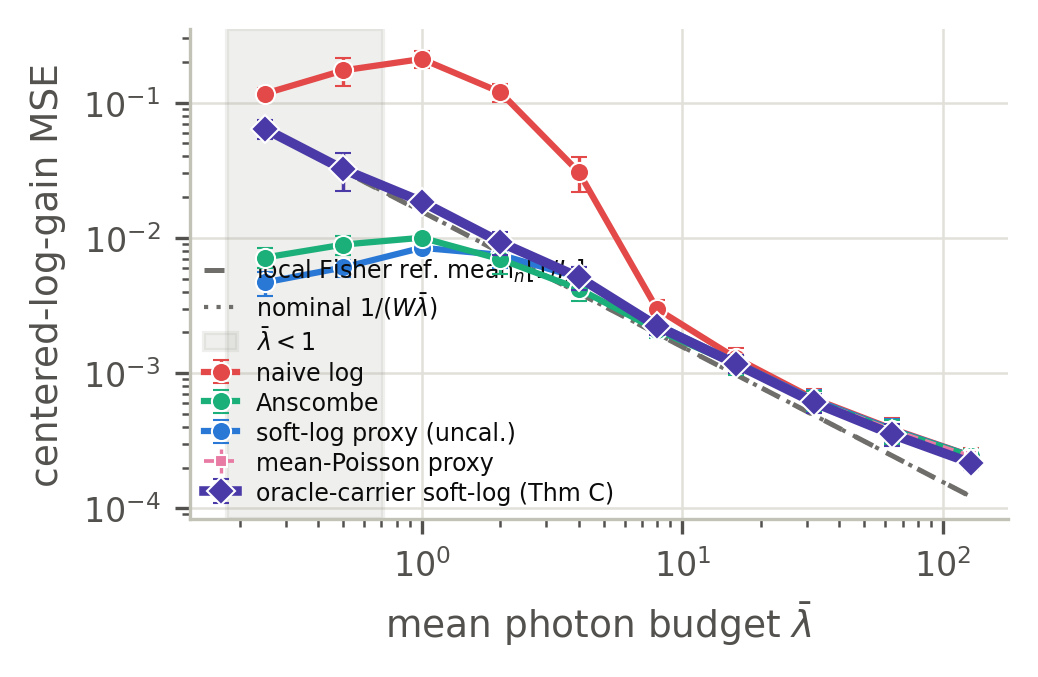
\includegraphics[width=0.46\columnwidth]{fig7_logMSE_vs_photon.png}
\caption{Low-photon robustness under Poisson counting, on identical random-basis carriers and shared gain traces (soft-log $\alpha=0.5$, requested $W=64$ / effective interior width 65, $\rho_{\mathrm{pair}}=10^{-3}$, $s=0.1$; truncated edge windows). Five methods --- naive clipped log, Anscombe, uncalibrated soft-log proxy, mean-Poisson calibrated proxy, oracle-known-carrier calibrated soft-log (Theorem~C) --- on the same paired Poisson draws; error bars: SD over the 50 object-by-seed cells. Centered-log-gain MSE ($d=0$) versus $\bar\lambda$ against the \emph{oracle common-shift diagnostic} $\mathrm{mean}_n[1/I_n]$ (dashed; dotted: nominal $1/(W\bar\lambda)$; shaded: $\bar\lambda<1$) --- not a nuisance-path quotient CRB. The calibrated arms (diamonds: oracle-carrier root; the mean-Poisson proxy overlaps it) track the $1/(W\bar\lambda)$ law and stay above the diagnostic; the uncalibrated proxy and Anscombe buy low-count MSE with shrinkage bias (below the diagnostic at $\bar\lambda\le2$). Ratios, slopes, floor: Sec.~9.5.}
\end{figure}

\noindent\textbf{Threshold, whitening-power, and accountability verifications (Fig.~6 and Supplementary Material S1--S4).} Five further experiments close the remaining theory--evidence gaps; unless a bootstrap interval is stated, every number below is a descriptive result of its grid.

\emph{Tall-design threshold scan (Fig.~6).} A direct test of the local component of Theorem~A$'$ at two object sizes ($K=64$: 20 seeds per cell, 1300 cells; $K=128$: 30 seeds per cell, 1950 cells), over five low-pass drift dimensions $p\in\{3,5,9,17,33\}$ at margins $N-K-p\in[-8,+16]$. At both sizes the local rank test on the collision Jacobian transitions from $0\%$ to $100\%$ pass \emph{exactly} at margin $N-K-p=-1$ for every $p$ (3250 cells, no exceptions) --- matching the proved a.e.\ rank formula $\operatorname{rank}D\Phi_M=\min\{N,K+p-1\}$ of Theorem~A$'$(i); below the wall the observed rank deficits correspond, by the same theorem, to genuine positive-dimensional alias families, not numerical degeneracy. Being a rank statement, the scan verifies the local component only, not the global sufficiency thresholds of A$'$(ii)--(iii) or their conjectured sharpness. The companion solver panel (blind alternating recovery, 8 restarts $\times$ 150 iterations) starts at the same wall but climbs slowly --- about $2\%$ success at margin $0$ and $\sim50\%$ at margin $+16$ for $K=64$ ($\sim41\%$ for $K=128$) --- an \emph{algorithmic-recovery} observation, not a uniqueness test: uniqueness and recovery separate, as Sec.~2's third notion anticipates.

\emph{Multi-permutation whitening power and factorized randomization ablation (Supplementary Material S1, Fig.~7).} Two randomization semantics must be kept separate (Appendix~E.6): the pixel-level randomization of the SRHT theory ($P_{\mathrm{col}}$, $D$; acquisition-order-invariant by Lemma~E.1) and the acquisition-order reordering $P_{\mathrm{row}}$, which is what the Brown--Forsythe screen probes. The factorized ablation attributes the whitening-power headline: either permutation alone substantially reduces the rejection rate --- from $70\%$ (ordered) to $5.6\%$ ($P_{\mathrm{col}}$) and $12.2\%$ ($P_{\mathrm{row}}$), the theory's $P_{\mathrm{col}}{+}D$ to $11.9\%$ in natural order --- a large but incomplete suppression (all three stay well above the $\sim0.1\%$ nominal rate of the $p<10^{-3}$ test), so Appendix~E's whitening claims do not depend on the row-order confound; pixel signs alone barely move it ($43.4\%$). The per-draw Walsh certificate fails (Spearman $0.092$, $p=0.10$): an honest null, consistent with the probabilistic nature of permutation whitening (Sec.~7).

\emph{Coherent-residual validation of Theorem~1 (E4, Supplementary Material S2, Fig.~10).} Under five injected residual-covariance structures (150 cells, raw identity-verification metric), the matrix law of Theorem~1 tracks the measured relMSE within $4.2\%$, while the scalar $v\,B_L$ law --- exact for the orthogonal and SRHT inversions --- fails by up to $3.65\times$ for random/DGI under low-pass-coherent residuals: a direct verification of the coherent clause. E4 uses \emph{injected} residuals; it does not probe the same-record $\delta$--$\xi$ dependence flagged after Theorem~1.

\emph{$C_0$ audit and oracle-to-blind baselines (Supplementary Material S3, Fig.~11).} The measured one-sample constant agrees with the Appendix-F moment formula to $0.35\%$ mean ($2.01\%$ worst) relative error over four ensembles $\times$ five objects, the ensemble spread confirming that $C_0$ is pipeline-specific; and on four held-out objects the ordering static $\ge$ oracle $\ge$ blind-AGC $\ge$ no-correction holds in CNR for 4 of 4, with an oracle$-$blind gap of only $0.035$--$0.147$: the blind estimator concedes little to a gain oracle; forgoing correction costs the most.

\begin{figure}[!t]
\centering
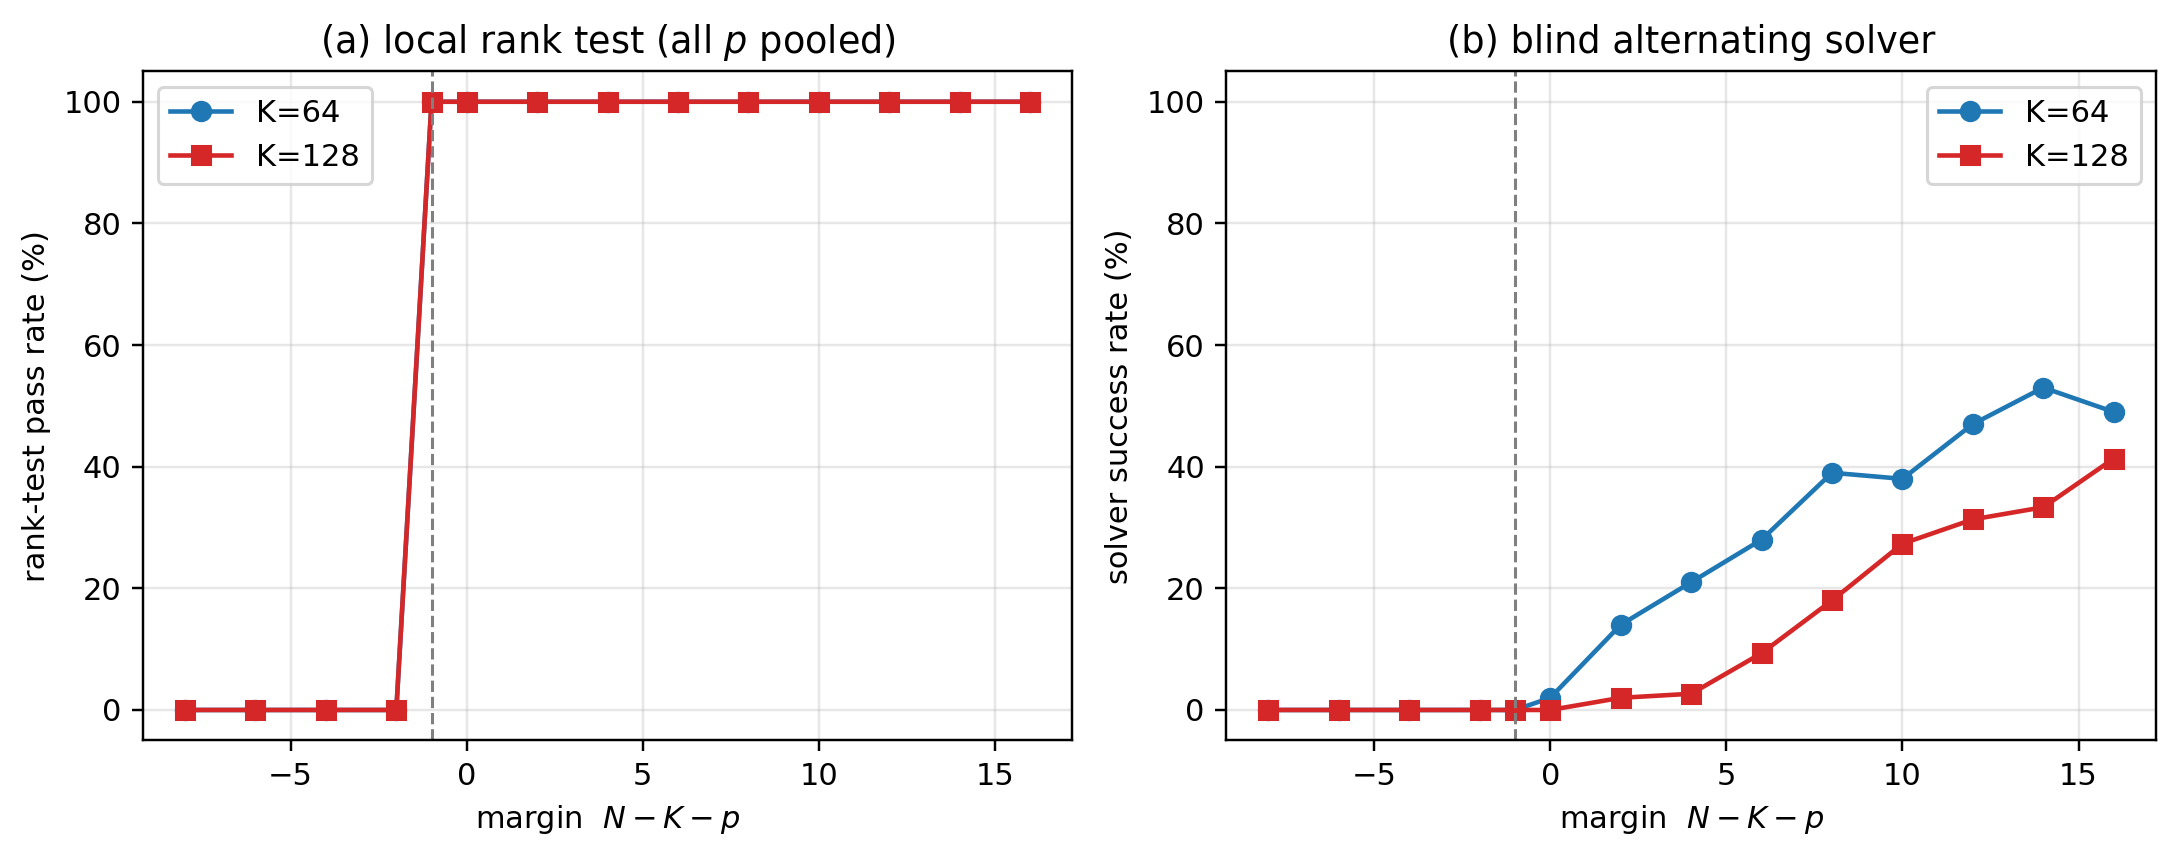
\includegraphics[width=0.55\columnwidth]{fig8_threshold.png}
\caption{Tall-design threshold scan (local-rank test of Theorem~A$'$(i) plus an algorithmic-recovery probe) at $K=64$ (20 seeds/cell, 1300 cells) and $K=128$ (30 seeds/cell, 1950 cells), $p\in\{3,5,9,17,33\}$, margins $N-K-p\in[-8,+16]$, all $p$ pooled. (a) The rank test transitions $0\%\to100\%$ \emph{exactly} at margin $-1$ at both sizes (3250 cells, no exceptions), verifying $N=K+p-1$. (b) The blind alternating solver starts at the same wall but climbs slowly --- algorithmic recovery, not uniqueness; rates in Sec.~9.6.}
\end{figure}

\section{Discussion: significance, scope, and outlook}

The results of Sections~2--9 are pre-acquisition design tools, evaluated on the illumination basis and the expected drift \emph{before} photons are collected. Four deliverables follow, then limits and the invited experimental program.

\noindent\textbf{A go/no-go identifiability predictor.} The tall-design thresholds of Theorem~A$'$ convert ``will this acquisition self-calibrate?'' into arithmetic. For $K\ge2$ and almost every design--object pair with nonvanishing carrier, ordinary local identifiability holds iff $N\ge K+p-1$; generic exact sufficiency begins at $N\ge K+p$, and uniform sufficiency at $N\ge 2K+p-1$, for any fixed drift class $S\ni\mathbf 1$ including the physical low-pass family (sharpness of the two global thresholds remains a labeled prediction). The $K=1$ stratum is globally identifiable on the nonvanishing-carrier set at every admissible $N$. Through $p\approx\rho_{\mathrm{bw}}N$, slow drift needs only modest oversampling, while $\rho_{\mathrm{bw}}\to1$ defeats blind algebraic separation and forces an external reference, an additional prior, or another non-algebraic information source. Theorem~B is one such statistical route only when a coherence window satisfying (B3)--(B4) still exists; it also degrades once gain decorrelates within that window (the $\rho\ge1$ convergence in Fig.~8).

\noindent\textbf{An SRHT design rule.} When blind slow gain is the operative nuisance, do not run ordered Hadamard: its chronology hands the object a temporal signature indistinguishable from drift. Randomize the carrier per the Sec.~7 rule, keeping the two permutation semantics distinct (Appendix~E.6): $P_{\mathrm{col}}$ enters the covariance-whitening guarantee, $P_{\mathrm{row}}$ the exchangeability anchor of Sec.~5; empirically either permutation alone substantially reduces the non-stationarity screen's rejections, signs alone barely (Sec.~9.6). Retain a positivity/offset margin and choose $W$ from the bias--variance tradeoff: statistical self-calibration without surrendering orthogonal conditioning.

\noindent\textbf{A design map exposed to falsification.} Theorem~1 and Prop.~3 organize raw MSE over basis, drift, and noise, with $\rho_{\mathrm{pair}}$ distinct from $\rho_{\mathrm{bw}}$. The true-$S_1$ same-estimator arm validates the gain-known skeleton at median factor $1.020$; the production median normalization gives $1.044$ and needs its additional gauge and cross terms. The earlier factor $1.54$ was a raw/aligned mismatch. For same-record blind DGI, the full projected covariance is the rigorous empirical object; the scalar no-flip curve is only a conditional proxy consistent with the 100/100 observed no-flip cells. Floor and leverage remain pipeline- and metric-specific.

\noindent\textbf{A cross-domain principle.} The exportable statement is basis-agnostic: \emph{to self-calibrate a multiplicative nuisance, design the carrier so its local averages are time-homogeneous and concentrate in the nuisance coordinate.} Blind gain/phase calibration, flat-field correction, coded-aperture and computational microscopy, and single-pixel spectroscopy share this bilinear structure --- analogues and motivation, not proven domains; each needs its own operator analysis of the diagonal-row map \cite{LiLeeBresler1501.06120,KechKrahmer1603.07316}.

\noindent\textbf{Scope and limits.} The claims are theory and simulation only, with no hardware validation. Uniqueness near $N=K+p$ is an identifiability statement, not a conditioning guarantee (stability is a separate random-matrix question), and sharpness of the two global thresholds remains a labeled prediction (Sec.~4). Random square unconstrained designs are \emph{not} algebraically identifiable (Theorem~A). The soft-log avoids the log-zero singularity but cannot manufacture information: for a Poisson log-intensity parameter, Fisher information equals the expected intensity and vanishes as $\lambda\to0$ --- an information limit, not an estimator defect.

\noindent\textbf{Experimental feasibility.} The theory issues sharp, falsifiable bench tests under programmable drift: the gain-known flip point $\rho^*$, the conditional no-flip check for mean-subtracted same-record blind DGI, the SRHT-versus-ordered crossover, and the Fig.~3 blind gain-error separation; hardware tests are left to future work with an optical-imaging group.

In conclusion: the square-design obstruction and proved tall-design thresholds (Theorems A, A$'$), triangular-array relative-gain consistency (Theorem B), the fixed-Gaussian interior minimax result and separate oracle-Poisson theorem (Theorems C--D), randomized-Hadamard covariance design, and the raw finite-noise bridge make gain observable not by measuring it directly, but by making the object stop pretending to be time.

\section*{Supplementary Material}

The supplementary document contains: S1 --- permutation-whitening power and the factorized randomization ablation; S2 --- the reconstruction-bridge panel (Fig.~9) and the coherent-residual (E4) validation of Theorem~1; S3 --- the $C_0$ audit and oracle/metered/blind baselines; S4 --- extended flip-boundary detail, the drift-floor probe, and replication tables; S5 --- the shared simulation protocol; Appendices A--F --- the complete proofs. Pointers ``Appendix~X'' refer to the supplementary document; its reference list shares this one's numbering.

\section*{Code and Data Availability}

The project repository contains the experiment runners, committed result CSVs, and \texttt{make\_pub\_figures.py}: \url{https://github.com/ccyyyYyzz/GI_a1} (branch \texttt{scgi-ceiling-diagnostic-r1}). The clean-commit R15 Prop.~3 and raw-bridge outputs used here are committed at \path{results/prop3_estimator_contract_r15/} and \path{results/paper_fig4_bridge_r3_raw/}; their manifests identify source commit \texttt{e4d4996} and classify both as submission-authoritative.


\begin{thebibliography}{99}

\bibitem[KechKrahmer1603.07316]{KechKrahmer1603.07316}
M.~Kech and F.~Krahmer, ``Optimal Injectivity Conditions for Bilinear Inverse Problems with Applications to Identifiability of Deconvolution Problems,'' \emph{SIAM J. Appl. Algebra Geom.} \textbf{1}(1), 20--37 (2017). DOI 10.1137/16M1067469.

\bibitem[LiLeeBresler1501.06120]{LiLeeBresler1501.06120}
Y.~Li, K.~Lee, and Y.~Bresler, ``Identifiability in Bilinear Inverse Problems With Applications to Subspace or Sparsity-Constrained Blind Gain and Phase Calibration,'' \emph{IEEE Trans. Inf. Theory} \textbf{63}(2), 822--842 (2017). DOI 10.1109/TIT.2016.2637933. (Preprint: arXiv:1501.06120.)

\bibitem[AhmedRechtRomberg1211.5608]{AhmedRechtRomberg1211.5608}
A.~Ahmed, B.~Recht, and J.~Romberg, ``Blind Deconvolution Using Convex Programming,'' \emph{IEEE Trans. Inf. Theory} \textbf{60}(3), 1711--1732 (2014). DOI 10.1109/TIT.2013.2294644.

\bibitem[ChoudharyMitra1402.2637]{ChoudharyMitra1402.2637}
S.~Choudhary and U.~Mitra, ``Identifiability Scaling Laws in Bilinear Inverse Problems,'' arXiv:1402.2637 (2014). DOI 10.48550/arXiv.1402.2637. (Preprint; no final journal version.)

\bibitem[KuengRauhutTerstiege1410.6913]{KuengRauhutTerstiege1410.6913}
R.~Kueng, H.~Rauhut, and U.~Terstiege, ``Low rank matrix recovery from rank one measurements,'' \emph{Appl. Comput. Harmon. Anal.} \textbf{42}(1), 88--116 (2017). DOI 10.1016/j.acha.2015.07.007.

\bibitem[WeissFriedlander1990]{WeissFriedlander1990}
A.~J.~Weiss and B.~Friedlander, ``Eigenstructure methods for direction finding with sensor gain and phase uncertainties,'' \emph{Circuits Syst. Signal Process.} \textbf{9}(3), 271--300 (1990). DOI 10.1007/BF01201215.

\bibitem[Balzano2007IPSN]{Balzano2007IPSN}
L.~Balzano and R.~Nowak, ``Blind calibration of sensor networks,'' in \emph{Proc. 6th Int. Conf. on Information Processing in Sensor Networks (IPSN~'07)}, 79--88 (2007). DOI 10.1145/1236360.1236372.

\bibitem[LingStrohmer2015]{LingStrohmer2015}
S.~Ling and T.~Strohmer, ``Self-calibration and biconvex compressive sensing,'' \emph{Inverse Problems} \textbf{31}(11), 115002 (2015). DOI 10.1088/0266-5611/31/11/115002.

\bibitem[PengChen2024APL]{PengChen2024APL}
Y.~Peng and W.~Chen, ``Deep learning-enhanced ghost imaging through dynamic and complex scattering media with supervised corrections of dynamic scaling factors,'' \emph{Appl. Phys. Lett.} \textbf{124}, 181104 (2024). DOI 10.1063/5.0213138.

\bibitem[PengXiaoChen2025OE]{PengXiaoChen2025OE}
Y.~Peng, Y.~Xiao, and W.~Chen, ``High-fidelity optical wireless transmission in complex environments around a corner using the design of a single-layer neural network for data encoding,'' \emph{Opt. Express} \textbf{33}(14), 30123--30135 (2025). DOI 10.1364/OE.559193.

\bibitem[Pittman1995PRA]{Pittman1995PRA}
T.~B.~Pittman, Y.~H.~Shih, D.~V.~Strekalov, and A.~V.~Sergienko, ``Optical imaging by means of two-photon quantum entanglement,'' \emph{Phys. Rev. A} \textbf{52}, R3429--R3432 (1995). DOI 10.1103/PhysRevA.52.R3429.

\bibitem[Bennink2002PRL]{Bennink2002PRL}
R.~S.~Bennink, S.~J.~Bentley, and R.~W.~Boyd, ``\,`Two-Photon' Coincidence Imaging with a Classical Source,'' \emph{Phys. Rev. Lett.} \textbf{89}, 113601 (2002). DOI 10.1103/PhysRevLett.89.113601.

\bibitem[Shapiro2008PRA]{Shapiro2008PRA}
J.~H.~Shapiro, ``Computational ghost imaging,'' \emph{Phys. Rev. A} \textbf{78}, 061802(R) (2008). DOI 10.1103/PhysRevA.78.061802.

\bibitem[Bromberg2009PRA]{Bromberg2009PRA}
Y.~Bromberg, O.~Katz, and Y.~Silberberg, ``Ghost imaging with a single detector,'' \emph{Phys. Rev. A} \textbf{79}, 053840 (2009). DOI 10.1103/PhysRevA.79.053840.

\bibitem[Duarte2008SPM]{Duarte2008SPM}
M.~F.~Duarte, M.~A.~Davenport, D.~Takhar, J.~N.~Laska, T.~Sun, K.~F.~Kelly, and R.~G.~Baraniuk, ``Single-Pixel Imaging via Compressive Sampling,'' \emph{IEEE Signal Process. Mag.} \textbf{25}(2), 83--91 (2008). DOI 10.1109/MSP.2007.914730.

\bibitem[Edgar2019NatPhoton]{Edgar2019NatPhoton}
M.~P.~Edgar, G.~M.~Gibson, and M.~J.~Padgett, ``Principles and prospects for single-pixel imaging,'' \emph{Nat. Photonics} \textbf{13}, 13--20 (2019). DOI 10.1038/s41566-018-0300-7.

\bibitem[Zhang2017OE]{Zhang2017OE}
Z.~Zhang, X.~Wang, G.~Zheng, and J.~Zhong, ``Hadamard single-pixel imaging versus Fourier single-pixel imaging,'' \emph{Opt. Express} \textbf{25}(16), 19619--19639 (2017). DOI 10.1364/OE.25.019619.

\bibitem[Yu2019Sensors]{Yu2019Sensors}
W.-K.~Yu, ``Super Sub-Nyquist Single-Pixel Imaging by Means of Cake-Cutting Hadamard Basis Sort,'' \emph{Sensors} \textbf{19}(19), 4122 (2019). DOI 10.3390/s19194122.

\bibitem[Ferri2010PRL]{Ferri2010PRL}
F.~Ferri, D.~Magatti, L.~A.~Lugiato, and A.~Gatti, ``Differential Ghost Imaging,'' \emph{Phys. Rev. Lett.} \textbf{104}, 253603 (2010). DOI 10.1103/PhysRevLett.104.253603.

\bibitem[Sun2012OE]{Sun2012OE}
B.~Sun, S.~S.~Welsh, M.~P.~Edgar, J.~H.~Shapiro, and M.~J.~Padgett, ``Normalized ghost imaging,'' \emph{Opt. Express} \textbf{20}(15), 16892--16901 (2012). DOI 10.1364/OE.20.016892.

\bibitem[Bina2013PRL]{Bina2013PRL}
M.~Bina, D.~Magatti, M.~Molteni, A.~Gatti, L.~A.~Lugiato, and F.~Ferri, ``Backscattering Differential Ghost Imaging in Turbid Media,'' \emph{Phys. Rev. Lett.} \textbf{110}, 083901 (2013). DOI 10.1103/PhysRevLett.110.083901.

\bibitem[Cheng2009OE]{Cheng2009OE}
J.~Cheng, ``Ghost imaging through turbulent atmosphere,'' \emph{Opt. Express} \textbf{17}(10), 7916--7921 (2009). DOI 10.1364/OE.17.007916.

\bibitem[Nie2021PRA]{Nie2021PRA}
X.~Nie, F.~Yang, X.~Liu, X.~Zhao, R.~Nessler, T.~Peng, M.~S.~Zubairy, and M.~O.~Scully, ``Noise-robust computational ghost imaging with pink noise speckle patterns,'' \emph{Phys. Rev. A} \textbf{104}, 013513 (2021). DOI 10.1103/PhysRevA.104.013513.

\bibitem[Han2025OE]{Han2025OE}
Y.~Han, P.~Wu, H.~Xu, B.~Li, Y.~He, J.~Liu, H.~Chen, and H.~Zheng, ``Generalized sparse Hadamard single-pixel imaging,'' \emph{Opt. Express} \textbf{33}(20), 43324--43341 (2025). DOI 10.1364/OE.576533.

\end{thebibliography}


\clearpage
\appendices
% appendix_body.tex --- IEEEtran appendix body, converted from paper_draft/APPENDICES.md.
% The wrapper (main.tex) issues \appendices before \input, so each \section below is
% lettered A, B, ... automatically. Do NOT add \appendices here. Order A--F is preserved.

Appendix~A supports Sec.~4 (Theorem~A and Corollaries 1--2); Appendix~B supports Sec.~4 (Theorem~A$'$, parametric-transversality proof); Appendix~C supports Sec.~5 (Propositions 1--2, condition ($\bigstar$), Theorem~B); Appendix~D supports Sec.~6 (Theorems C--D, Fisher geometry, low-photon); Appendix~E supports Sec.~7 (SRHT Walsh condition, permutation bounds); Appendix~F supports Sec.~8 (Theorem~1, specializations, Prop~3). Heuristic or genericity steps are labeled as such inside each proof; every appendix ends its theorems with a ``What this does not claim'' paragraph.

\section{Square-design non-identifiability}

This appendix proves Theorem~A of Sec.~4 together with its two corollaries, in the notation of the main text: noiseless bucket record $R_n = a_n B_n$, carrier $B_n = (MT)_n$, log-gain $\ell = \log a$ (entrywise), drift class $S$ a linear subspace of $\mathbb{R}^N$ with $\operatorname{span}\{\mathbf 1\}\subseteq S$ and $\dim S = p$. This appendix is the archival form of these results under the manuscript labels Theorem~A, Corollary~1, Corollary~2.

\subsection{A.0 Standing assumptions}

\begin{itemize}
\item \textbf{(A1) Model.} Noiseless record $R_n = a_n(MT)_n$, $n = 1,\dots,N$, with $N = K$ and $M \in \mathbb{R}^{K\times K}$ \textbf{invertible} --- Hadamard, Fourier, random square, or otherwise. Write $c = MT$ for the carrier coefficient vector, so $R = e^{\ell}\odot c$ ($\odot$ = entrywise product).
\item \textbf{(A2) Gain class.} $a_n > 0$ for all $n$; the admissible log-gains form (or contain a neighborhood inside) the linear subspace $S \ni \mathbf 1$, $\dim S = p \ge 2$; write $p - 1 = \dim(S/\operatorname{span}\{\mathbf 1\})$ for the nonconstant drift dimension.
\item \textbf{(A3) Object class.} $T \in \mathbb{R}^K$ unconstrained (Theorem~A, Corollary~1); constrained classes are treated in Corollary~2.
\item \textbf{(A4) Carrier support.} For the clean dimension statements we assume full carrier support, $c_n = (MT)_n \neq 0$ for all $n$; this holds for generic $T$ (each $\{c_n = 0\}$ is a hyperplane). Zero buckets are discussed in Remark~A.2.
\item \textbf{(A5) Gauge.} The global-scale gauge orbit of a pair $(\ell, T)$ is $\mathcal G(\ell,T) = \{(\ell + t\mathbf 1,\, e^{-t}T) : t \in \mathbb{R}\}$; identifiability is always meant modulo $\mathcal G$.
\end{itemize}

\subsection{A.1 Theorem A (square non-identifiability, any invertible design)}

\begin{namedthm}{Theorem A}
Assume (A1)--(A5). For every $s \in S$ the pair
\[
\ell' = \ell + s, \qquad c' = e^{-s}\odot c, \qquad T'(s) = M^{-1}\!\left(e^{-s}\odot MT\right)
\]
reproduces the bucket record exactly: $e^{\ell'_n} c'_n = R_n$ for all $n$. If $s$ is nonconstant on $\operatorname{supp}(MT)$ --- under (A4), simply nonconstant --- then $(\ell', T'(s)) \notin \mathcal G(\ell, T)$ and $T'(s) \neq \gamma T$ for every $\gamma \in \mathbb{R}$. The set of admissible pairs consistent with the record therefore contains a real-analytic family of dimension $\dim S = p$, of which the gauge orbit accounts for only $\dim(S \cap \operatorname{span}\{\mathbf 1\}) = 1$; the non-gauge ambiguity dimension is at least $p - 1 \ge 1$. In particular, gain--object separation from a square design is not identifiable modulo gauge whenever $S$ contains a nonconstant element.
\end{namedthm}

\noindent\emph{Proof.} \textbf{(Data equality.)} $e^{\ell'_n}c'_n = e^{\ell_n + s_n}\, e^{-s_n} c_n = e^{\ell_n} c_n = R_n$, and $T'(s) = M^{-1}c'$ is well defined because $M$ is invertible. Both steps are exact; no smallness of $s$ is used.

\textbf{(Distinctness of the object.)} $T'(s) = \gamma T$ for some $\gamma$ iff $MT'(s) = \gamma MT$, i.e. $e^{-s_n} c_n = \gamma c_n$ for every $n$, i.e. $e^{-s_n} = \gamma$ for every $n \in \operatorname{supp}(c)$. Since $x \mapsto e^{-x}$ is injective, this forces $s$ constant on $\operatorname{supp}(c)$. Contrapositively, $s$ nonconstant on $\operatorname{supp}(MT)$ implies $T'(s)$ is not proportional to $T$.

\textbf{(Distinctness modulo gauge.)} $(\ell + s, T'(s)) \in \mathcal G(\ell,T)$ requires $\ell + s = \ell + t\mathbf 1$ in the gain coordinate, i.e. $s = t\mathbf 1$ (log is injective on positive gains). A nonconstant $s$ therefore leaves the orbit; note that when $s = t\mathbf 1$ the construction reduces exactly to the gauge, $T'(t\mathbf 1) = e^{-t}T$, so the family contains the orbit and nothing of the orbit is double-counted.

\textbf{(Dimension.)} The map $s \mapsto (\ell + s, T'(s))$ is injective (read off the first coordinate) and real-analytic in $s$, hence its image is a $p$-dimensional analytically parametrized family of exact solutions. Intersecting with the gauge orbit uses up $\dim(S \cap \operatorname{span}\{\mathbf 1\}) = 1$ dimension, leaving non-gauge ambiguity dimension $\ge p - 1$. \hfill$\blacksquare$

The display in the main text (Sec.~4) is the instance $s = \bar\ell\,\mathbf 1 - \ell$: the drift is absorbed \emph{in one step} into the relabelled object $T' = M^{-1}\operatorname{diag}(a)MT$ (up to the gauge constant), leaving a constant gain. The hypothesis ``$a$ nonconstant on the support of $MT$'' in the main-text statement is exactly the distinctness condition established above.

\paragraph{What this does not claim.} Theorem~A is a statement about the square case $N = K$ and an unconstrained object; for $N > K$ the construction fails unless $e^{-s}\odot MT$ remains in $\operatorname{range}(M)$, and the correct analysis is the tall-design identifiability theory of Theorem~A$'$ (see Appendix~B). It does not say the record is uninformative about the gain in a statistical model: under random illumination, the \emph{relative} gain is consistently estimable (Theorem~B; see Appendix~C), a different --- statistical, asymptotic --- notion of identifiability which Theorem~A neither contradicts nor implies. Finally, Theorem~A is about uniqueness, not conditioning: it makes no claim about how well- or ill-posed any estimator is.

\subsection{A.2 Corollary 1 (slowness does not help)}

\begin{namedthm}{Corollary 1}
Assume (A1)--(A5).

(i) If the admissible log-gain class is the linear space $S$ itself, the entire ambiguity family of Theorem~A lies inside the class: $\ell \in S,\ s \in S \Rightarrow \ell + s \in S$. In particular, choosing $s = \bar\ell\,\mathbf 1 - \ell \in S$ produces a \textbf{constant-gain} exact explanation of the record with the static object $T' = M^{-1}(e^{\ell - \bar\ell}\odot MT)$: a slowly drifting gain over the true object is indistinguishable from no drift at all over a relabelled object.

(ii) If the admissible class is a slowness ball $\mathcal B_L = \{\ell \in S : \lVert \ell \rVert_* \le L\}$ for any seminorm $\lVert\cdot\rVert_*$ vanishing on constants (e.g. a H\"older or low-pass-energy seminorm), and $\ell$ is interior ($\lVert\ell\rVert_* < L$), then every nonconstant $s \in S$ with $\lVert s\rVert_*$ small enough keeps $\ell + s \in \mathcal B_L$. The local non-gauge ambiguity dimension remains $p - 1$: slowness bounds the \textbf{size} of the ambiguity, never its \textbf{dimension}.
\end{namedthm}

\noindent\emph{Proof.} (i) is linearity of $S$ plus Theorem~A applied with the stated $s$; nonconstancy of $\ell$ on $\operatorname{supp}(c)$ makes the constant-gain alternative distinct modulo gauge. (ii) Subadditivity of the seminorm gives $\lVert \ell + s\rVert_* \le \lVert\ell\rVert_* + \lVert s\rVert_* \le L$ once $\lVert s\rVert_* \le L - \lVert\ell\rVert_*$; the set of such $s$ is a neighborhood of $0$ in $S$ and Theorem~A applies to each nonconstant member. \hfill$\blacksquare$

\paragraph{What this does not claim.} Slowness is not useless in general --- in the tall-design regime the whole point is that slow drift means small $p$, making the threshold $N \ge K + p$ cheap to satisfy (Sec.~4). The corollary only asserts that at $N = K$ a slowness prior \emph{by itself} removes nothing from the ambiguity, because the ambiguity directions live in the slow class itself.

\subsection{A.3 Corollary 2 (nonnegativity is insufficient; known support zeros can restore local identifiability)}

Throughout this corollary write $H$ for the square invertible design ($H = M$; the letter matches the fixed-basis usage, e.g. Hadamard), and define the gain-absorption operator
\[
M_s := H^{-1}\operatorname{diag}(e^{-s})H, \qquad T'(s) = M_s T,
\]
so that the ambiguity set at $T$ under an object prior class $\mathcal T$ is $V_{\mathcal T}(T) = \{s \in S : M_sT \in \mathcal T\}$, and identifiability modulo gauge is the assertion $V_{\mathcal T}(T) = S \cap \operatorname{span}\{\mathbf 1\}$.

\begin{namedthm}{Corollary 2}
Assume (A1)--(A5).

(i) (Positivity insufficient.) Let $\mathcal T_+ = \{T : T_j \ge 0\ \forall j\}$ and let $T$ have full support, $T_j > 0$ for all $j$. Then there is $r > 0$ such that every $s \in S$ with $\lVert s\rVert_\infty < r$ satisfies $M_sT > 0$; explicitly, it suffices that
\[
\lVert H^{-1}\rVert_{2}\,\lVert HT\rVert_2\,(e^{r} - 1) < \min_j T_j .
\]
Hence $V_{\mathcal T_+}(T)$ contains a full neighborhood of $0$ in $S$ and the local non-gauge ambiguity dimension is still $p - 1$.

(ii) (Known support zeros; local criterion.) Let $\Omega \subset \{1,\dots,K\}$, $|\Omega| = q$, and $\mathcal T_\Omega = \{T : T_{\Omega^c} = 0,\ T \ge 0\}$, with the true $T \in \mathcal T_\Omega$, $T_\Omega > 0$. Then local identifiability modulo gauge holds at $T$ if and only if (at the first-order level)
\[
\ker\!\big(P_{\Omega^c} H^{-1}\operatorname{diag}(HT)\,\big|_S\big) \;=\; S \cap \operatorname{span}\{\mathbf 1\},
\]
where $P_{\Omega^c}$ is coordinate projection onto $\Omega^c$. The gauge direction always lies in the kernel; when the kernel is exactly the gauge, no ambiguity exists in a quantifiable ball: with $\gamma$ the smallest singular value of the linearized map on a complement $S_\perp$ of $\operatorname{span}\{\mathbf 1\}$ in $S$ and $C_H$ a second-order remainder constant (below), every $s$ with $0 < \lVert s_\perp\rVert_2 < \gamma / C_H$ violates the support constraint.

(iii) (Generic counts --- dimension-counting arguments, labeled as such.) The linearized map in (ii) sends the $(p-1)$-dimensional space $S/\operatorname{span}\{\mathbf 1\}$ into $\mathbb{R}^{K-q}$; injectivity is possible only if $K_0 := K - q \ge p - 1$, i.e. \textbf{at least one known zero per nonconstant drift dimension}. For generic $(H, T_\Omega)$ this necessary count is expected to be sufficient. For unknown support of size $\le q$, dimension counting predicts the threshold $K \ge 2q + (p-1)$, up to endpoint conventions.
\end{namedthm}

\noindent\emph{Proof.} \textbf{(i)} $M_0T = T$ and $\lVert M_sT - T\rVert_2 = \lVert H^{-1}\big((e^{-s} - \mathbf 1)\odot HT\big)\rVert_2 \le \lVert H^{-1}\rVert_2\,\lVert HT\rVert_2\,\max_n|e^{-s_n} - 1| \le \lVert H^{-1}\rVert_2\,\lVert HT\rVert_2\,(e^{\lVert s\rVert_\infty} - 1)$. If this is below $\min_j T_j$ then $M_sT > 0$ entrywise. Since the positive orthant is open and $s \mapsto M_sT$ is continuous, positivity excludes nothing locally; Theorem~A supplies the distinctness. \hfill$\blacksquare$\ \textnormal{(i)}

\textbf{(ii)} Define the support-constraint map $F : S \to \mathbb{R}^{K-q}$, $F(s) = P_{\Omega^c} M_s T$. It is real-analytic, $F(0) = P_{\Omega^c}T = 0$, and its differential at $0$ is
\[
DF_0\,u = -\,P_{\Omega^c} H^{-1}\operatorname{diag}(HT)\,u,
\]
by differentiating $e^{-tu} = \mathbf 1 - tu + O(t^2)$ inside $M_{tu}$. The gauge is always in the kernel: $H^{-1}\operatorname{diag}(HT)\mathbf 1 = H^{-1}(HT) = T$ and $P_{\Omega^c}T = 0$; consistently, $F(t\mathbf 1) = e^{-t}F(0) = 0$ exactly, for all $t$.

\emph{Necessity of the criterion (first-order sense).} If the kernel strictly exceeds the gauge, some nonconstant $u \in S$ satisfies the linearized support constraint. This is a first-order ambiguity direction: it makes $T$ a critical point of the constrained model map and hence a Fisher-information null direction for the corresponding functional (cf. Remark~A.1), so local \emph{differential} identifiability fails. Whether the direction integrates to an exact ambiguity curve requires a further constant-rank or analyticity argument and can fail at second order; we claim only the first-order (differential) statement, which is what the criterion tests.

\emph{Sufficiency in a ball.} Suppose the kernel equals the gauge and let $\gamma = \sigma_{\min}(DF_0|_{S_\perp}) > 0$. Entrywise Taylor with remainder, $|e^{-x} - 1 + x| \le \tfrac{x^2}{2}e^{|x|}$, gives for $\lVert s\rVert_\infty \le 1$
\[
\begin{gathered}
\lVert F(s) - DF_0\,s\rVert_2 \;\le\; C_H\,\lVert s\rVert_2^2,\\
C_H := \tfrac{e}{2}\,\lVert H^{-1}\rVert_2\,\lVert HT\rVert_2 .
\end{gathered}
\]
For gauge-fixed $s = s_\perp \in S_\perp$ (any $s$ may be reduced to this form using $F(s + t\mathbf 1) = e^{-t}F(s)$, which rescales but never annihilates $F$),
\[
\begin{gathered}
\lVert F(s_\perp)\rVert_2 \;\ge\; \gamma\,\lVert s_\perp\rVert_2 - C_H\,\lVert s_\perp\rVert_2^2 \;>\; 0\\
\text{for } 0 < \lVert s_\perp\rVert_2 < \gamma / C_H .
\end{gathered}
\]
A nonzero $F(s)$ means $M_sT \notin \mathcal T_\Omega$ (support constraint violated), so no non-gauge ambiguity exists in that ball. This is the quantitative inverse-function-theorem argument in explicit constants. \hfill$\blacksquare$\ \textnormal{(ii)}

\textbf{(iii)} \emph{These are genericity/dimension-count arguments, not proofs, and we state them as such.} The necessity direction is rigorous: a linear map from a $(p-1)$-dimensional space cannot be injective into $\mathbb{R}^{K-q}$ if $K - q < p - 1$, so at least $p - 1$ known zeros are required. The sufficiency direction is generic: the entries of $P_{\Omega^c}H^{-1}\operatorname{diag}(HT)|_{S_\perp}$ are polynomial in $(H, T)$, so full column rank holds off a proper algebraic subvariety \emph{provided a single witness exists}; the dimension count $K - q \ge p - 1$ makes a witness expected but, for a \emph{fixed} named basis (e.g. Hadamard with a specific low-pass $S$), the rank must be verified directly --- the correct fixed-basis statement is rank-based, not dimensional. The unknown-support count $K \ge 2q + (p-1)$ arises from demanding that the $q$-sparse model avoid all of its gain-transformed copies $M_s\Sigma_q$, in analogy with the generic sparsity thresholds of Kech--Krahmer~\cite{KechKrahmer1603.07316} for generic bilinear maps; it is a heuristic prediction of the generic threshold, unverified for structured designs, and the uniform no-support-switching condition it summarizes is strictly stronger than (ii). \hfill$\blacksquare$\ \textnormal{(heuristic scope)}

\paragraph{What this does not claim.} Part (i) says nonnegativity fails to restore \emph{identifiability}; it may still improve estimator conditioning and is routinely useful as regularization --- no claim is made either way. Part (ii) is local: it excludes ambiguities in a ball around $T$ and is silent about isolated global aliases, which can exist even with a nonsingular linearization; global uniqueness needs a separate compactness/non-vanishing argument outside the ball. The criterion is also stated at fixed, \emph{known} support; for unknown support only the heuristic count of part (iii) is offered, and part (iii) makes no claim for any specific fixed basis without an explicit rank check.

\subsection{A.4 Remarks}

\paragraph{Remark A.1 (Fisher-theoretic reading).} Because the ambiguity of Theorem~A is an explicit real-analytic curve $t \mapsto (\ell + ts, T'(ts))$ along which the noiseless data are constant, every nonconstant $s \in S/\operatorname{span}\{\mathbf 1\}$ yields an exact null direction of the (gauge-quotient) Fisher information in any regular dominated noise model built on this record: the Cram\'er--Rao bound is infinite for any functional that varies along the curve. Here the implication ``explicit ambiguity curve $\Rightarrow$ Fisher null direction'' is exact, not merely first-order.

\paragraph{Remark A.2 (zero buckets).} If some $c_n = (MT)_n = 0$, two separate pathologies arise, which the statements above deliberately quarantine via (A4): the gain values $a_n$ at zero-carrier frames are entirely unobservable (a trivial extra ambiguity, of dimension $\dim(S \cap \{s : s = 0 \text{ on } \operatorname{supp}(c)\})$ beyond the count of Theorem~A), and log-domain processing of $R_n = 0$ is undefined, an estimation-side issue treated by the calibrated soft-log machinery of the low-photon analysis (Sec.~6; see Appendix~D), not an identifiability issue.

\section{Tall-Design Identifiability: the Parametric-Transversality Proof}

This appendix proves the tall-design identifiability results quoted as \textbf{Theorem~A$'$} in Sec.~4, restated in full as Theorem~A$'$(i)--(iv) in Sec.~B.8: the generic local threshold with a genuine \emph{iff} at $N=K+p-1$ for $K\ge2$, genuine (exact, positive-dimensional) failure below that wall, generic exact identifiability at $N\ge K+p$, uniform identifiability over the nonvanishing-carrier set at $N\ge 2K+p-1$, and the degenerate $K=1$ stratum. The proof route is \textbf{parametric transversality} (a rowwise design-perturbation witness plus Fubini), verified adversarially in review round R11; it holds for \textbf{every fixed drift subspace $S\ni\mathbf 1$} --- no genericity of $S$ is assumed anywhere, so the physical Fourier low-pass space $S_{\mathrm{LP}}$ is covered directly, with no transfer lemmas. Sharpness (necessity) of the two global thresholds is \textbf{not} claimed as a theorem; its status is stated precisely after Theorem~A$'$. This appendix \textbf{supersedes} the earlier incidence-variety/stratum-counting route (see Sec.~B.9); the superseded ``sharp iff'' statements at $N=K+p$ and $N=2K+p-1$ are withdrawn.

\subsection{B.0 Setting, notation, and the reduction}

The bucket record is $R_n=a_nB_n$ with $B=MT$: in vector form the data map is
\[
\begin{gathered}
\Phi_M(T,s)\;=\;D_{e^{s}}\,M\,T,\qquad M\in\mathbb R^{N\times K},\ N\ge K,\\
s\in S,\ T\in\mathbb R^{K},
\end{gathered}
\]
where $D_x=\operatorname{diag}(x)$, $e^{s}$ is componentwise, and the log-gain trajectory is confined to the fixed, known drift class $S\subset\mathbb R^{N}$ with $\dim S=p\ge2$ and $\mathbf 1\in S$. Write $y=MT$ for the carrier and define
\[
\begin{gathered}
\mathcal U=\{(M,T):(MT)_n\neq0\ \forall n\},\\
\mathcal U_M=\{T\in\mathbb R^K:(MT)_n\neq0\ \forall n\},\\
\mathcal R=\{M\in\mathbb R^{N\times K}:\operatorname{rank}M<K\}.
\end{gathered}
\]
$\mathcal U$ is open with null complement (each $\{m_n^\top T=0\}$ is a proper algebraic subset); $\mathcal R$ is a proper algebraic subset (vanishing of all $K\times K$ minors), hence Lebesgue-null. \textbf{Every exceptional set below explicitly includes $\mathcal R$ (or $\mathcal R\times\mathbb R^K$).} The gauge is $(T,s)\sim(cT,\,s-\log c\,\mathbf 1)$, $c>0$; identifiability is always modulo this gauge. ``For a.e.''\ always refers to Lebesgue measure on the stated parameter space.

\begin{namedthm}{Lemma B.0 (reduction)}
Assume $\operatorname{rank}M=K$ and $(M,T)\in\mathcal U$, and fix any $s\in S$. Then $(T',s')\in\mathbb R^K\times S$ is an alias of $(T,s)$ --- i.e.\ $\Phi_M(T',s')=\Phi_M(T,s)$ --- iff, with $d:=s-s'\in S$,
\begin{equation}
M\,T'\;=\;D_{e^{d}}\,M\,T.
\tag{B.1}
\end{equation}
If $d=a\mathbf 1$ is constant, then (B.1) reads $MT'=e^{a}MT$ and full column rank gives $T'=e^{a}T$ --- exactly the gauge orbit with $c=e^{a}$; conversely every gauge point solves (B.1) with constant $d$. Hence $(M,T)$ is identifiable iff (B.1) has no solution $(T',d)$ with $d\in S\setminus\mathbb R\mathbf 1$. Moreover, fixing a complement $S_0$ of $\mathbb R\mathbf 1$ in $S$ ($\dim S_0=p-1$) and writing $d=d_0+a\mathbf 1$, the normalization $(T',d)\mapsto(e^{-a}T',d_0)$ maps solutions to solutions; so $(M,T)$ is identifiable iff (B.1) has no solution with $d\in S_0\setminus\{0\}$.
\end{namedthm}

\noindent\textbf{Proof.} $D_{e^{s}}$ is invertible, so record equality is equivalent to (B.1) with $d=s-s'$. Constant $d=a\mathbf 1$: row $n$ reads $m_n^\top T'=e^{a}y_n$, i.e.\ $MT'=e^{a}MT$, and $\operatorname{rank}M=K$ forces $T'=e^{a}T$, which is the gauge point $(cT,\,s-\log c\,\mathbf 1)$ with $c=e^{a}>0$. The equivariance $(T',d)\mapsto(e^{a}T',d+a\mathbf 1)$ is a direct substitution in (B.1). \hfill$\blacksquare$

Two structural remarks. \emph{(a) The reduction eliminates $s$:} identifiability is a property of $(M,T,S)$ alone, uniform over the true drift --- this is the source of the ``for every $s\in S$ simultaneously'' quantifier in every theorem below. \emph{(b) Full column rank is necessary:} for rank-deficient $M$ the equivalence ``constant $d$ $\Leftrightarrow$ gauge-trivial'' is \textbf{false} even on $\mathcal U$. Counterexample ($\operatorname{rank}M=1$): $N=K=2$, both rows of $M$ equal to $(0,1)$, $T=(0,1)^\top$, $T'=(1,1)^\top$: $MT=MT'=(1,1)^\top$, so $(T',d=0)$ solves (B.1) with constant $d$, yet $T'\notin\mathbb R T$ --- an object-kernel ambiguity invisible to the normalized $d\neq0$ incidence set. This is why $\mathcal R$ is carried explicitly in every exceptional set.

\paragraph{What this does not claim.} The reduction is exact but presupposes $\operatorname{rank}M=K$ and a nonvanishing carrier; neither is a restriction for the a.e.\ statements (both failure sets are null), but both must be --- and are --- carried explicitly.

\subsection{B.1 Lemma B.1 (row dichotomy)}

\begin{namedthm}{Lemma B.1}
Let $(M,T)\in\mathcal U$ and let $(T',d)$ solve (B.1) with $d$ nonconstant ($d\notin\mathbb R\mathbf 1$). Then $T'$ is not a scalar multiple of $T$; consequently $T'-e^{d_n}T\neq0$ for every $n=1,\dots,N$.
\end{namedthm}

\noindent\textbf{Proof.} Suppose $T'=\beta T$. Row $n$ of (B.1): $\beta y_n=e^{d_n}y_n$; since $y_n\neq0$ on $\mathcal U$, $e^{d_n}=\beta$ for all $n$, so $d$ is constant --- contradiction. For the display: if $T'=e^{d_n}T$ for a single $n$, then $T'\parallel T$ ($T\neq0$ because $y=MT\neq0$). \hfill$\blacksquare$

Only \emph{global} nonconstancy of $d$ is used --- partial constancy (some equal components) is harmless --- and the only division is by $y_n$, legitimate on $\mathcal U$.

\subsection{B.2 Lemma B.2 (joint submersivity)}

Define $F:\mathbb R^{N\times K}\times\mathbb R^K\times\mathbb R^K\times S_0\to\mathbb R^N$,
\begin{equation}
\begin{gathered}
F(M,T,T',d)\;=\;MT'-D_{e^{d}}MT,\\
F_n=m_n^\top\bigl(T'-e^{d_n}T\bigr).
\end{gathered}
\tag{B.2}
\end{equation}

\begin{namedthm}{Lemma B.2}
At every zero of $F$ with $(M,T)\in\mathcal U$ and $d\in S_0\setminus\{0\}$, the differential of $F$ with respect to $M$ alone is surjective onto $\mathbb R^N$.
\end{namedthm}

\noindent\textbf{Proof.} Perturb row $n$ only: $\delta M=e_n\,\delta m_n^\top$ gives $\delta F=e_n\cdot\delta m_n^\top(T'-e^{d_n}T)$, which spans $\mathbb R e_n$ as $\delta m_n$ ranges over $\mathbb R^K$, provided $T'-e^{d_n}T\neq0$ --- which holds at every such zero for every $n$ by Lemma B.1. Rows are decoupled, so the image contains every $e_n$. \hfill$\blacksquare$

Only $\delta M$ is used: no genericity of $S$, no structure of $d$ beyond nonconstancy, and the object is untouched. This rowwise witness is uniform over the whole zero set --- the ingredient the superseded route lacked.

\subsection{B.3 A measure lemma, and generic exact identifiability at \texorpdfstring{$N\ge K+p$}{N >= K+p}}

\begin{namedthm}{Lemma B.3 ($C^1$ image of a lower-dimensional manifold is null)}
Let $X$ be a second-countable $C^1$ manifold with $\dim X=m<q$, and $f:X\to\mathbb R^q$ a $C^1$ map. Then $f(X)$ has $q$-dimensional Lebesgue measure zero.
\end{namedthm}

\noindent\textbf{Proof.} Second countability gives a countable chart cover $\varphi_i:U_i\to\mathbb R^m$, and each chart domain is exhausted by countably many compact cubes; by countable subadditivity it suffices to treat one compact cube $Q$ of side $\ell$. On $Q$, $g=f\circ\varphi_i^{-1}$ is $C^1$, hence Lipschitz with some constant $L$. Subdividing $Q$ into $k^m$ subcubes of side $\ell/k$, each image lies in a ball of radius $L\sqrt m\,\ell/k$ in $\mathbb R^q$, so the outer measure of $g(Q)$ is at most $k^m\,c_q(2L\sqrt m\,\ell/k)^q=C\,k^{m-q}\to0$ since $m<q$. \hfill$\blacksquare$

No properness or compactness of $f$ is needed; the zero manifolds below are embedded in Euclidean space, hence second countable and $\sigma$-compact automatically. The statement is \textbf{false} for merely continuous maps (space-filling curves) --- the $C^1$ regularity supplied by Lemma B.2 is load-bearing.

\begin{namedthm}{Theorem B.4 (generic exact identifiability; Theorem A$'$(ii))}
Fix $S\ni\mathbf 1$, $\dim S=p\ge2$. If $N\ge K+p$, there is a Lebesgue-null set $E_{\mathrm{gen}}\subset\mathbb R^{N\times K}\times\mathbb R^K$ such that every $(M,T)\notin E_{\mathrm{gen}}$ is identifiable: for every $s\in S$, the only $(T',s')\in\mathbb R^K\times S$ with $\Phi_M(T',s')=\Phi_M(T,s)$ are the gauge orbit of $(T,s)$.
\end{namedthm}

\noindent\textbf{Proof.} Work on the open set $\Omega=\{(M,T,T',d):(M,T)\in\mathcal U,\ T'\in\mathbb R^K,\ d\in S_0\setminus\{0\}\}$. By Lemma B.2, $0$ is a regular value of $F$ on $\Omega$, so $Z=F^{-1}(0)\cap\Omega$ is an embedded real-analytic submanifold of codimension $N$:
\[
\dim Z=(NK+K)+K+(p-1)-N.
\]
The projection $\pi:Z\to\mathbb R^{N\times K}\times\mathbb R^K$ onto $(M,T)$ is $C^1$ and
\[
\dim Z-\dim(\mathbb R^{N\times K}\times\mathbb R^K)=K+p-1-N\le-1
\]
when $N\ge K+p$, so $\pi(Z)$ is Lebesgue-null by Lemma B.3. By the reduction (Lemma B.0, which requires $\operatorname{rank}M=K$),
\[
\{\text{non-identifiable pairs in }\mathcal U\}\;\subset\;(\mathcal R\times\mathbb R^K)\,\cup\,\pi(Z),
\]
and the full non-identifiable set is contained in $(\mathcal R\times\mathbb R^K)\cup\pi(Z)\cup\mathcal U^{c}$ --- three null sets. Set $E_{\mathrm{gen}}$ to their union. \hfill$\blacksquare$

\paragraph{Remark B.4.1 (quantifier order, proved).} For a.e.\ $(M,T)$: for \textbf{every} $s\in S$, no non-gauge alias --- the null set $E_{\mathrm{gen}}$ is independent of $s$, because the reduction eliminated $s$ before any measure-theoretic step. This does \textbf{not} imply that one design works for every object; that is Theorem B.5 at its own larger threshold. ($T'=0$ needs no special handling: $T'=0$ forces $D_{e^{d}}y=0$, impossible on $\mathcal U$.)

\paragraph{Remark B.4.2 (fixed-object slice).} For each \textbf{fixed} $T\neq0$: a.e.\ $M$ identifies that particular $T$ when $N\ge K+p$ (the exceptional design set may depend on $T$). Proof: freeze $T$, run the same argument with $F_T(M,T',d)=MT'-D_{e^{d}}MT$ on $\{M:(M,T)\in\mathcal U\}\times\mathbb R^K\times(S_0\setminus\{0\})$; Lemma B.2's witness uses only $\delta M$, the zero set has dimension $NK+K+(p-1)-N\le NK-1$ when $N\ge K+p$, and Lemma B.3 applies; add $\mathcal R$ and the proper algebraic set $\{M:(M,T)\notin\mathcal U\}$. This slice form is what covers the fixed structured objects of the Fig.~6 protocol.

\paragraph{What this does not claim.} No claim of uniformity over objects for a fixed design (see Theorem B.5 and its counterexample); no claim at the boundary $N=K+p-1$ (necessity is open --- Sec.~B.8, sharpness paragraph); nothing about conditioning, noise, or estimators; deterministic structured designs are not covered by any a.e.\ statement.

\subsection{B.4 Uniform identifiability on the nonvanishing-carrier set at \texorpdfstring{$N\ge 2K+p-1$}{N >= 2K+p-1}}

\begin{namedthm}{Theorem B.5 (uniform sufficiency on $\mathcal U_M$; Theorem A$'$(iii))}
Fix $S\ni\mathbf 1$, $\dim S=p\ge2$. If $N\ge 2K+p-1$, there is a Lebesgue-null set $E_{\mathrm{unif}}\subset\mathbb R^{N\times K}$ such that for every $M\notin E_{\mathrm{unif}}$: every $T\in\mathcal U_M$ is identifiable, for every $s\in S$ simultaneously.
\end{namedthm}

\noindent\textbf{Proof.} The solution set of (B.1) is scaling-equivariant --- $(T,T',d)$ solves iff $(cT,cT',d)$ does, $c\neq0$ --- and nonvanishing carrier and nonconstancy are scale-invariant, so it suffices to rule out solutions with $|T|=1$. Let
\[
\begin{gathered}
\Omega'=\{(M,T,T',d):|T|=1,\ (M,T)\in\mathcal U,\\
\hspace{5.2em} T'\in\mathbb R^K,\ d\in S_0\setminus\{0\}\},
\end{gathered}
\]
an open subset of $\mathbb R^{N\times K}\times S^{K-1}\times\mathbb R^K\times S_0$. Lemma B.2 holds verbatim on $\Omega'$ (the sphere constrains $T$, not $M$), so $Z'=F^{-1}(0)\cap\Omega'$ is an embedded real-analytic manifold of codimension $N$ with
\[
\begin{aligned}
\dim Z'&=NK+(K-1)+K+(p-1)-N\\
&=NK+(2K+p-2-N),
\end{aligned}
\]
and the projection $\pi':Z'\to\mathbb R^{N\times K}$ onto $M$ has deficit $2K+p-2-N\le-1$ when $N\ge2K+p-1$; $\pi'(Z')$ is null by Lemma B.3. Set $E_{\mathrm{unif}}=\mathcal R\cup\pi'(Z')$ (rank-deficient designs added explicitly: the reduction needs $\operatorname{rank}M=K$). If $M\notin E_{\mathrm{unif}}$ and $(T',d)$ solved (B.1) for some $T\in\mathcal U_M$, $d\in S_0\setminus\{0\}$, then rescaling by $c=1/|T|$ would put $(M,cT,cT',d)\in Z'$, i.e.\ $M\in\pi'(Z')$ --- contradiction. Lemma B.0 concludes. \hfill$\blacksquare$

\paragraph{Remark B.5.1 (why $\mathcal U_M$ cannot be dropped: a zero-carrier counterexample at the threshold).} ``Every nonzero object'' is \textbf{false} even at $N=2K+p-1$. Take $K=2$, $p=2$, $N=5=2K+p-1$, $S=\operatorname{span}\{\mathbf 1,e_1\}$, $T=(1,1)^\top$, and $M$ with rows $(1,-1),(1,0),(0,1),(1,1),(1,2)$, so $MT=(0,1,1,2,3)^\top$ --- full column rank, first carrier coordinate zero. For every $t\neq0$, $d=t\,e_1\in S$ is nonconstant and $(T',d)=(T,\,t\,e_1)$ solves (B.1): row 1 reads $m_1^\top T'=e^{t}\cdot0=0$, rows 2--5 are unchanged. So $(T,s)$ and $(T,s-t\,e_1)$ produce identical records for every $t$ --- a one-parameter family of non-gauge aliases. This mechanism is available for \textbf{any} design: every object on the hyperplane $\{m_1^\top T=0\}$ acquires such aliases whenever $S$ contains a vector supported on the zero-carrier row. The correct conclusion is the stated one: for a.e.\ $M$, every $T\in\mathcal U_M$, every $s\in S$.

\paragraph{What this does not claim.} Uniformity is over nonvanishing-carrier objects and drifts, not over designs: an adversarially chosen $M$ can defeat the bound. Necessity of $2K+p-1$ is not claimed (Sec.~B.8). No claim about recovery algorithms or noise.

\subsection{B.5 Lemma W: position of the twisted column space}

For $(M,T)\in\mathcal U$ with $\operatorname{rank}M=K$ define
\[
W(M,T)\;:=\;D_y^{-1}\operatorname{col}(M)\subset\mathbb R^N,\qquad y=MT,
\]
a $K$-dimensional subspace with $\mathbf 1\in W$ (since $D_y\mathbf 1=y\in\operatorname{col}(M)$). Aliases relate to $W$ by: \emph{$d\in S$ solves (B.1) for some $T'$ iff $e^{d}\in W(M,T)$} --- indeed $D_{e^{d}}y=D_y e^{d}$, so (B.1) reads $MT'=D_ye^{d}$, i.e.\ $e^{d}=D_y^{-1}MT'\in W$; conversely $e^{d}=D_y^{-1}Mu$ gives the (unique, by full column rank) solution $T'=u$.

\begin{namedthm}{Lemma W}
Fix any subspace $S\ni\mathbf 1$ with $\dim S=p\le N$, and $K\ge1$. For a.e.\ $(M,T)\in\mathcal U$, with $W=W(M,T)$:
\begin{equation}
\begin{aligned}
\dim(S\cap W)&=1+\max\{0,\ (p-1)+(K-1)-(N-1)\}\\
&=1+\max\{0,\,K+p-N-1\}.
\end{aligned}
\tag{B.3}
\end{equation}
No genericity of $S$ is assumed or used --- only $\mathbf 1\in S$.
\end{namedthm}

\noindent\textbf{Proof.} \emph{(Step 1: basis completion; fixed $T$.)} Fix $T\neq0$ and complete it to a basis $B_T=[T,b_2,\dots,b_K]\in GL_K$. The map $M\mapsto MB_T=(y,v_2,\dots,v_K)$ is a linear isomorphism of $\mathbb R^{N\times K}$, hence maps null sets to null sets both ways: a.e.\ $M$ $\Leftrightarrow$ a.e.\ $(y,v_2,\dots,v_K)$.

\emph{(Step 2: fixed-$y$ isomorphism.)} For fixed $y\in(\mathbb R^*)^N$ (a co-null condition), set $w_j:=D_y^{-1}v_j$. For fixed $y$ this is a linear isomorphism of $\mathbb R^{N(K-1)}$ in $(v_2,\dots,v_K)$ --- it preserves ``a.e.''\ and introduces no correlation between the $w_j$ and the fixed $S$. Then $W=D_y^{-1}\operatorname{span}(y,v_2,\dots,v_K)=\operatorname{span}(\mathbf 1,w_2,\dots,w_K)$.

\emph{(Step 3: quotient.)} Let $q:\mathbb R^N\to\mathbb R^N/\mathbb R\mathbf 1$ (dimension $N-1$). $A:=q(S)$ has dimension $p-1$ (the kernel $\mathbb R\mathbf 1$ lies in $S$); $q(W)=\operatorname{span}(qw_2,\dots,qw_K)$.

\emph{(Step 4: general position against the fixed $A$.)} For a.e.\ $(w_2,\dots,w_K)$: the $q(w_j)$ are independent and $\dim(A\cap q(W))=\max\{0,(p-1)+(K-1)-(N-1)\}$. Failure is the vanishing of suitable maximal minors of the matrix $[A\text{-basis}\mid qw_2\cdots qw_K]$ --- a polynomial condition in the $w_j$, not identically zero (a witness exists: against one fixed subspace, vectors can be chosen stepwise outside a finite union of proper subspaces), hence a proper algebraic --- null --- subset. This is general position with respect to the fixed $A$ only; no genericity of $S$.

\emph{(Step 5: $q(S\cap W)=q(S)\cap q(W)$, via $\mathbf 1\in W$.)} ``$\subseteq$'' is trivial. ``$\supseteq$'': if $x\in S$, $x'\in W$ and $q(x)=q(x')$, then $x-x'\in\mathbb R\mathbf 1\subseteq W$, so $x\in W$, i.e.\ $x\in S\cap W$. The kernel of $q$ on $S\cap W$ is exactly $\mathbb R\mathbf 1$ (as $\mathbf 1\in S\cap W$), whence $\dim(S\cap W)=1+\dim(q(S)\cap q(W))$.

\emph{(Step 6: Fubini twice, with Borel measurability.)} The quantifier order so far: for every fixed $T\neq0$, for a.e.\ $y$, for a.e.\ $(v_j)$ --- hence, by Steps 1--2 and Fubini on $\mathbb R^N\times\mathbb R^{N(K-1)}$, for every fixed $T\neq0$, for a.e.\ $M$, formula (B.3) holds. The failure set $B=\{(M,T)\in\mathcal U:\text{(B.3) fails}\}$ is Borel: the dimension condition is a Boolean combination of rank conditions (minor vanishing/nonvanishing) on matrices whose entries are rational in $(M,T)$ on $\mathcal U$ (the $w_j$ are entries of $M$ divided by coordinates of $MT$). Measurability licenses a second Fubini, over $T$: every $T$-slice of $B$ is $M$-null, so $B$ is null in $\mathbb R^{N\times K}\times\mathbb R^K$. \hfill$\blacksquare$

\paragraph{Remark W.1 ($K=1$).} For $K=1$ the lemma \textbf{holds}: $W=\mathbb R\mathbf 1$ identically, $\dim(S\cap W)=1$, and (B.3) also gives $1+\max\{0,p-N\}=1$ since $p\le N$. What degenerates at $K=1$ is the necessity of the global thresholds (Sec.~B.7), not Lemma W.

\paragraph{What this does not claim.} (B.3) is an a.e.\ statement over $(M,T)$; it says nothing about any \emph{particular} design (e.g.\ structured $M$), and nothing about the conditioning of the intersection, only its dimension.

\subsection{B.6 The generic local threshold (\texorpdfstring{$K\ge2$}{K >= 2}) and genuine failure below the wall}

\paragraph{Kernel derivation (independent; no import from the superseded route).} Fix $(M,T)\in\mathcal U$ with $\operatorname{rank}M=K$ and any $s\in S$. The differential of $\Phi_M$ at $(T,s)$ is
\begin{equation}
D\Phi_M(T,s)[\delta T,\delta s]\;=\;D_{e^{s}}\bigl(M\,\delta T+D_y\,\delta s\bigr),\qquad y=MT.
\tag{B.4}
\end{equation}
The diagonal factor is invertible, so $(\delta T,\delta s)\in\ker\Leftrightarrow M\delta T=-D_y\delta s$; the right side lies in $\operatorname{col}(M)$ iff $\delta s\in D_y^{-1}\operatorname{col}(M)=W(M,T)$, and then $\delta T=-(M^\top M)^{-1}M^\top D_y\delta s$ is unique. Hence $\ker D\Phi_M(T,s)\cong S\cap W$ via $(\delta T,\delta s)\mapsto\delta s$, and
\[
\begin{gathered}
\dim\ker D\Phi_M(T,s)=\dim(S\cap W),\\
\operatorname{rank}D\Phi_M(T,s)=K+p-\dim(S\cap W),
\end{gathered}
\]
independently of $s$. The gauge tangent is the line spanned by $(-T,\mathbf 1)$ (from $c\mapsto(cT,s-\log c\,\mathbf 1)$), and it lies in the kernel since $MT=D_y\mathbf 1$; as $\mathbf 1\in S\cap W$ always, the maximal gauge-compatible rank is $K+p-1$ and the defect from it is $\dim(S\cap W)-1$. This derivation is self-contained: nothing is imported from the superseded route, and no genericity of $S$ is used. By Lemma W, for a.e.\ $(M,T)\in\mathcal U$ and every $s$:
\[
\operatorname{rank}D\Phi_M(T,s)=\min\{N,\ K+p-1\}.
\]

\begin{namedthm}{Theorem B.6 (generic local iff; Theorem A$'$(i), rank part)}
Fix $S\ni\mathbf 1$, $\dim S=p\ge2$, and $K\ge2$. There is a Lebesgue-null set $E_{\mathrm{loc}}\subset\mathbb R^{N\times K}\times\mathbb R^K$ --- take $E_{\mathrm{loc}}=(\mathcal R\times\mathbb R^K)\cup\mathcal U^c\cup B$ with $B$ the failure set of Lemma W --- such that for every $(M,T)\notin E_{\mathrm{loc}}$ with $T\in\mathcal U_M$ and every $s\in S$: $\operatorname{rank}D\Phi_M(T,s)=\min\{N,K+p-1\}$, and $(T,s)$ is locally identifiable modulo gauge \textbf{iff} $N\ge K+p-1$.
\end{namedthm}

\noindent\textbf{Proof.} The rank formula is the kernel derivation plus Lemma W. \emph{Sufficiency at $N\ge K+p-1$ (ordinary local injectivity modulo gauge):} write $S=\mathbb R\mathbf 1\oplus S_0$; the bookkeeping
\[
S\cap W=\mathbb R\mathbf 1\oplus(S_0\cap W)
\]
holds because for $x\in S\cap W$, $x=a\mathbf 1+x_0$ with $x_0\in S_0$ gives $x_0=x-a\mathbf 1\in W$. At maximal rank $\dim(S\cap W)=1$, so $S_0\cap W=0$. Restrict $\Phi_M$ to the gauge slice $\mathbb R^K\times(s+S_0)$, of dimension $K+p-1$: by (B.4) its differential at $(T,s)$ has kernel $\cong S_0\cap W=0$, so the restricted map is an immersion there, hence (constant-rank/immersion theorem) a local embedding --- locally injective on the slice. Any nearby alias is gauge-normalized into the slice by a factor $c$ near $1$, so ordinary local identifiability modulo gauge holds. \emph{Necessity at $N\le K+p-2$:} Theorem B.7 below supplies a positive-dimensional manifold of exact aliases through $(T,s)$ --- genuine failure, not merely a rank diagnostic. \hfill$\blacksquare$

\begin{namedthm}{Theorem B.7 (genuine failure below the wall; Theorem A$'$(i), below-wall part)}
Fix $S\ni\mathbf 1$, $K\ge2$, $N\le K+p-2$. For every $(M,T)\notin E_{\mathrm{loc}}$ with $T\in\mathcal U_M$ and every $s\in S$: through $(T,s)$ passes a real-analytic manifold of exact aliases of dimension $K+p-N-1\ge1$; every point with $d\neq0$ is gauge-inequivalent to $(T,s)$, and the aliased objects satisfy $T'(d)\to T$ as $d\to0$.
\end{namedthm}

\noindent\textbf{Proof.} Let $P=\Pi_{W^\perp}$ be the orthogonal projection onto $W^\perp$ ($\dim W^\perp=N-K$ by full column rank) and define the real-analytic map $\varphi:S_0\to W^\perp$, $\varphi(d)=P(e^{d})$. Then $e^{d}\in W\Leftrightarrow\varphi(d)=0$ and $\varphi(0)=P\mathbf 1=0$. The differential is $D\varphi_0=P|_{S_0}$ ($\tfrac{d}{dt}\big|_0e^{td}=d$ componentwise; $P$ linear). By the bookkeeping $S\cap W=\mathbb R\mathbf 1\oplus(S_0\cap W)$ and Lemma W with $N\le K+p-2$ (the max in (B.3) is attained), $\dim(S_0\cap W)=K+p-N-1$, so
\[
\operatorname{rank}D\varphi_0=(p-1)-(K+p-N-1)=N-K=\dim W^\perp:
\]
$D\varphi_0$ is surjective. By the (real-analytic) submersion/implicit-function theorem, $\varphi^{-1}(0)$ is, near $0$, a real-analytic manifold of dimension $(p-1)-(N-K)=K+p-N-1\ge1$. For each $d$ in it, $e^{d}\in W$; with the left inverse $L=(M^\top M)^{-1}M^\top$ set
\[
T'(d)\;:=\;L\,D_y\,e^{d},
\]
so that $MT'(d)=D_ye^{d}$ ($D_ye^{d}=D_{e^{d}}y\in\operatorname{col}(M)$ precisely when $e^{d}\in W$): $(T'(d),d)$ solves (B.1), $T'(0)=Ly=T$, and $T'(d)\to T$ by continuity. Every $d\neq0$ lies in $S_0\setminus\{0\}$, hence $d\notin\mathbb R\mathbf 1$: a genuine non-gauge alias --- $(T,s)$ and $(T'(d),s-d)$ produce identical records but are gauge-inequivalent. \hfill$\blacksquare$

\paragraph{Consistency check at $N=K$.} At $N=K$ (square, $\operatorname{rank}M=K$): $W=\mathbb R^N$, $W^\perp=0$, $\varphi\equiv0$, and the alias manifold is a full neighborhood of $0$ in $S_0$ --- ambiguity dimension $p-1$, exactly Theorem~A. There is no hidden $N\ge K+1$ assumption, and no contradiction ($p\ge2$ gives $K<K+p\le2K+p-1$, so the square case lies strictly below both global thresholds).

\paragraph{What this does not claim.} The local iff is generic in $(M,T)$ --- a particular structured design must be checked separately. Local identifiability at $N\ge K+p-1$ does not imply global uniqueness (far aliases at the boundary are exactly the open sharpness question, Sec.~B.8). Nothing about the singular values of the Jacobian, i.e.\ conditioning.

\subsection{B.7 The \texorpdfstring{$K=1$}{K=1} stratum}

\begin{namedthm}{Theorem B.8 ($K=1$: global identifiability; Theorem A$'$(iv))}
Let $K=1$. For every $M$, every $T\in\mathcal U_M$, and every $s\in S$, the pair $(T,s)$ is globally identifiable modulo gauge, for every admissible $N$.
\end{namedthm}

\noindent\textbf{Proof.} $T\in\mathcal U_M$ means $T\neq0$ and $m_n\neq0$ for all $n$ (scalars $m_nT\neq0$). Any solution of (B.1) satisfies $e^{d_n}=m_nT'/(m_nT)=T'/T$ for every $n$, so $d$ is constant and $c:=T'/T=e^{d_1}>0$ --- the gauge. \hfill$\blacksquare$

The local threshold at $K=1$ reads $N\ge K+p-1=p$, which is \textbf{automatically satisfied} ($S\subseteq\mathbb R^N$ forces $p\le N$) --- the threshold is vacuous, not ``inapplicable''. Consequently neither $N\ge K+p$ nor $N\ge2K+p-1$ is necessary at $K=1$: corner strata break naive universal-necessity claims, which is why all necessity statements in this appendix are restricted to $K\ge2$.

\subsection{B.8 Theorem A\texorpdfstring{$'$}{'} --- the manuscript statement, and sharpness status}

\begin{namedthm}{Theorem A$'$ (proved tall-design identifiability results)}
Let $K\ge1$, $N\ge K$, and let $S\le\mathbb R^N$ be a fixed, known linear subspace of dimension $p\ge2$ with $\mathbf 1\in S$. For $M\in\mathbb R^{N\times K}$ define $\Phi_M(T,s)=D_{e^{s}}MT$ and $\mathcal U_M=\{T\in\mathbb R^K:(MT)_n\neq0$ for every $n\}$. Parameters are identified modulo the positive global-scale gauge $(T,s)\sim(cT,\,s-\log c\,\mathbf 1)$, $c>0$.

(i) \textbf{(Generic local threshold and genuine failure below it, $K\ge2$.)} There is a Lebesgue-null set $E_{\mathrm{loc}}\subset\mathbb R^{N\times K}\times\mathbb R^K$ such that for every $(M,T)\notin E_{\mathrm{loc}}$ with $T\in\mathcal U_M$ and every $s\in S$: $\operatorname{rank}D\Phi_M(T,s)=\min\{N,K+p-1\}$. Consequently $(T,s)$ is locally identifiable modulo gauge iff $N\ge K+p-1$. If $N\le K+p-2$ then a gauge-normalized neighborhood of $(T,s)$ contains a real-analytic manifold of exact aliases of dimension $K+p-N-1\ge1$, and every other sufficiently nearby point of it is gauge-inequivalent.

(ii) \textbf{(Generic exact-identifiability sufficiency.)} If $N\ge K+p$, there is a Lebesgue-null set $E_{\mathrm{gen}}\subset\mathbb R^{N\times K}\times\mathbb R^K$ such that for every $(M,T)\notin E_{\mathrm{gen}}$ and every $s\in S$: $D_{e^{s'}}MT'=D_{e^{s}}MT$ with $(T',s')\in\mathbb R^K\times S$ implies $T'=cT$, $s'=s-\log c\,\mathbf 1$ for a unique $c>0$. Exact identifiability holds simultaneously for every possible true drift $s\in S$. This statement is \textbf{not} uniform over all objects for one fixed $M$.

(iii) \textbf{(Uniform exact-identifiability sufficiency on the nonvanishing-carrier set.)} If $N\ge2K+p-1$, there is a Lebesgue-null set $E_{\mathrm{unif}}\subset\mathbb R^{N\times K}$ such that for every $M\notin E_{\mathrm{unif}}$, every $T\in\mathcal U_M$, every $s\in S$, and every $(T',s')\in\mathbb R^K\times S$: $D_{e^{s'}}MT'=D_{e^{s}}MT$ implies $T'=cT$, $s'=s-\log c\,\mathbf 1$ for a unique $c>0$. The same generic design works simultaneously for all nonvanishing-carrier objects and all true drifts in $S$.

(iv) \textbf{(Degenerate one-dimensional object stratum.)} If $K=1$ then for every $M$ and every $T\in\mathcal U_M$ and every $s\in S$, the pair $(T,s)$ is globally identifiable modulo gauge, for every admissible $N$. Neither $N\ge K+p$ nor $N\ge2K+p-1$ is necessary when $K=1$.
\end{namedthm}

\noindent\textbf{Proof.} (i) = Theorems B.6--B.7 ($E_{\mathrm{loc}}$ from Lemma W); (ii) = Theorem B.4; (iii) = Theorem B.5; (iv) = Theorem B.8 (which holds for every $M$, not just a.e.). \hfill$\blacksquare$

\begin{statusblock}\textbf{Sharpness status.} Parts (ii) and (iii) are sufficient conditions, not proved if-and-only-if thresholds. For $K\ge2$, the below-wall part of (i) proves generic exact failure whenever $N\le K+p-2$. The remaining necessity assertion for the $K+p$ bound is the boundary case $N=K+p-1$: dimension counting predicts nonlocal aliases there, but dominance of the bad-pair projection has not been proved. Likewise, dimension counting predicts that a generic design fails uniform identifiability for some object when $N\le2K+p-2$, but this necessity direction has not been proved in the intermediate regime. Thus $K+p$ and $2K+p-1$ are conjecturally sharp for $K\ge2$ under generic/nondegenerate drift geometry, not universal sharp thresholds for every fixed $S$. The $K=1$ stratum explicitly rules out any universal necessity claim.\end{statusblock}

\paragraph{What this does not claim.} Necessity of the two global thresholds (see the sharpness paragraph); anything about deterministic structured designs (the ordered-Hadamard obstruction of Theorem~A is unaffected, and no a.e.\ statement covers a fixed named design); anything about conditioning, noise robustness, or estimators --- uniqueness at a threshold is compatible with arbitrarily bad stability; and no coverage of objects constrained to lower-dimensional sets (e.g.\ exactly sparse) --- open constraint sets (e.g.\ positivity with nonvanishing carrier) inherit all a.e.\ statements by restriction. The Fig.~6 experiment (Sec.~9) is evidence for the \emph{local rank wall} of part (i) --- with the fixed-object slice covered by Remark B.4.2 --- and probes algorithmic recovery; it neither tests nor proves the sharpness predictions.

\subsection{B.9 Relation to the superseded incidence-variety route}

Earlier versions of this appendix proved Theorem~A$'$ through a collision incidence variety: a stratum-counting lemma over the gain-ratio manifold, a dominant-stratum rank hypothesis $\operatorname{rank}[M,-D_bM]=\min(N,2K)$, a determinantal-transversality argument for the rank-drop locus, and two low-pass lemmas (a level-multiplicity bound for $S_{\mathrm{LP}}$ and a generic-rank lemma for $[M,-DM]$) feeding a three-level transfer proposition. \textbf{That route is superseded (R11), and its claims are withdrawn or replaced as follows.}

\begin{itemize}
\item The former ``sharp iff'' statements at $N\ge K+p$ (generic) and $N\ge2K+p-1$ (uniform) are \textbf{withdrawn}: their necessity directions rested on unproved dominant-projection and determinantal-transversality assertions. The proved statements are the sufficiency directions, now established by Theorems B.4--B.5 above, together with the genuinely sharp \emph{local} iff at $N=K+p-1$ (Theorem B.6) and genuine below-wall failure (Theorem B.7). Sharpness of the two global thresholds is a labeled prediction (Sec.~B.8).
\item The former uniform claim quantified over ``every nonzero object''; that is \textbf{false} at the stated threshold (Remark B.5.1) and is replaced by uniformity over the nonvanishing-carrier set $\mathcal U_M$.
\item The former route needed genericity of the drift family (or the low-pass transfer lemmas to emulate it). The parametric-transversality proof holds for \textbf{every fixed $S\ni\mathbf 1$}, so the low-pass transfer machinery (level-multiplicity bound, generic-rank lemma, three-level transfer hierarchy, and the $L_S$ multiplicity check) is no longer needed for Theorem~A$'$ and is not restated here; the withdrawn material remains available in the archived drafts for provenance.
\item The $K=1$, $N=p=2$ counterexample that broke the old claimed generic threshold is absorbed as the degenerate stratum, Theorem~A$'$(iv).
\end{itemize}

\paragraph{What this section does not claim.} Nothing in the superseded route is relied upon anywhere in Secs.~B.0--B.8; conversely, no assertion of the superseded route beyond the ones re-proved above should be quoted from earlier drafts.

\section{Carrier statistics and the stationarity anchor}

This appendix proves Proposition 1, formalizes condition ($\bigstar$) quantitatively, proves Proposition 2 (with counterexamples in both directions), and proves Theorem~B. Throughout, $R_n = a_n B_n$ is the bucket record, $B_n = \langle I_n, T\rangle = \sum_{j=1}^K I_{n,j} T_j$ the carrier, $\ell_n = \log a_n$ the log-gain, $S$ the drift class with $p=\dim S$, $S_1=\sum_j T_j$, $S_2=\|T\|_2^2$, $K_{\mathrm{eff}}=S_1^2/S_2$, $K_\infty=S_2/\|T\|_\infty^2$, $K_4=S_2^2/\sum_j T_j^4$, and $W$ denotes the window length of the blind estimator $\hat g_n = W^{-1}\sum_{k\in W_n} Y_k$ applied to $Y_n=\log R_n$. Asymptotic statements are for a triangular array indexed by $(K,N)$: the object $T=T^{(K)}$ and pattern law may vary with $K$, and limits are taken along $K,N\to\infty$.

\subsection{C.1 Proposition 1 --- random-basis carrier statistics}

\begin{namedthm}{Proposition 1 (carrier moments, stationarity, CLT, Berry--Esseen)}
Assume:
\begin{itemize}
\item \textbf{(P1)} $T_j\ge 0$ for all $j$, $S_1>0$, $S_2>0$.
\item \textbf{(P2)} The pattern entries $\{I_{n,j}\}$ are i.i.d.\ across $n$ and $j$ with mean $\mu_I>0$ and variance $\sigma_I^2>0$; the entries are nonnegative (so $B_n\ge 0$ a.s., and $B_n>0$ a.s.\ whenever $P(I=0)^{|\mathrm{supp}\,T|}=0$).
\item \textbf{(P3)} (for the CLT) Spikiness $K_\infty\to\infty$ along the array, with the family $\{(I-\mu_I)^2\}$ uniformly integrable (automatic for a fixed pattern law).
\item \textbf{(P4)} (for Berry--Esseen) $\nu_3 := \mathbb{E}|I-\mu_I|^3/\sigma_I^3<\infty$.
\end{itemize}
Then:

\textbf{(i) Exact moments and stationarity.} $\mathbb{E}B_n=\mu_I S_1$, $\operatorname{Var}B_n=\sigma_I^2 S_2$, hence $\mathrm{CV}_B=(\sigma_I/\mu_I)/\sqrt{K_{\mathrm{eff}}}$. The sequence $\{B_n\}_{n\ge1}$ is i.i.d., hence strictly stationary and white.

\textbf{(ii) CLT.} Under (P1)--(P3), $(B_n-\mu_I S_1)/(\sigma_I\sqrt{S_2}) \Rightarrow \mathcal N(0,1)$.

\textbf{(iii) Berry--Esseen.} Under (P4), for a universal constant $C$,
\[
\begin{aligned}
\sup_x\Big|\,P\Big(\tfrac{B_n-\mu_I S_1}{\sigma_I\sqrt{S_2}}\le x\Big)-\Phi(x)\Big|
&\;\le\; C\,\nu_3\,\frac{\sum_j |T_j|^3}{S_2^{3/2}}\\
&\;\le\; C\,\nu_3\,K_\infty^{-1/2}.
\end{aligned}
\]
The correct CLT small parameter is $K_\infty^{-1/2}$, \textbf{not} $K_{\mathrm{eff}}^{-1}$.

\textbf{(iv) Higher cumulants and the log carrier.} For $r\ge 2$ the cumulants are $\kappa_r(B_n)=\kappa_r(I)\sum_j T_j^r$, so the standardized law of $B_n$ depends on $T$ through \emph{all} ratios $\sum_j T_j^r/S_2^{r/2}$, $r\ge3$; these vanish as $K_\infty\to\infty$ but are not controlled by $K_{\mathrm{eff}}$ alone. Writing $B_n=\mu_I S_1(1+u_n)$ with $\mathbb{E}u_n=0$, $\operatorname{Var}u_n=(\sigma_I/\mu_I)^2/K_{\mathrm{eff}}$, a third-order Taylor expansion gives
\[
\begin{aligned}
\mathbb{E}\log B_n&=\log(\mu_I S_1)-\tfrac12\operatorname{Var}(u_n)+O(\mathbb{E}|u_n|^3),\\
\operatorname{Var}(\log B_n)&=\frac{(\sigma_I/\mu_I)^2}{K_{\mathrm{eff}}}+O(\mathbb{E}|u_n|^3).
\end{aligned}
\]
\end{namedthm}

\noindent\emph{Proof.} (i) Linearity of expectation and independence across $j$ give the mean and (Bienaym\'e) the variance; independence across $n$ gives the i.i.d.\ claim. (ii) Apply the Lindeberg--Feller CLT \cite[Thm.~27.2]{Billingsley1995} to the triangular array $X_j=T_j(I_{n,j}-\mu_I)$ with $s^2=\sigma_I^2 S_2$. Since $|X_j|\le \|T\|_\infty|I-\mu_I|$, the event $\{|X_j|>\varepsilon s\}$ is contained in $\{|I-\mu_I|>\varepsilon\sigma_I\sqrt{K_\infty}\}$, so the Lindeberg fraction is
\[
\begin{aligned}
&\frac{1}{\sigma_I^2 S_2}\sum_j T_j^2\,\mathbb{E}\big[(I-\mu_I)^2\mathbf 1\{|X_j|>\varepsilon s\}\big]\\
&\qquad\le\;\frac{1}{\sigma_I^2}\,\mathbb{E}\big[(I-\mu_I)^2\mathbf 1\{|I-\mu_I|>\varepsilon\sigma_I\sqrt{K_\infty}\}\big]\;\longrightarrow\;0
\end{aligned}
\]
by uniform integrability as $K_\infty\to\infty$. (iii) Esseen's inequality for sums of independent, non-identically distributed variables \cite[Ch.~V]{Petrov1975} gives the bound with third-moment ratio $\nu_3\sum_j|T_j|^3/S_2^{3/2}$, and $\sum_j|T_j|^3\le\|T\|_\infty S_2$ yields the $K_\infty^{-1/2}$ form. (iv) Cumulant homogeneity ($\kappa_r(cX)=c^r\kappa_r(X)$) and additivity over independent summands give the cumulant formula. The log expansion is Taylor's theorem with Lagrange remainder applied to $\log(1+u)$ on the event $\{|u_n|\le\tfrac12\}$. \hfill$\blacksquare$

\begin{statusblock}\textbf{Status of the log expansion (flagged).} Step (iv) is a \textbf{controlled moment expansion, not a distribution-free theorem}: making the $O(\mathbb{E}|u_n|^3)$ remainder rigorous, and ensuring integrability of $\log B_n$ near $B_n=0$, requires a high-probability bound $P(|u_n|>\tfrac12)$ decaying fast enough --- e.g.\ sub-exponential pattern entries plus $K_\infty$-driven concentration, or a strictly positive pattern floor $I\ge I_{\min}>0$. This step is a moment calculation; it enters only through the variance scale $\sigma_{\mathrm{abs}}^2=\sigma_{\mathrm{LR}}^2\asymp 1/K_{\mathrm{eff}}$ (per-frame, summable-absolute, and long-run variances all coincide for the i.i.d.\ carrier) entering rate constants, never in identifiability statements. Zero and near-zero buckets are excluded here; the calibrated soft-log $\psi_\alpha(c)=\log(c+\alpha)$ of Appendix~D removes this restriction with a photon-dependent sensitivity factor.\end{statusblock}

\paragraph{What this does not claim.} The proposition does not say the carrier law is determined by $(\mu_B,\sigma_B)$ --- that reduction holds only at the Gaussian-approximation level; the exact law feels every weighted cumulant of $T$. For gain recovery this residual object dependence enters $m_T=\mathbb{E}\log B_n$ only as a \emph{time-constant} scalar, absorbed by the global-scale gauge. It also does not assert cross-row decorrelation or window-energy whitening for structured (SRHT) carriers --- those require the Walsh-spectrum/$K_4$ conditions of Appendix~E, where $K_{\mathrm{eff}}$ alone is again insufficient.

\subsection{C.2 The quantitative stationarity condition (\texorpdfstring{$\bigstar$}{*})}

\begin{nameddef}{Definition ($\bigstar$)$(W,\epsilon,\delta)$}
Let $\{B_n\}_{n\le N}$ be the carrier and $W_n$ length-$W$ windows covering $\{1,\dots,N\}$. The carrier satisfies the \emph{quantitative stationarity anchor} with tolerance $\epsilon$ and confidence $1-\delta$ if there exists a scalar $m_T\in\mathbb R$ (allowed to depend on $T$, not on $n$) such that
\[
P\Big(\max_{1\le n\le N}\Big|\,W^{-1}\!\!\sum_{k\in W_n}\log B_k-m_T\Big|\le \epsilon\Big)\ \ge\ 1-\delta .
\]
We say \textbf{($\bigstar$) holds asymptotically} if for every $\delta>0$ there are windows $W=W_N\to\infty$, $W/N\to0$, with $\epsilon=\epsilon_{W,N,\delta}\to0$. The scalar $m_T$ is exactly the quantity absorbed by the global-scale gauge $a\mapsto ca$, $T\mapsto T/c$ (which shifts $m_T\mapsto m_T-\log c$, $\ell\mapsto\ell+\log c$, leaving $Y$ invariant).
\end{nameddef}

\subsection{C.3 Proposition 2 --- (\texorpdfstring{$\bigstar$}{*}) is a window-estimator criterion, not a universal one}

\begin{namedthm}{Proposition 2}
Assume the drift is slow in the sense of hypothesis (B3) below, with $C_\beta L\,(W/N)^\beta\to0$. Then:

\textbf{(a) Equivalence for the windowed corrector.} The blind windowed estimator $\hat g_n=W^{-1}\sum_{k\in W_n}Y_k$ is uniformly consistent for $\ell_n+m_T$ (in probability, uniformly over $n$) \textbf{if and only if} ($\bigstar$) holds asymptotically.

\textbf{(b) ($\bigstar$) is not necessary for identifiability.} There are designs violating ($\bigstar$) that are nonetheless identifiable: a tall design with $N\ge K+p$ is exactly algebraically identifiable modulo scale for a.e.\ design--object pair $(M,T)$, simultaneously for every drift $s\in S$ (Theorem~A$'$(ii); see Appendix~B.4 and Remark~B.4.1), with \emph{no} stationarity whatsoever --- the a.e.-$(M,T)$ quantifier does not cover deterministic structured (e.g.\ ordered) designs, which must be checked individually (Sec.~B.8); likewise, $K_0\ge p-1$ known support zeros restore local identifiability under ordered Hadamard (see Appendix~A).

\textbf{(c) ($\bigstar$) is not sufficient for algebraic identifiability.} There are settings where ($\bigstar$) holds yet exact separation of $(a,T)$ is impossible: (c1) any \emph{square} random design $N=K$ --- Proposition 1 gives ($\bigstar$), yet Theorem~A applies to every invertible realization, so a nonconstant $s\in S$ still maps $(\ell,T)$ to an exact alias; (c2) a uniform random re-ordering $\pi$ of the \emph{deterministic} ordered Hadamard record makes ($\bigstar$) hold without changing the coefficient multiset --- hence without adding any algebraic information. Quantitatively, Serfling's inequality for sampling without replacement~\cite{Serfling1974} gives, for the finite population $g_k=\log B_k$ with variance $\tau_g^2$ and range $R_g$,
\[
P\Big(\Big|W^{-1}\!\!\sum_{i=n}^{n+W-1} g_{\pi(i)}-\overline g\Big|\ge t\Big)\ \le\ 2\exp\!\Big[-\frac{W t^2}{2\tau_g^2+\tfrac23 R_g t}\Big],
\]
so a union bound over the $\le N$ windows yields ($\bigstar$)$(W,\epsilon,\delta)$ whenever $\log N\ll W$ (and $W$ remains below the drift coherence time). This device fails when some $g_k$ are undefined (zero buckets) or the population log-variance/range is uncontrolled, and it does \textbf{not} deliver the small carrier variance $\sigma_{\mathrm{LR}}^2\asymp1/K_{\mathrm{eff}}$ of genuinely random nonnegative patterns.
\end{namedthm}

\noindent\emph{Proof.} (a) Decompose exactly
\begin{align*}
\hat g_n-(\ell_n+m_T)\;=\;&\underbrace{\Big(W^{-1}\!\!\sum_{k\in W_n}\ell_k-\ell_n\Big)}_{\text{drift bias}}\\
&+\;\underbrace{\Big(W^{-1}\!\!\sum_{k\in W_n}\log B_k-m_T\Big)}_{\text{carrier deviation}} .
\end{align*}
The drift bias is $\le C_\beta L\,(W/N)^\beta\to0$ deterministically by (B3). Hence $\max_n|\hat g_n-(\ell_n+m_T)|\to0$ in probability iff the maximal carrier deviation does --- which is verbatim the asymptotic form of ($\bigstar$). Both implications are immediate from this identity. (b) Theorem~A$'$ (see Appendix~B) is proved without any distributional assumption on the carrier order; the support-zero criterion is Corollary~2 (see Appendix~A). (c1) Theorem~A (see Appendix~A) holds for \emph{any} invertible $M$, in particular a random draw, conditionally on the realization; ($\bigstar$), a statement about the temporal law, is unaffected. (c2) Serfling's bound plus the union over windows; the multiset $\{g_k\}$, hence every order-independent (algebraic) functional of the data, is invariant under $\pi$. \hfill$\blacksquare$

\paragraph{What this does not claim.} Part (a) is an equivalence for \emph{one estimator family} (windowed local averages of $\log R_n$; the same proof covers kernel weights of matching order). It is not a characterization of identifiability by all mechanisms --- (b) and (c) are precisely the two failure modes of that over-reading. Nor does ($\bigstar$) by itself bound the \emph{rate}: rates require the variance model of Theorem~B, and reconstruction quality after gain correction additionally requires the corrected linear inverse problem to be well posed (see Appendix~F).

\subsection{C.4 Theorem B --- statistical relative-gain identifiability}

\begin{namedthm}{Theorem B}
Assume:
\begin{itemize}
\item \textbf{(B1) Signal model.} $Y_n=\log R_n=\ell_n+m_T+z_n$, $n=1,\dots,N$, where $m_T=\mathbb{E}\log B_n$ is a time-constant scalar (finite by $B_n>0$ a.s.\ and $\mathbb{E}|\log B_n|<\infty$), and $z_n=\log B_n-m_T$.
\item \textbf{(B2) Carrier noise.} $\{z_n\}$ is centered and strictly stationary, and \emph{either} (B2a) $\alpha$-mixing with $\mathbb{E}|z_0|^{2+\eta}<\infty$ and $\sum_{h\ge1}\alpha(h)^{\eta/(2+\eta)}<\infty$, which by Davydov's covariance inequality~\cite{Davydov1968} gives absolutely summable autocovariances --- write $\gamma(h)=\operatorname{Cov}(z_0,z_h)$ and $\sigma_{\mathrm{abs}}^2:=\sum_{h\in\mathbb Z}|\gamma(h)|<\infty$ for the \textbf{summable-autocovariance constant}, the quantity entering every non-asymptotic variance bound below --- and hence also a finite \textbf{signed long-run variance} $\sigma_{\mathrm{LR}}^2:=\gamma(0)+2\sum_{h\ge1}\gamma(h)\ (\le\sigma_{\mathrm{abs}}^2)$, which is the \emph{asymptotic} variance of window means, $W\operatorname{Var}(W^{-1}\sum_{k\in W_n}z_k)\to\sigma_{\mathrm{LR}}^2$; the two constants play distinct roles and must not be conflated; \emph{or} (B2b), for high-probability bounds, $\beta$-mixing with $\beta(k)\le\beta_0\exp[-(k/b)^\kappa]$ and $\|z_n\|_{\psi_1}\le M$.
\item \textbf{(B3) Slow drift (normalized time).} $\ell\in S$ embeds in a normalized-time H\"older ball: $|\ell_j-\ell_k|\le L\,(|j-k|/N)^{\beta}$, $\beta\in(0,2]$ --- equivalently the per-frame constant $L_a=L\,N^{-\beta}$ of Appendix~D --- matched to the window order so the windowed bias obeys $|W^{-1}\sum_{k\in W_n}\ell_k-\ell_n|\le C_\beta L\,(W/N)^\beta$ (for $\beta\in(1,2]$ this requires centered symmetric windows so the first-order bias cancels).
\item \textbf{(B4) Window asymptotics.} Both $W=W_N\to\infty$ \emph{and} $W/N\to0$; for fixed $L$ the windowed drift bias $C_\beta L\,(W/N)^\beta\to0$ then holds automatically (for a triangular array with drift constant $L=L_N$ growing with $N$, require additionally $L\,(W/N)^\beta\to0$).
\end{itemize}
Then:

\textbf{(i) Pointwise consistency with rate.} Under (B2a), the \emph{non-asymptotic} bound $\mathbb{E}\big[\hat g_n-(\ell_n+m_T)\big]^2\le C\big(L^2(W/N)^{2\beta}+\sigma_{\mathrm{abs}}^2/W\big)\to0$ holds, the windowed bias being $O(L\,(W/N)^\beta)$; the \emph{asymptotic} variance of the window mean is $\sigma_{\mathrm{LR}}^2/W$ (signed long-run variance, (B2a)). Under (B2b), with block length $q=\lceil b\,[\log(4W/\delta)]^{1/\kappa}\rceil$, with probability $\ge1-\delta$,
\[
\begin{aligned}
\big|\hat g_n-(\ell_n+m_T)\big|\ \le\ &C_\beta L\,(W/N)^\beta\\
&+C\Big[\sqrt{\tfrac{\nu_q^2\,q\log(4/\delta)}{W}}+\tfrac{Mq\log(4/\delta)}{W}\Big],
\end{aligned}
\]
where $\nu_q^2$ is a block-variance proxy bounded by a multiple of $\sigma_{\mathrm{abs}}^2$; uniformity over $n\le N$ follows with $\delta\mapsto\delta/N$.

\textbf{(ii) Centered-gain recovery.} $\hat\ell_n^{\,c}:=\hat g_n-N^{-1}\sum_{m}\hat g_m$ satisfies $\mathbb{E}\big[\hat\ell_n^{\,c}-(\ell_n-\bar\ell)\big]^2\le 4C\big(L^2(W/N)^{2\beta}+\sigma_{\mathrm{abs}}^2/W\big)$; hence the relative gain $\ell_n-\bar\ell$ (equivalently $a_n$ up to one multiplicative constant) is identifiable and consistently estimable.

\textbf{(iii) Gauge.} The scalar $m_T+\bar\ell$ is \emph{not} identifiable: for every $c>0$, the substitution $a\mapsto ca$, $T\mapsto T/c$ leaves the law of $\{Y_n\}$ exactly invariant while shifting $\ell\mapsto\ell+\log c$, $m_T\mapsto m_T-\log c$. This is precisely the constant direction $\mathrm{span}\{1\}\subset S$ of Theorem~A, and it is the only ambiguity remaining.
\end{namedthm}

\noindent\emph{Proof.} (i) Bias--variance split as in Proposition 2(a). Bias: (B3). Variance: for a stationary sequence, $\operatorname{Var}\big(W^{-1}\sum_{k\in W_n}z_k\big)=W^{-1}\sum_{|h|<W}(1-|h|/W)\gamma(h)\le W^{-1}\sum_h|\gamma(h)|=\sigma_{\mathrm{abs}}^2/W$ --- the non-asymptotic bound, with the summable-autocovariance constant; as $W\to\infty$ the same expression converges to $\sigma_{\mathrm{LR}}^2/W\,(1+o(1))$ with the \emph{signed} long-run variance, which is the correct asymptotic constant and can be strictly smaller. Finiteness of both is (B2a)/Davydov~\cite{Davydov1968}; $(x+y)^2\le2x^2+2y^2$ combines bias and variance. For (B2b), partition the window into alternating blocks of length $q$; the exponential $\beta$-mixing coupling replaces blocks by independent copies up to total-variation cost $W\beta(q)/q\le\delta/2$ by the choice of $q$, and Bernstein's inequality for independent sub-exponential block sums (the Merlev\`ede--Peligrad--Rio inequality~\cite{MerlevedePeligradRio2011} with the standard blocking scheme) gives the display. (ii) $\hat\ell_n^{\,c}-(\ell_n-\bar\ell)=[\hat g_n-(\ell_n+m_T)]-N^{-1}\sum_m[\hat g_m-(\ell_m+m_T)]$; Jensen bounds the second term's second moment by the maximal pointwise one, and $(x+y)^2\le2x^2+2y^2$ gives the factor 4. (iii) Direct computation: $B_n(T/c)=B_n(T)/c$, so $Y_n$ is unchanged term by term; conversely, consistency in (ii) implies identifiability of the estimand $\ell_n-\bar\ell$ (two parameter configurations inducing the same law of $\{Y_n\}$ would force the same limit), so the ambiguity is exactly one dimensional. \hfill$\blacksquare$

\paragraph{What this does not claim.} Theorem~B is a \textbf{statistical, asymptotic} statement about \emph{relative}-gain recovery in a triangular array; it is not exact finite-sample algebraic identifiability of $(a,T)$ --- Theorem~A still holds verbatim for a square random design, and the two results are complementary, not in tension. It presupposes $B_n>0$ and integrable logs: in photon-counting records with empty bins the theorem must be replaced by its calibrated soft-log variant (see Appendix~D), where $\psi_\alpha(c)=\log(c+\alpha)$, the calibration curve $m_\alpha$ is inverted, and the same bias--variance structure holds with sensitivity $\kappa_\alpha$ and photon-starved variance $\sim1/(W\bar\lambda)$. The constants $\sigma_{\mathrm{abs}}^2$ and $\sigma_{\mathrm{LR}}^2$ are model inputs (they coincide for the i.i.d.\ carrier, where $\gamma(h)=0$ for $h\neq0$); identifying them with $(\sigma_I/\mu_I)^2/K_{\mathrm{eff}}$ invokes the flagged expansion of Proposition 1(iv). Finally, consistent gain correction does not by itself guarantee good reconstruction --- the corrected inverse problem must be independently well posed, and the propagation of the residual gain variance $v$ through a basis with leverage $B_L$, floor $C_0/N$, and the $\rho_{\mathrm{pair}}$ flip boundary is the subject of Appendix~F.

\section{Estimation rates, minimax lower bounds, and Fisher geometry}

This appendix proves the rate and optimality statements of Sec.~6: the high-probability windowed-estimator bound (Theorem~C's engine), its minimax optimality at the level of rates (Theorem~D), the quotient-Fisher geometry underlying the identifiability dichotomy, and the low-photon soft-log rate. Notation is locked to the main text: $R_n=a_nB_n$, $\ell=\log a\in S$ with $\dim S=p$ and $\mathrm{span}\{1\}\subset S$, $Y_n=\log R_n=\ell_n+m_T+z_n$ with $m_T=\mathbb{E}\log B_n$ a time-independent scalar, windows $W$, and the spread functionals $K_{\mathrm{eff}}$, $K_\infty$ as in Appendix~C. The H\"older smoothness order is written $\beta\in(0,2]$ with seminorm $L_a$ (the drift constant of Theorem~C); the symbol $\alpha$ is reserved for the soft-log offset $\psi_\alpha(c)=\log(c+\alpha)$.

Throughout, the \emph{discrete H\"older ball} $H_\beta(L_a)$ is defined operationally: $\ell$ belongs to $H_\beta(L_a)$ relative to a window family $\{W_n\}$ of order $\beta$ if the deterministic smoothing bias obeys
\begin{equation}
\Big|\,W^{-1}\!\!\sum_{k\in W_n}\ell_k-\ell_n\Big|\;\le\;C_\beta\,L_a\,W^{\beta}\qquad\text{for all }n. \tag{D.1}
\end{equation}
For $\beta\in(0,1]$ a one-sided moving average of $\ell$ with modulus $|\ell_k-\ell_n|\le L_a|k-n|^{\beta}$ satisfies (D.1). For $\beta\in(1,2]$, (D.1) requires a \emph{centered symmetric} window (or a kernel of order $\lfloor\beta\rfloor$), so that the first-order bias cancels and only curvature $L_2$ survives; a one-sided window does not attain $\beta>1$.

\subsection{D.1 Lemma D.1 (windowed gain-estimation rate under mixing)}

\paragraph{Statement.} Assume:
\begin{enumerate}
\item \emph{(Model)} $Y_n=\ell_n+m_T+z_n$, with $\{z_n\}$ strictly stationary and $\mathbb{E}z_n=0$.
\item \emph{(Mixing)} $\{z_n\}$ is $\beta$-mixing with $\beta(k)\le\beta_0\exp[-(k/b)^{\kappa}]$ for some $\beta_0,b>0$, $\kappa>0$.
\item \emph{(Tails)} $\|z_n\|_{\psi_1}\le M$ (sub-exponential).
\item \emph{(Smoothness)} $\ell\in H_\beta(L_a)$ in the sense (D.1), with the window order matched to $\beta$ as above.
\end{enumerate}
Let $\hat g_n=W^{-1}\sum_{k\in W_n}Y_k$ and set $q=\lceil b\,[\log(4W/\delta)]^{1/\kappa}\rceil$. Then for each fixed $n$ and $\delta\in(0,1)$, with probability at least $1-\delta$,
\begin{align*}
\big|\hat g_n-(\ell_n+m_T)\big|
&\;\le\;C_\beta L_a W^{\beta}\\
&\quad+\;C\Big[\sqrt{\tfrac{\nu_q^2\,q\,\log(4/\delta)}{W}}\;+\;\tfrac{M\,q\,\log(4/\delta)}{W}\Big], \tag{D.2}
\end{align*}
where $\nu_q^2=\operatorname{Var}\!\big(q^{-1/2}\sum_{i=1}^{q}z_i\big)$ is the block-variance proxy; when the autocovariances are absolutely summable, $\nu_q^2\le C'\sigma_{\mathrm{abs}}^2$ with the summable-autocovariance constant $\sigma_{\mathrm{abs}}^2=\sum_h|\gamma(h)|$ of Appendix~C (hypothesis (B2a)) --- the signed long-run variance $\sigma_{\mathrm{LR}}^2\le\sigma_{\mathrm{abs}}^2$ of Appendix~C is the asymptotic variance of window means and plays no role in these non-asymptotic bounds. Uniformity over $n=1,\dots,N$ follows by replacing $\delta$ with $\delta/N$ (a $\log N$ inflation inside the brackets).

\emph{(Expectation version, weaker hypotheses.)} If instead $\{z_n\}$ is only $\alpha$-mixing with $\sum_{h\ge1}\alpha(h)^{\eta/(2+\eta)}<\infty$ and $\|z_0\|_{2+\eta}<\infty$ for some $\eta>0$, then
\begin{equation}
\mathbb{E}\big[\hat g_n-(\ell_n+m_T)\big]^2\;\le\;C\,L_a^2W^{2\beta}+C\,\sigma_{\mathrm{abs}}^2/W. \tag{D.3}
\end{equation}

\paragraph{Proof.} \emph{Bias.} $\hat g_n-(\ell_n+m_T)=\big[W^{-1}\sum_k\ell_k-\ell_n\big]+W^{-1}\sum_k z_k$; the first bracket is bounded by $C_\beta L_aW^\beta$ by (D.1).

\emph{Fluctuation, high probability.} Partition the window $W_n$ into $m=\lceil W/q\rceil$ consecutive blocks of length $q$ and separate them into odd- and even-indexed families. By Berbee's coupling lemma~\cite{Berbee1979} (see also Rio~\cite{Rio2017}), on an enlarged probability space each family can be replaced by a sequence of \emph{independent} blocks with the same marginals, at total-variation cost at most $m\,\beta(q)\le \beta_0\,W\exp[-(q/b)^{\kappa}]$. The choice $q=\lceil b[\log(4W/\delta)]^{1/\kappa}\rceil$ makes this cost at most $\delta/2$ (adjusting $\beta_0$ into $C$). On the coupling event, each family is a sum of independent block sums $S_j=\sum_{i\in\text{block }j}z_i$ with $\|S_j\|_{\psi_1}\le CqM$ (triangle inequality for the $\psi_1$ norm) and $\operatorname{Var}(S_j)=q\,\nu_q^2$. Bernstein's inequality for sums of independent sub-exponential variables (e.g.\ Vershynin~\cite{Vershynin2018}, Thm.~2.8.1) applied to each family, with a union bound over the two families (whence the $4/\delta$), yields the bracketed term in (D.2) with the characteristic Gaussian-plus-linear tail: a $\sqrt{\nu_q^2 q\log(4/\delta)/W}$ moderate-deviation term and an $Mq\log(4/\delta)/W$ heavy-tail correction. When $\sum_h|\operatorname{Cov}(z_0,z_h)|<\infty$, $\nu_q^2=\operatorname{Var}(z_0)+2\sum_{h=1}^{q-1}(1-h/q)\operatorname{Cov}(z_0,z_h)\le C'\sigma_{\mathrm{abs}}^2$.

\emph{Fluctuation, expectation.} Davydov's covariance inequality~\cite{Davydov1968} gives $|\operatorname{Cov}(z_0,z_h)|\le 8\,\alpha(h)^{\eta/(2+\eta)}\|z_0\|_{2+\eta}^2$; the summability hypothesis makes the autocovariance series absolutely summable, so $\operatorname{Var}(W^{-1}\sum_{k\in W_n}z_k)\le \bar\sigma^2/W$ with $\bar\sigma^2\le C\sigma_{\mathrm{abs}}^2$. Combining with the squared bias via $(x+y)^2\le2x^2+2y^2$ gives (D.3). \hfill$\blacksquare$

\begin{namedthm}{Corollary D.2 (optimized rate = Theorem C's high-photon case)}
Minimizing the right side of (D.3) over $W$ gives
\begin{equation}
\begin{gathered}
W^{*}\asymp\big(\sigma_{\mathrm{abs}}^2/L_a^2\big)^{1/(2\beta+1)},\\
\mathrm{MSE}^{*}\asymp L_a^{2/(2\beta+1)}\,\sigma_{\mathrm{abs}}^{4\beta/(2\beta+1)},
\end{gathered}
\tag{D.4}
\end{equation}
valid when $W^{*}\in[1,N]$ and $W^{*}$ is shorter than the gain coherence time; otherwise the boundary window $W=1$ or $W=N$ applies. For $\beta=1$ with per-frame drift scale $L_1\asymp s\rho_{\mathrm{pair}}$ (adjacent-frame decorrelation convention --- \emph{not} $\rho_{\mathrm{bw}}$), this is $\mathrm{MSE}^{*}\asymp\sigma_{\mathrm{abs}}^{4/3}(s\rho_{\mathrm{pair}})^{2/3}$; for random carriers the carrier is white, $\sigma_{\mathrm{abs}}^2=\sigma_{\mathrm{LR}}^2\approx(\sigma_I/\mu_I)^2/K_{\mathrm{eff}}$ under the spikiness condition $K_\infty\to\infty$ of Prop.~1.
\end{namedthm}

\paragraph{What this does not claim.} The constants $C,C_\beta$ are not tracked and depend on the mixing constants $(\beta_0,b,\kappa)$ and $M$. The bound is for the \emph{relative} gain $\ell_n+m_T$; the scalar $m_T+\text{gauge}(\ell)$ is not estimable (Theorem~B). Nothing is claimed for $\beta>2$ (would need local polynomials), for non-stationary carriers, or about \emph{adaptive} window selection when $(\beta,L_a)$ are unknown. The step $\nu_q^2\lesssim\sigma_{\mathrm{abs}}^2$ requires summable autocovariances, which the stated mixing plus moment hypotheses supply.

\subsection{D.2 Theorem D (minimax lower bounds; rate level, constants open)}

\paragraph{Statement.} \emph{(H\"older / Assouad--two-point.)} Consider the i.i.d.\ Gaussian submodel $z_n\sim\mathcal N(0,\sigma^2)$ --- a member of the model class of Lemma D.1. Then for every $n$ interior to the design,
\begin{equation}
\inf_{\hat\ell}\ \sup_{\ell\in H_\beta(L_a)}\ \mathbb{E}\big(\hat\ell_n-\ell_n\big)^2\;\ge\;c_\beta\,L_a^{2/(2\beta+1)}\,\sigma^{4\beta/(2\beta+1)}, \tag{D.5}
\end{equation}
the infimum over all measurable estimators of the gauge-fixed log-gain. In normalized continuous time ($N$ samples on $[0,1]$, bandwidth $h=W/N$) the equivalent form is $\inf\sup\mathbb{E}(\hat\ell(t)-\ell(t))^2\ge c\,(\sigma^2/N)^{2\beta/(2\beta+1)}L^{2/(2\beta+1)}$.

\emph{(Sobolev / van Trees--Pinsker.)} In the Gaussian sequence formulation --- expand $\ell(t)=\sum_j\theta_j\varphi_j(t)$ in a Fourier basis and impose the Sobolev ellipsoid $\sum_j j^{2\beta}\theta_j^2\le L^2$ --- the integrated risk obeys
\begin{equation}
\begin{aligned}
&\inf_{\hat\ell}\ \sup_{\|\ell\|_{H^\beta}\le L}\ \frac1N\sum_n\mathbb{E}(\hat\ell_n-\ell_n)^2\\
&\qquad\ge\;c_\beta\,L^{2/(2\beta+1)}(\sigma^2/N)^{2\beta/(2\beta+1)},
\end{aligned}
\tag{D.6}
\end{equation}
with the gauge direction (the constant mode, confounded with $m_T$) excluded from the risk. Consequently the windowed estimator of Lemma D.1 is \textbf{minimax-rate optimal} over $H_\beta(L_a)$ for $\beta\le1$ with one-sided windows and for $\beta\le 2$ with centered symmetric windows. \textbf{Sharp minimax constants are open} (this is Theorem~D of the main text).

\paragraph{Proof.} \emph{Two-point (pointwise).} Fix $n_0$ and let $\phi$ be a fixed $C^\infty$ bump, $\mathrm{supp}\,\phi\subset[-1,1]$, $\phi(0)=1$, $\|\phi\|_{H_\beta}\le1$. Take the hypotheses $\ell^{(0)}\equiv0$ and $\ell^{(1)}_k=L_a W_0^{\beta}\phi\big((k-n_0)/W_0\big)$; both lie in $H_\beta(L_a)$ (up to an absolute constant absorbed into $c_\beta$). Since the noise is i.i.d.\ Gaussian, the Kullback--Leibler divergence between the two data laws is $\mathrm{KL}=\tfrac{1}{2\sigma^2}\sum_k(\ell^{(1)}_k)^2\le C\,L_a^2W_0^{2\beta+1}/\sigma^2$. Choosing $W_0\asymp(\sigma^2/L_a^2)^{1/(2\beta+1)}$ makes $\mathrm{KL}\le c<\infty$, and the two hypotheses are separated at $n_0$ by $|\ell^{(1)}_{n_0}-\ell^{(0)}_{n_0}|=L_aW_0^{\beta}$. Le Cam's two-point lemma~\cite{Tsybakov2009} then gives (D.5). The nuisance scalar $m_T$ only enlarges the model, so the bound holds a fortiori; the bumps can be taken mean-centered over the record so that the two hypotheses differ in the gauge-invariant component $\ell-\bar\ell$ itself. For the integrated version, tile $[1,N]$ with $\sim N/W_0$ disjoint bumps carrying independent signs and apply Assouad's lemma~\cite{Tsybakov2009}.

\emph{van Trees / Pinsker.} In the sequence model $y_j=\theta_j+ (\sigma/\sqrt N)\epsilon_j$ (exact for equispaced discrete-Fourier regression with white Gaussian noise), place independent priors $\theta_j\sim\mathcal N(0,\tau_j^2)$ truncated inside the ellipsoid. The van Trees inequality~\cite{GillLevit1995} bounds the Bayes risk of each coordinate by the reciprocal of (data Fisher $+$ prior Fisher): $\text{BayesRisk}\ge\sum_j(N/\sigma^2+\tau_j^{-2})^{-1}$, the constant mode omitted (gauge). Maximizing the right side over prior spectra supported in the ellipsoid is Pinsker's calculation~\cite{Pinsker1980} and yields the scaling (D.6). Since minimax risk dominates Bayes risk, (D.6) follows. \hfill$\blacksquare$

\paragraph{What this does not claim.} (i) Constants: neither $c_\beta$ nor a Pinsker-type sharp constant is claimed for our model; the exact Pinsker constant transfers only where the acquisition is genuinely the Gaussian sequence model --- for mixing, non-Gaussian carriers the statement is at rate level only (a Brown--Low-type asymptotic-equivalence argument~\cite{BrownLow1996} would be needed for more, and is not attempted). (ii) The lower bound is proven inside the i.i.d.\ Gaussian \emph{submodel}; this suffices for minimaxity of the full class (sup over the class dominates sup over the submodel, while the upper bound (D.3) holds over the full class), but no lower bound is claimed \emph{within} every fixed mixing law. (iii) No adaptivity claim: rate optimality is for known $(\beta,L_a)$.

\subsection{D.3 Proposition D.4 (quotient Fisher geometry: singularity \texorpdfstring{$\Leftrightarrow$}{<=>} the Theorem-A ambiguity)}

\paragraph{Statement.} \emph{(a) Linear-Gaussian window model.} Let $\ell=U\theta$ with $U\in\mathbb R^{N\times p'}$, and observe $Y=U\theta+m\mathbf 1+z$, $z\sim\mathcal N(0,\Sigma)$, $\Sigma\succ0$ known, $m\in\mathbb R$ the unknown carrier log-mean (confounded with global gain scale). The Fisher information for $\theta$ after eliminating the nuisance $m$ is
\begin{equation}
\begin{gathered}
I_\theta\;=\;U^{\top}\Sigma^{-1/2}P_\perp\Sigma^{-1/2}U,\\
P_\perp=I-\frac{\Sigma^{-1/2}\mathbf 1\mathbf 1^{\top}\Sigma^{-1/2}}{\mathbf 1^{\top}\Sigma^{-1}\mathbf 1}.
\end{gathered}
\tag{D.7}
\end{equation}
For a linear functional $L\theta$: if $\mathrm{row}(L)\subseteq\mathrm{range}(I_\theta)$, every unbiased estimator obeys $\operatorname{Cov}(L\hat\theta)\succeq L\,I_\theta^{+}L^{\top}$ (Moore--Penrose CRB for singular information~\cite{RaoMitra1971,StoicaMarzetta2001}); if $L$ has a nonzero component along $\ker I_\theta$, \textbf{no unbiased estimator of $L\theta$ exists and the CRB is infinite} --- the functional is not locally estimable.

\emph{(b) Quotient statement.} Let $\Theta$ be the parameter manifold, $G$ the global-scale group $(a,T)\mapsto(ca,T/c)$, and $P_\theta$ a dominated model differentiable in quadratic mean. Define the quotient score operator $S_\theta:T_{[\theta]}(\Theta/G)\to L_0^2(P_\theta)$ and $I_\theta=S_\theta^{*}S_\theta$. Then: $I_\theta\succ0$ on $T_{[\theta]}(\Theta/G)$ \textbf{iff} $[\theta]\mapsto P_\theta$ is an immersion, i.e.\ iff the model is \emph{locally differentially identifiable} modulo scale. Any $C^1$ ambiguity curve $[\theta(t)]$ with $P_{\theta(t)}=P_{\theta(0)}$ satisfies $S_\theta\theta'(0)=0$, hence produces a Fisher null direction. For the Theorem-A ambiguity this implication is \emph{exact}: the explicit data-preserving path $\ell'=\ell+ts$, $T'=M^{-1}(c\odot e^{-ts})$, $s\in S\setminus\mathrm{span}\{1\}$ --- the \emph{exact collision curve} $\ell_u=\ell+u$, $T_u=M^{-1}D_{e^{-u}}MT$ in the notation of Appendix~A --- is a genuine ambiguity curve for a square invertible design, so the Fisher matrix in the full $(\ell,T)$ parameterization is singular along its tangent, and the CRB is $+\infty$ for every functional that varies along it. For a \emph{tall} full-column-rank design the exact collision exists for a given $u\in S$ iff the range condition $(I-P_M)D_{e^{-u}}MT=0$ holds ($P_M$ the column-space projector); under the nonvanishing-carrier assumption $T_u\propto T$ only when $u$ is constant, and the quotient tangent null space is $\mathcal N_{\ell,T}=\{(u,h):D_{MT}u+Mh=0\}\supseteq\operatorname{span}\{(\mathbf1,-T)\}$, with local differential identifiability modulo scale exactly when equality holds.

\emph{(c) Local-window corollary.} For a window over which $\ell$ is approximately constant, the Gaussian CRB reduces to $\operatorname{Var}(\hat\ell_n)\ge\sigma_z^2/W_{\mathrm{eff}}$ with $W_{\mathrm{eff}}=W/(1+2\sum_h\rho_z(h))$ under weak dependence (equivalently, $\sigma_z^2$ replaced by the signed long-run variance $\sigma_{\mathrm{LR}}^2$, which is the exact asymptotic constant here) --- the Fisher-side counterpart of the $\sigma_{\mathrm{abs}}^2/W$ upper bound in (D.3).

\paragraph{Proof.} \emph{(a)} The joint Fisher matrix of $(\theta,m)$ in the Gaussian model is the block matrix $\begin{pmatrix}U^{\top}\Sigma^{-1}U & U^{\top}\Sigma^{-1}\mathbf 1\\ \mathbf 1^{\top}\Sigma^{-1}U & \mathbf 1^{\top}\Sigma^{-1}\mathbf 1\end{pmatrix}$. Nuisance elimination is the Schur complement with respect to the $m$-block~\cite{LehmannCasella1998}, which is exactly (D.7). The pseudoinverse CRB for singular FIM is Stoica--Marzetta~\cite{StoicaMarzetta2001}. The infinite-CRB claim is cleanest without CRB machinery: a direction $u\in\ker I_\theta$ that is tangent to an exact ambiguity curve leaves the data law invariant, so any estimator has \emph{identical} distribution under $\theta$ and $\theta+tu$; unbiasedness for a functional with $Lu\neq0$ would force $L\theta=L(\theta+tu)$, a contradiction --- hence no unbiased finite-variance estimator exists.

\emph{(b)} Differentiability in quadratic mean makes $S_\theta$ well defined and $I_\theta=S_\theta^*S_\theta$ the pullback metric \cite[Ch.~7]{vanderVaart1998}. $I_\theta\succ0$ iff $S_\theta$ is injective iff the differential of $[\theta]\mapsto\sqrt{dP_\theta}$ is injective, i.e.\ an immersion. The ambiguity-curve implication is the chain rule: $t\mapsto P_{\theta(t)}$ constant $\Rightarrow$ its $L^2$ derivative $S_\theta\theta'(0)$ vanishes. For Theorem~A the curve is explicit (see Appendix~A), so no genericity is needed. \hfill$\blacksquare$

\paragraph{What this does not claim.} The converse direction --- Fisher singularity implying an actual \emph{ambiguity manifold} --- requires constant-rank (or analytic) regularity so that the rank defect integrates (rank theorem); Fisher singularity by itself only defeats \emph{local differential} identifiability. Nonsingular Fisher does not exclude isolated \emph{global} aliases. Part (a) assumes Gaussian noise with known $\Sigma$; part (c) is a Gaussian-model computation used as an order-of-magnitude floor, not a bound proven for the actual log-carrier distribution. No efficiency claim is made for the windowed estimator beyond rate (constants open, Theorem~D).

\subsection{D.4 Theorem C (low-photon calibrated soft-log rate and the conditional \texorpdfstring{$1/(W\bar\lambda)$}{1/(W lambda-bar)} law)}

\paragraph{Statement (exact finite-window identity with known carriers, weighted form).} Let counts follow the calibrated model $C_n\mid \ell_n\sim\mathrm{Pois}(\lambda_n)$, $\lambda_n=\Lambda_0e^{\ell_n}b_n+d$, with $d\ge0$ dark counts and $\{b_n\}$ the \emph{known} per-frame carrier intensities ($b_n>0$; in the Fig.~5 protocol these are \emph{oracle} values supplied from the simulation truth --- a flat-field-calibrated benchmark, not programmed design intensities --- and $d=0$ --- Remark D.4.1; the unknown-random-carrier and known-law variants are Remarks D.4.3 and D.4.5). Fix $\alpha>0$, let $\psi_\alpha(c)=\log(c+\alpha)$, and let $m_\alpha(\lambda)=\mathbb{E}[\psi_\alpha(C)]$ for $C\sim\mathrm{Pois}(\lambda)$ --- the homogeneous calibration curve, strictly increasing. For a fixed window $n$, let $\mathcal I_n$ be the set of \emph{distinct} frame indices used by the estimator and let $w_{nk}\ge0$, $\sum_{k\in\mathcal I_n}w_{nk}=1$, be its weights (for the implementation's windows, $\mathcal I_n=W_n$ and $w_{nk}=1/W$). If a padding convention repeats a frame, all repeated occurrences are first aggregated into its single weight $w_{nk}$. Put
\[
q_k(t)=m_\alpha(\Lambda_0e^t b_k+d),
\]
\[
v_k(t)=\operatorname{Var}\!\left[
\psi_\alpha(\operatorname{Pois}(\Lambda_0e^t b_k+d))\right],
\]
\[
M_n(t)=\sum_{k\in\mathcal I_n}w_{nk}q_k(t),
\qquad
y_n=\sum_{k\in\mathcal I_n}w_{nk}\psi_\alpha(C_k),
\]
and define
\[
B_n=\sum_{k\in\mathcal I_n}w_{nk}
\{q_k(\ell_k)-q_k(\ell_n)\},
\qquad
V_n=\sum_{k\in\mathcal I_n}w_{nk}^2v_k(\ell_k).
\]
Fix a compact operating range $\Theta=[\theta_{\min},\theta_{\max}]$ and let
\[
\underline\kappa_n=\inf_{t\in\Theta}M_n'(t)>0,
\qquad
D_\Theta=\theta_{\max}-\theta_{\min}.
\]
In the implementation $\Theta$ is the \emph{calibration-safe interval}: if the calibration curve is certified only for $\lambda\in[\lambda_-,\lambda_+]$ and $d<\lambda_-$, the largest safe interval before intersection with the physical parameter range is
\[
\left[
\max_{k\in\mathcal I_n}\log\frac{\lambda_--d}{\Lambda_0b_k},
\quad
\min_{k\in\mathcal I_n}\log\frac{\lambda_+-d}{\Lambda_0b_k}
\right],
\]
and \textbf{nonemptiness of this interval is an assumption of the theorem} --- a clamp cannot repair an empty calibration-safe interval. The estimator is the \emph{endpoint-clamped generalized inverse} applied to the window statistic:
\begin{equation}
\hat\theta_n\;=\;G_n(y_n),
\qquad
G_n(y)\;=\;M_n^{-1}\!\big[\Pi_{M_n(\Theta)}\,y\big], \tag{D.8a}
\end{equation}
where $\Pi_{M_n(\Theta)}$ projects onto the compact interval $M_n(\Theta)$ before inversion, so $G_n$ returns the corresponding endpoint of $\Theta$ when $y_n$ falls outside $M_n(\Theta)$ (an all-zero window has $y_n=\log\alpha$ and returns $\theta_{\min}$; without the clamp the inverse would diverge to $-\infty$ there --- the clamp is part of the estimator, not an implementation afterthought). Assume:
\begin{enumerate}
\item \emph{(Operating range; per-frame sensitivities and noise)} for every $k$ and every $\theta\in\Theta$, $\lambda_k(\theta)=\Lambda_0e^{\theta}b_k+d\in[\lambda_-,\lambda_+]\subset(0,\infty)$; consequently the per-frame sensitivity bound $\overline\kappa_k=\sup_{t\in\Theta}q_k'(t)$ and the per-frame noise $v_k(t)$ are finite, with $v_k(t)\le\bar\sigma_\alpha^2:=\sup_{\lambda\in[\lambda_-,\lambda_+]}\operatorname{Var}[\psi_\alpha(\mathrm{Pois}(\lambda))]<\infty$, $\kappa_{\max}:=\sup_k\overline\kappa_k<\infty$, and $\underline\kappa_n>0$;
\item \emph{(Smoothness)} $\ell\in H_\beta(L_a)$ with the \emph{pointwise} modulus $|\ell_k-\ell_n|\le L_a|k-n|^{\beta}$ and $\beta\in(0,1]$ (the paper's operative case is $\beta=1$; the precise obstruction above one and its partial repair are Remark D.4.2);
\item \emph{(Membership)} $\ell_n\in\Theta$ for all $n$. (A positive margin $\Delta:=\min_n\operatorname{dist}(\ell_n,\partial\Theta)>0$ enters only the clamp-\emph{probability} diagnostic of Remark D.4.4; the risk bound below does not use it.)
\end{enumerate}
Then, conditionally on the gain path and known carriers,
\[
\operatorname{Var}\!\left[
\sum_{k\in\mathcal I_n}w_{nk}
\{\psi_\alpha(C_k)-q_k(\ell_k)\}\right]
=V_n
\]
\emph{exactly}, and no mixing or stationarity assumption is required. Then, conditionally on the gain path and the known carriers,
\begin{equation}
\mathbb E\big[(\hat\theta_n-\ell_n)^2\mid\ell,b\big]
\le
\frac{B_n^2+V_n}{\underline\kappa_n^2}.
\tag{D.8}
\end{equation}
There is \textbf{no separate clamp-event risk term}: the endpoint-clamped generalized inverse $G_n$ is globally $\underline\kappa_n^{-1}$-Lipschitz on all of $\mathbb R$ (proof below), so all-zero and out-of-range windows are already covered by (D.8); the clamp probability survives only as a diagnostic (Remark D.4.4). This is a finite-window statement: it requires neither stationarity nor mixing of the known carrier sequence.
Moreover, the pointwise modulus gives
\[
|B_n|
\le
L_a\sum_{k\in\mathcal I_n}
w_{nk}\overline\kappa_k|k-n|^\beta.
\]
For an unpadded average of $W$ distinct frames, $w_{nk}=1/W$ and hence
\[
V_n=\frac{\bar v_{n,\alpha}}{W},
\qquad
\bar v_{n,\alpha}
=\frac1W\sum_{k\in W_n}v_k(\ell_k)
\le\bar\sigma_\alpha^2,
\]
while $|B_n|\le C\,\kappa_{\max}L_aW^{\beta}$, so (D.8) specializes to
\[
\mathbb{E}\big(\hat\theta_n-\ell_n\big)^2\;\le\;C\Big(\tfrac{\kappa_{\max}}{\underline\kappa_n}\Big)^{2}L_a^2W^{2\beta}
+\frac{\bar\sigma_\alpha^2}{\underline\kappa_n^2\,W}
\]
(no clamp term: the global Lipschitz property of $G_n$ already covers clamped windows). Optimizing over $W$,
\begin{equation}
\mathrm{MSE}_\alpha^{*}\;\le\;C\,\underline\kappa^{-2}\,\big[\kappa_{\max}L_a\big]^{2/(2\beta+1)}\,\bar\sigma_\alpha^{4\beta/(2\beta+1)} \tag{D.9}
\end{equation}
--- Theorem~C of the main text, with $\underline\kappa:=\inf_n\underline\kappa_n$. \textbf{The loss throughout is the log-domain squared error}: $\hat\theta_n-\ell_n$ is an increment of log-gain (equivalently log-intensity), the record-mean centering fixes the additive gauge, and this is the metric in which the Fisher comparison below is stated (and which Fig.~5 reports). In the photon-starved regime the variance-to-sensitivity ratio obeys the \emph{general} window law
\[
\frac{V_n}{M_n'(\ell_n)^2}
=\frac{\sum_kw_{nk}^2\lambda_k(\ell_k)}{\big[\sum_kw_{nk}\lambda_k(\ell_n)\big]^2}\{1+O_\alpha(\varepsilon)\}
\]
(low-photon corollary below), with the \emph{actual} intensities $\lambda_k(\ell_k)$ in the numerator and the \emph{anchor} intensities $\lambda_k(\ell_n)$ in the sensitivity denominator; it simplifies to $\{1+O_\alpha(\varepsilon)\}/(W\bar\lambda_n)$ only for distinct equal-weight frames under \emph{local gain flatness} (see the counterexample below), and in that flat regime it is minimax-\emph{order} sharp \emph{in this log-domain loss at $d=0$} by the gauge-invariant lower bound following the proof. Zeros only reduce Fisher information; with the clamp (D.8a) they never make the estimator diverge.

\paragraph{Proof.} \emph{Sensitivity and variance of the soft-log.} The Poisson derivative identity $\frac{d}{d\lambda}\mathbb{E}f(C)=\mathbb{E}[f(C{+}1)-f(C)]$ (differentiate $\sum_c e^{-\lambda}\lambda^c f(c)/c!$ term by term) gives
\[
\kappa_\alpha(\lambda):=\frac{d}{d\log\lambda}\mathbb{E}\log(C+\alpha)=\lambda\,\mathbb{E}\log\frac{C+1+\alpha}{C+\alpha},
\]
with the expansions $\kappa_\alpha(\lambda)=1+O(1/\lambda)$ for $\lambda\gg1$ and $\kappa_\alpha(\lambda)=c_\alpha\lambda+O(\lambda^2)$ for $\lambda\ll1$, where $c_\alpha=\log(1+1/\alpha)$. Since $q_k'(t)=\kappa_\alpha(\lambda_k(t))\cdot\Lambda_0e^{t}b_k/\lambda_k(t)$ ($=\kappa_\alpha(\lambda_k(t))$ at $d=0$), hypothesis 1 holds on any compact operating range. No uniform identification $\underline\kappa_n\asymp c_\alpha\bar\lambda_n$ is claimed: under unrestricted heteroscedastic carriers the infimum of $M_n'$ over $\Theta$ can sit far below $c_\alpha\bar\lambda_n$ (two-frame example $\lambda_1=\varepsilon^2$, $\lambda_2=2\varepsilon-\varepsilon^2$), so $\underline\kappa_n$-based displays are conservative bounds only; the correct low-photon law is the window-average corollary below. The Poisson Poincar\'e inequality~\cite{Klaassen1985,BobkovLedoux1998}, $\operatorname{Var}f(C)\le\lambda\,\mathbb{E}[(f(C{+}1)-f(C))^2]$, yields $v_k=O(1/\lambda)$ at high $\lambda$ and $v_k=c_\alpha^2\lambda+O(\lambda^2)$ at low $\lambda$, whence $\bar\sigma_\alpha^2<\infty$ on $[\lambda_-,\lambda_+]$.

\emph{Risk bound.} Write
\[
\begin{aligned}
y_n-M_n(\ell_n)&=B_n+Z_n,\\
Z_n&=\sum_{k\in\mathcal I_n}w_{nk}
\{\psi_\alpha(C_k)-q_k(\ell_k)\}.
\end{aligned}
\]
The variables in $Z_n$ are independent and centered conditionally on the gain path and known carriers (Poisson counts are independent across frames given their intensities --- the carrier is known, so no carrier randomness remains; this \emph{conditional count independence} is an assumption of the theorem), so $\mathbb EZ_n=0$ and $\operatorname{Var}(Z_n)=V_n$ \emph{exactly} --- a finite-window identity requiring no mixing and no long-run variance.

\emph{Global Lipschitz property of the clamped inverse.} $M_n$ is continuous and strictly increasing on the compact $\Theta$ with $M_n'\ge\underline\kappa_n>0$, so its ordinary inverse is $\underline\kappa_n^{-1}$-Lipschitz on $M_n(\Theta)$. Projection onto the interval $M_n(\Theta)$ is nonexpansive, hence the composition $G_n=M_n^{-1}\circ\Pi_{M_n(\Theta)}$ satisfies
\[
|G_n(y_2)-G_n(y_1)|\le\frac{|y_2-y_1|}{\underline\kappa_n}
\qquad\text{for \emph{all} }y_1,y_2\in\mathbb R .
\]
Since $\ell_n\in\Theta$ gives $G_n\{M_n(\ell_n)\}=\ell_n$,
\[
|\hat\theta_n-\ell_n|=|G_n(y_n)-G_n\{M_n(\ell_n)\}|
\le\frac{|B_n+Z_n|}{\underline\kappa_n}
\]
with no case split on whether $y_n$ lands inside $M_n(\Theta)$: taking conditional second moments and using $\mathbb E[(B_n+Z_n)^2\mid\ell,b]=B_n^2+V_n$ gives (D.8) directly. The bound on $B_n$ follows by applying the mean value theorem to each $q_k$ and then the pointwise modulus; for equal weights the triangle inequality gives $|B_n|\le C\kappa_{\max}L_aW^{\beta}$ (valid for the pointwise modulus with $\beta\le1$; no cancellation across the window is invoked --- cf.\ Remark D.4.2), and the standard bias--variance optimization gives (D.9). \hfill$\blacksquare$

\paragraph{Approximate calibration and numerical inversion.} Let $\widetilde M_n$ be a continuous strictly increasing approximation to $M_n$ on the same interval $\Theta$ with
$\sup_{t\in\Theta}|\widetilde M_n(t)-M_n(t)|\le\varepsilon_{\mathrm{cal},n}$,
let $\widetilde G_n$ be its clamped generalized inverse (same endpoint convention), and suppose the numerical solver returns $\hat\theta_n^{\mathrm{num}}$ with $|\hat\theta_n^{\mathrm{num}}-\widetilde G_n(y_n)|\le\varepsilon_{\mathrm{bis},n}$, where $\varepsilon_{\mathrm{bis},n}$ is measured in the \emph{log-parameter} domain. Inverse bracketing under the shared endpoint convention gives $G_n(y-\varepsilon_{\mathrm{cal},n})\le\widetilde G_n(y)\le G_n(y+\varepsilon_{\mathrm{cal},n})$, hence $\sup_y|\widetilde G_n(y)-G_n(y)|\le\varepsilon_{\mathrm{cal},n}/\underline\kappa_n$, and the conservative implementation bound is the RMSE (Minkowski) form
\begin{equation}
\big\{\mathbb E[(\hat\theta_n^{\mathrm{num}}-\ell_n)^2\mid\ell,b]\big\}^{1/2}
\le\frac{\sqrt{B_n^2+V_n}}{\underline\kappa_n}
+\frac{\varepsilon_{\mathrm{cal},n}}{\underline\kappa_n}
+\varepsilon_{\mathrm{bis},n}.
\tag{D.8b}
\end{equation}
The quantities with the same (log-parameter) units are $\varepsilon_{\mathrm{cal},n}/\underline\kappa_n$ and $\varepsilon_{\mathrm{bis},n}$; a response-domain calibration error and a log-parameter bisection error must \emph{not} be added before division by the sensitivity. If tabulation and interpolation have separately certified forward-error budgets, replace $\varepsilon_{\mathrm{cal},n}$ by their sum. For $J$ midpoint bisections on a log-parameter interval of diameter $D_n$, the numerical error is certified by $\varepsilon_{\mathrm{bis},n}\le D_n/2^{J+1}$.

\paragraph{A theorem-level interpolation certificate.} A midpoint probe of the interpolation error is an empirical diagnostic, not by itself a uniform bound over the calibration interval. Put $x=\log\lambda$ and $f_\alpha(x)=m_\alpha(e^x)$. For a log-intensity grid of maximum spacing $\Delta_x$, piecewise-linear interpolation from exact node values obeys
\begin{equation}
\|f_\alpha-I_{\Delta_x}f_\alpha\|_\infty
\le\frac{\Delta_x^2}{8}\,\|f_\alpha''\|_\infty ,
\tag{D.8c}
\end{equation}
and with $\Delta g(c)=g(c{+}1)-g(c)$ the Poisson difference identities give
\[
f_\alpha''(x)=\lambda\,\mathbb E\Delta\psi_\alpha(C)+\lambda^2\,\mathbb E\Delta^2\psi_\alpha(C),
\qquad\lambda=e^x .
\]
A certified bound $K_{\alpha,2}\ge\sup_{\lambda\in[\lambda_-,\lambda_+]}|f_\alpha''|$ together with a certified node-evaluation error $\varepsilon_{\mathrm{tab}}$ yields $\varepsilon_{\mathrm{cal}}\le\varepsilon_{\mathrm{tab}}+K_{\alpha,2}\Delta_x^2/8$; the expectations and Poisson tails may be enclosed analytically or by interval arithmetic. \textbf{Until such an enclosure is generated, the measured midpoint maximum of Remark D.4.1 must be labeled empirical}, and the manuscript so labels it.

\paragraph{Low-photon corollary (the general leading term).} Let $d=0$ and define the \emph{anchor} and \emph{actual} per-frame intensities
\[
\lambda_{k,n}^{0}=\Lambda_0e^{\ell_n}b_k=\lambda_k(\ell_n),
\qquad
\lambda_k^\star=\Lambda_0e^{\ell_k}b_k=\lambda_k(\ell_k),
\]
\[
A_n=\sum_kw_{nk}\lambda_{k,n}^{0},\qquad
D_n=\sum_kw_{nk}^2\lambda_k^\star .
\]
Fix $\alpha>0$, put $c_\alpha=\log(1+1/\alpha)$, and suppose $\max_{k\in\mathcal I_n}\{\lambda_{k,n}^{0},\lambda_k^\star\}\le\varepsilon$. The fixed-$\alpha$ Poisson expansions of the proof give, uniformly over arbitrary positive carrier heterogeneity,
\[
M_n'(\ell_n)=c_\alpha A_n\{1+O_\alpha(\varepsilon)\},\qquad
V_n=c_\alpha^2D_n\{1+O_\alpha(\varepsilon)\},
\]
and therefore
\begin{equation}
\begin{aligned}
\frac{V_n}{M_n'(\ell_n)^2}
&=\frac{D_n}{A_n^2}\{1+O_\alpha(\varepsilon)\}\\
&=\frac{\sum_kw_{nk}^2\lambda_k(\ell_k)}
      {\big[\sum_kw_{nk}\lambda_k(\ell_n)\big]^2}\{1+O_\alpha(\varepsilon)\}.
\end{aligned}
\tag{D.10}
\end{equation}
For $m=|\mathcal I_n|$ equal-weight \emph{distinct} frames, writing $I_{n,\mathrm{ref}}=\sum_k\lambda_{k,n}^{0}$ and $I_{n,\mathrm{act}}=\sum_k\lambda_k^\star$, (D.10) reads $I_{n,\mathrm{act}}/I_{n,\mathrm{ref}}^2\cdot\{1+O_\alpha(\varepsilon)\}$, and with $h_{\ell,n}=\max_k|\ell_k-\ell_n|$,
\[
e^{-h_{\ell,n}}\le I_{n,\mathrm{act}}/I_{n,\mathrm{ref}}\le e^{h_{\ell,n}} .
\]
Only under \emph{local gain flatness} $h_{\ell,n}=o(1)$ may the leading term be simplified to $\{1+O_\alpha(\varepsilon+h_{\ell,n})\}/I_{n,\mathrm{ref}}$; when the gain is constant in the window, $I_{n,\mathrm{act}}=I_{n,\mathrm{ref}}=m\bar\lambda_n$ and only then does (D.10) become $\{1+O_\alpha(\varepsilon)\}/(m\bar\lambda_n)$ --- the $1/(W\bar\lambda)$ statement quoted in the main text. Carrier comparability is \emph{not} needed; local gain flatness \emph{is}. These expansions are stated for fixed $\alpha$; $c_\alpha\to\infty$ as $\alpha\to0$, so the fixed-$\alpha$ small-$\lambda$ statement must not be read as a triangular $\alpha\to0$ asymptotic.

\paragraph{Counterexample to the unqualified $1/(W\bar\lambda)$ claim.} Take two equal-weight frames with equal carriers, target gain $\ell_n=0$, the other frame's gain $\ell=\log2$, and reference intensity $\varepsilon$. Then $I_{n,\mathrm{ref}}=2\varepsilon$ but $I_{n,\mathrm{act}}=3\varepsilon$, so (D.10) gives $3/(4\varepsilon)$ whereas the unqualified formula gives $1/(2\varepsilon)$: the ratio is $3/2$ and does \emph{not} converge to one as $\varepsilon\downarrow0$. The unconditional window-average law asserted in earlier drafts is therefore false as stated and is withdrawn; (D.10) is the correct general statement.

\paragraph{From a variance factor to estimator asymptotics.} Display (D.10) is an algebraic expansion of the local variance-to-sensitivity factor. To identify it with the estimator's leading MSE one additionally needs a local variance regime --- $I_{n,\mathrm{act}}\to\infty$, $|B_n|=o(\sqrt{V_n})$, a Lindeberg condition, negligible clamp probability, and inverse-map linearization such as $\sup_{\Theta}|M_n''|\sqrt{V_n}/M_n'(\ell_n)^2\to0$. For bounded total information the compact clamp makes the risk saturate; one cannot globally identify the MSE with $1/I_n$.

\paragraph{Gauge-invariant low-photon lower bound.}
The loss corresponding to the unidentifiable global scale is
\[
\begin{aligned}
d_{\mathrm{quot}}^2(\hat g,g)
&=\inf_{a\in\mathbb R}\frac1N\|\log\hat g-\log g-a\mathbf1\|_2^2\\
&=\frac1N\|P_N(\log\hat g-\log g)\|_2^2,
\quad
P_N=I-\tfrac1N\mathbf1\mathbf1^\top.
\end{aligned}
\]
This is the centered-log-gain loss reported in Fig.~5. Multiplying
either gain profile by an arbitrary positive scalar leaves the loss
unchanged.

\emph{Pointwise lower bound (Le Cam two-point).} Let $0<\beta\le1$ and, conditionally on known positive carriers $q_1,\dots,q_N$, observe independent counts $C_i\sim\operatorname{Pois}(q_ie^{\ell_i})$. Estimate the quotient coordinate $P_N\ell$. Fix an interior index $n_0$, a baseline $\ell^{(0)}$ lying strictly inside both the amplitude and H\"older constraints (e.g.\ $\|\ell^{(0)}\|_\infty\le a_0/2$ and seminorm at most $L_a/2$), and a window $A$ of order $W$ containing $n_0$. Choose a contrast $\psi^{(W)}$ with
\[
\operatorname{supp}\psi^{(W)}\subseteq A,\quad
\mathbf1^\top\psi^{(W)}=0,\quad
\|\psi^{(W)}\|_\infty\le1,
\]
\[
\psi^{(W)}_{n_0}=1,\quad
\|\psi^{(W)}\|_2^2\ge cW,
\]
\[
|\psi^{(W)}_i-\psi^{(W)}_j|\le CW^{-\beta}|i-j|^\beta .
\]
Put $\lambda_i^{(0)}=q_ie^{\ell_i^{(0)}}$ and $I_A(\psi)=\sum_{i\in A}\lambda_i^{(0)}\psi_i^2\le W\bar\lambda_A$ with $\bar\lambda_A=W^{-1}\sum_{i\in A}\lambda_i^{(0)}$. For amplitude
$a\le c_0\min\{a_0,\,L_aW^\beta,\,I_A(\psi)^{-1/2}\}$,
both $\ell^{(0)}$ and $\ell^{(1)}=\ell^{(0)}+a\psi^{(W)}$ lie in a rescaled $H_\beta(L_a)$ ball; the Poisson KL obeys
\[
\operatorname{KL}(P_0,P_1)
=\sum_i\lambda_i^{(0)}\{e^{a\psi_i}-1-a\psi_i\}
\le\tfrac{e^{a_0}}{2}a^2I_A(\psi),
\]
kept below a numerical constant by the amplitude choice. Because $\mathbf1^\top\psi=0$, quotient projection does not reduce the separation at $n_0$, and Pinsker followed by Le Cam's two-point lemma~\cite{Tsybakov2009} gives
\begin{equation}
R_{n_0}^{\mathrm{quot}}
\ge c\min\left\{a_0^2,\;L_a^2W^{2\beta},\;\frac1{W\bar\lambda_A}\right\}.
\tag{D.11}
\end{equation}
When local photon rates have common order $\bar\lambda$, optimizing $W$ yields
\[
R_{n_0}^{\mathrm{quot}}\gtrsim L_a^{2/(2\beta+1)}\bar\lambda^{-2\beta/(2\beta+1)},
\]
the direct Poisson counterpart of the upper rate (D.9); these optimized displays assume $1\lesssim W_*\lesssim N$, and otherwise (D.11) stays in the one-frame or finite-record saturation regime. Thus the $1/(W\bar\lambda)$ law is a \emph{local-minimax} statement in the regime $W\bar\lambda\to\infty$; for bounded total information the risk saturates at the squared diameter of the local parameter neighborhood. It does \emph{not} route through Theorem~D's Gaussian bound (a Gaussian model is not a submodel of the mixed-Poisson experiment).

\emph{Integrated lower bound (guarded Assouad hypercube).} Le Cam's two-point argument controls the pointwise loss only; the integrated quotient loss needs a hypercube. Partition an interior fraction of $\{1,\dots,N\}$ into $m\asymp N/W$ cells of length $CW$; inside each cell reserve a guard band of order $W$ and place a translated, rescaled copy $\psi_j$ of one fixed compactly supported, mean-zero $H_\beta$ template that vanishes on the cell boundary, with active supports separated by at least $cW$ and $\|\psi_j\|_2^2\ge cW$. Set $\ell^\omega=\ell^{(0)}+a\sum_j\omega_j\psi_j$, $\omega\in\{0,1\}^m$, with
\[
\bar\lambda_*=\max_j|A_j|^{-1}\sum_{i\in A_j}\lambda_i^{(0)},
\]
\[
a\le c_0\min\{a_0,\,L_aW^\beta,\,(W\bar\lambda_*)^{-1/2}\}.
\]
The guard bands and the vanishing boundary keep the H\"older constant of the sum bounded independently of $m$, and the interior baseline keeps every vertex in the ball. Adjacent vertices differ on one block with $\operatorname{KL}\le Ca^2W\bar\lambda_*\le\kappa<1$; all pairwise differences are mean-zero, so quotient projection loses no distance, and Assouad's lemma~\cite{Tsybakov2009} gives
\begin{equation}
\begin{aligned}
R_{\mathrm{int}}^{\mathrm{quot}}
&=\inf_{\hat\ell}\sup_\omega\frac1N\mathbb E_\omega\|P_N(\hat\ell-\ell^\omega)\|_2^2\\
&\ge c\min\left\{a_0^2,\;L_a^2W^{2\beta},\;\frac1{W\bar\lambda_*}\right\}.
\end{aligned}
\tag{D.12}
\end{equation}

\emph{Random carriers: choose alternatives before observing $B$.} If $q_i=\Lambda_0B_i$ is random with a parameter-independent law and $\mathbb EB_i<\infty$, the alternatives and their amplitude must be chosen \emph{before} observing $B$, using the \emph{expected} block information $\overline{\mathcal I}_A=\mathbb E_B\sum_{i\in A}\lambda_i^{(0)}\psi_i^2$ --- not the realized one. The calculation then applies verbatim to the carrier-observed \emph{joint oracle} experiment $(C,B)$, whose KL is $\operatorname{KL}(P_0^{C,B},P_1^{C,B})=\mathbb E_B\operatorname{KL}(P_0^{C\mid B},P_1^{C\mid B})$; marginalization gives $\operatorname{KL}(P_0^{C},P_1^{C})\le\operatorname{KL}(P_0^{C,B},P_1^{C,B})$, so the oracle lower bound transfers to the less-informative count-only experiment. This transfers \emph{hardness}; it does not construct a blind estimator. For dark count $d>0$, replace the total count information by
\[
\overline{\mathcal I}_A(\psi)=\mathbb E_B\sum_{i\in A}\frac{s_i^2}{s_i+d}\,\psi_i^2,
\qquad s_i=\Lambda_0e^{\ell_i}b_i,
\]
the local quadratic-KL information in the contrast direction (the bounded-perturbation remainder must be controlled uniformly); the identity $I(\theta)=\lambda$ does not hold for log gain in the presence of additive dark counts.

\paragraph{Oracle local-shift information (the Fig.~5 reference line).} For a fixed window $A$, suppose independently $C_k\sim\operatorname{Pois}\{\lambda_k(t)\}$ with $\lambda_k(t)=s_ke^t+d_k$, where $s_k>0$ and $d_k\ge0$ are \emph{known}. The score and Fisher information for the one-dimensional common shift $t$ are
\[
S_t(C)=\sum_{k\in A}\{C_k-\lambda_k(t)\}\frac{s_ke^t}{\lambda_k(t)},
\]
\begin{equation}
I_A(t)=\sum_{k\in A}\frac{s_k^2e^{2t}}{s_ke^t+d_k},
\qquad
I_A(t)=\sum_{k\in A}\lambda_k(t)\ \ \text{at }d_k=0 .
\tag{D.13}
\end{equation}
Therefore $1/I_A(t)$ is the scalar Cram\'er--Rao reference for a regular unbiased estimator of a \emph{common log-intensity shift} with carriers, offsets, and all other path coordinates held fixed --- an \textbf{oracle common-shift diagnostic}, \emph{not} the nuisance-path quotient CRB. For bias $b(t)=\mathbb E_t\hat t-t$ the biased CR inequality reads
\[
\operatorname{MSE}_t(\hat t)\ge b(t)^2+\frac{\{1+b'(t)\}^2}{I_A(t)} :
\]
MSE \emph{below} $1/I_A$ is compatible with shrinkage bias, and MSE \emph{above} $1/I_A$ does not establish unbiasedness. For a path model $\ell=U\theta$ at $d=0$ with estimable contrast coordinates separated from the constant direction and $D_\lambda=\operatorname{diag}(\lambda_1,\dots,\lambda_N)$, the information is $I_\theta=U^\top D_\lambda U$; eliminating a common nuisance scale $m$ entering as $\ell+m\mathbf1$ gives the Schur complement
\[
I_{\theta\mid m}=U^\top D_\lambda U
-U^\top D_\lambda\mathbf1(\mathbf1^\top D_\lambda\mathbf1)^{-1}\mathbf1^\top D_\lambda U,
\]
the quotient Fisher object of this known-carrier parametric path model. It does not include unknown-object or unknown-carrier nuisance parameters; a contrast outside the range of the information matrix has no finite CR bound, and overlapping windows create cross-window covariance, so an average of $1/I_n$ is not an exact whole-record centered-loss CRB. Sharp minimax constants beyond these local calculations are not claimed.

\paragraph{Remark D.4.1 (instantiation in the Fig.~5 protocol).} There $d=0$, the carriers $b_k$ are \emph{oracle} values supplied from the simulation truth --- the noiseless bucket carrier of the simulated object, times the photon budget; operationally a flat-field-calibrated benchmark, \emph{not} programmed design intensities --- and $\Theta$ is the safe tabulated operating range $[\lambda_-/\min_kb_k,\lambda_+/\max_kb_k]$ with $\Lambda_0$ fixed by convention (the record-mean centering absorbs the global gauge). The implemented estimator solves $M_n(\hat\theta_n)=y_n$ per window by monotone bisection on the exactly tabulated homogeneous $m_\alpha$ --- for $C\sim\mathrm{Pois}(\theta b)$, $\mathbb{E}\psi_\alpha(C)=m_\alpha(\theta b)$ with the \emph{same} homogeneous curve, so no carrier-averaged table is needed --- with the clamp of (D.8a); its windows are truncated and renormalized to their distinct in-record members at the record boundaries (the equal-weight instance of the weighted statement; no replicate padding; requested width $W=64$ realizes centered odd effective width $65$ in the interior). Calibration accuracy: between grid points the table is evaluated by linear interpolation of $m_\alpha$ against $\log\lambda$; the measured midpoint interpolation error on the dense check grid of all 2999 geometric midpoints is $\varepsilon_{\mathrm{cal}}=1.6410165\times10^{-6}$ (attained near $\lambda\approx0.92$) --- an \textbf{empirical midpoint maximum, not a certified uniform bound over the continuous interval}; the certificate route is (D.8c) --- and the 60-step bisection contributes $\varepsilon_{\mathrm{bis}}\le1.5396755\times10^{-17}$ in \emph{log-parameter} units. Per (D.8b) these enter the RMSE bound as $\varepsilon_{\mathrm{cal}}/\underline\kappa_n+\varepsilon_{\mathrm{bis}}$ (the two terms have the same units only \emph{after} the calibration error is divided by the sensitivity; they must not be summed in the response domain and jointly divided). The earlier (r3) arm inverted the homogeneous curve at the window mean, $m_\alpha^{-1}(y_n)$: a \emph{mean-Poisson calibrated proxy} that ignores the within-window carrier variation and coincides with (D.8a) only for a constant carrier. Both arms are reported in Fig.~5; at the protocol's small carrier coefficient of variation they agree numerically, but only (D.8a) is the estimator this theorem is about.

\paragraph{Remark D.4.2 (the $\beta\le1$ theorem and the precise
obstruction above one).}
For $\beta\in(0,1]$, the pointwise modulus
$|\ell_k-\ell_n|\le L_a|k-n|^\beta$ and the mean value theorem give
\[
|q_k(\ell_k)-q_k(\ell_n)|\le\overline\kappa_kL_a|k-n|^\beta,
\]
so the triangle-inequality bias bound used in Theorem C is valid for
arbitrary known carriers.

For $\beta\in(1,2]$, standard smoothness has the local form
\[
\ell_k-\ell_n=v_nu_k+r_{nk},\quad
u_k=\frac{k-n}{N},\quad
|r_{nk}|\le L|u_k|^\beta,
\]
rather than a pointwise modulus of order $\beta$ on the function
itself. Let $w_k\ge0$ be the window weights and write
$q_k(t)=m_\alpha(\Lambda_0e^tb_k+d)$. Taylor's theorem gives
\[
\begin{aligned}
|B_n|\le{}&
|v_n|\left|\sum_kw_kq_k'(\ell_n)u_k\right|
+Q_1L\sum_kw_k|u_k|^\beta\\
&+Q_2\left\{v_n^2\sum_kw_ku_k^2+L^2\sum_kw_k|u_k|^{2\beta}\right\},
\end{aligned}
\tag{D.14}
\]
where $Q_1=\sup_{k,t\in\Theta}q_k'(t)$ and
$Q_2=\sup_{k,t\in\Theta}|q_k''(t)|$.

The first term in (D.14) is the load-bearing obstruction: an
$O(h_n^\beta)$ deterministic bias requires the
\emph{sensitivity-weighted first-moment balance}
\[
|v_n|\left|\sum_kw_kq_k'(\ell_n)u_k\right|\lesssim\underline\kappa_n(W/N)^\beta .
\]
An \emph{internal symmetric equal-weight window with a homogeneous
carrier} satisfies it exactly ($q_k'$ constant and
$\sum_kw_ku_k=0$ --- the interior identity). A heterogeneous carrier
generally does not: ordinary centering cancels $\sum_kw_ku_k$ but not
the carrier-weighted moment, which is then $O(W/N)$, so an
$O((W/N)^\beta)$ claim is false for $\beta>1$ under the present
assumptions. Crucially, a \textbf{truncated one-sided edge window
fails the balance even with a homogeneous carrier}: for the
implementation's first truncated window $k=0,\dots,32$ with target
$n=0$,
\[
\frac1{33}\sum_{k=0}^{32}\frac kN=\frac{16}{N},
\]
first order in the window radius, so the current local-constant
estimator cannot support an all-frame uniform $\beta>1$ rate ---
the $\beta>1$ statement is restricted to \emph{internal balanced
windows}.

Under the balance condition the remaining nonlinear term
is $O((W/N)^2)$ and is therefore no larger than $O((W/N)^\beta)$ for
$1<\beta\le2$, provided the local slope is bounded. Thus the
calibrated inverse recovers the $\beta$-order deterministic bias
on internal windows under homogeneous or sensitivity-balanced
carriers, with a constant depending also on the slope bound and on
$Q_2$.

A second-order Taylor expansion of $M_n^{-1}$ by itself does not
remove an unbalanced first moment. For arbitrary carriers, or for
edge frames, recovery of the $\beta>1$ rate requires carrier-adapted
moment conditions, carrier-adapted local-linear weights, or a
separately proved local-polynomial edge estimator (for $\beta>2$,
moments through order $\lfloor\beta\rfloor$ must be cancelled).
Theorem C therefore remains restricted to
$\beta\le1$, while the internal-window homogeneous-carrier and
sensitivity-balanced extensions above are valid weaker statements.

\paragraph{Remark D.4.3 (unknown random carrier; nonstationary
finite-$W$ covariance bound).}
Let $\{B_k\}$ be an unobserved stationary random carrier with known
law, independent of the parameter, and let
\[
\bar m_{\alpha,k}(t)
=\mathbb E_B\,m_\alpha(\Lambda_0e^tB_k+d).
\]
Because the gain path $\ell_k$ may vary, stationarity of $\{B_k\}$
does not in general make the soft-log sequence stationary. Define
\[
z_k=\psi_\alpha(C_k)-\mathbb E\psi_\alpha(C_k),
\qquad
g_k(b)=m_\alpha(\Lambda_0e^{\ell_k}b+d).
\]
Conditional independence of the Poisson randomization gives, for
$i\ne j$,
\[
\operatorname{Cov}(z_i,z_j)
=\operatorname{Cov}(g_i(B_i),g_j(B_j)).
\]
Consequently the exact finite-window identity is
\[
\begin{aligned}
\operatorname{Var}\!\left(W^{-1}\sum_{i=1}^Wz_i\right)
={}&W^{-2}\sum_{i=1}^W\operatorname{Var}(z_i)\\
&+2W^{-2}\sum_{h=1}^{W-1}
\sum_{i=1}^{W-h}\operatorname{Cov}(z_i,z_{i+h}).
\end{aligned}
\tag{D.15}
\]
Let $p=2+\eta$, $r_\eta=\eta/(2+\eta)$, and assume
\[
v_*:=\sup_i\operatorname{Var}(z_i)<\infty,
\]
\[
G_p:=\sup_i\|g_i(B_i)-\mathbb Eg_i(B_i)\|_p<\infty.
\]
If the carrier is strongly mixing with coefficient $\alpha_B(h)$,
Davydov's inequality~\cite{Davydov1968} gives
\[
|\operatorname{Cov}(z_i,z_{i+h})|
\le8\,\alpha_B(h)^{r_\eta}G_p^2.
\]
Substitution into (D.15) yields the explicit finite-$W$ bound
\[
\begin{aligned}
&\operatorname{Var}\!\left(W^{-1}\sum_{i=1}^Wz_i\right)\\
&\quad\le
\frac1W\left[
v_*+16G_p^2\sum_{h=1}^{W-1}
\left(1-\frac hW\right)\alpha_B(h)^{r_\eta}
\right]\\
&\quad\le
\frac{v_*+16G_p^2\sum_{h\ge1}\alpha_B(h)^{r_\eta}}{W}.
\end{aligned}
\]
The factor $16$ is the constant obtained from Davydov's constant $8$
and the two covariance triangles. It is sharper to apply Davydov to
the conditional means $g_i(B_i)$ than to $z_i$ itself, because
independent Poisson shot noise contributes only to the diagonal
variance $v_*$.

If $\ell_k$ is constant and the resulting marked process is strictly
stationary, write $\gamma_\psi(h)=\operatorname{Cov}(z_0,z_h)$. Then
\[
\begin{aligned}
\operatorname{Var}\!\left(W^{-1}\sum_{k=1}^Wz_k\right)
&=
W^{-1}\sum_{|h|<W}\left(1-\frac{|h|}{W}\right)\gamma_\psi(h)\\
&\le\frac{\sum_h|\gamma_\psi(h)|}{W},
\end{aligned}
\]
and when $\sum_h|\gamma_\psi(h)|<\infty$,
\[
\begin{aligned}
\operatorname{Var}\!\left(W^{-1}\sum_{k=1}^Wz_k\right)
&=\frac{\sigma_{\psi,\mathrm{LR}}^2}{W}+o(W^{-1}),\\
\sigma_{\psi,\mathrm{LR}}^2
&=\sum_h\gamma_\psi(h).
\end{aligned}
\]
The multiplicative notation
$\sigma_{\psi,\mathrm{LR}}^2W^{-1}\{1+o(1)\}$ is valid only when
$\sigma_{\psi,\mathrm{LR}}^2>0$. For
$z_n=\epsilon_n-\epsilon_{n-1}$ the signed long-run variance is zero
while the finite-window variance is $2\sigma_\epsilon^2/W^2$.

\paragraph{Remark D.4.4 (clamp probability: a diagnostic, not an
extra risk term).}
By the global Lipschitz property of the clamped inverse, (D.8)
already covers clamped, all-zero, and out-of-range windows; no term
$D_\Theta^2\,\mathbb P(\mathcal E_n^c)$ is added to the risk. The
clamp probability remains useful as a \emph{diagnostic} for whether
the localized variance regime of the low-photon expansion applies
(low total information drives clamp saturation, in which case the
inverse-information reading of (D.10) is off scope). With
$\mathcal E_n=\{y_n\in M_n(\Theta)\}$, use the notation
$B_n,V_n,\underline\kappa_n$ of the finite-window proof and put
\[
r_n=
\min\{M_n(\ell_n)-M_n(\theta_{\min}),
M_n(\theta_{\max})-M_n(\ell_n)\}.
\]
If $\ell_n$ has margin $\Delta_n$ from $\partial\Theta$, then
$r_n\ge\underline\kappa_n\Delta_n$. Since
$y_n-M_n(\ell_n)=B_n+Z_n$, with
$\mathbb EZ_n=0$ and $\operatorname{Var}(Z_n)=V_n$,
\[
\mathcal E_n^c\subseteq\{|B_n+Z_n|\ge r_n\}.
\]
Therefore
\[
\mathbb P(\mathcal E_n^c)
\le\min\left\{1,\frac{B_n^2+V_n}{r_n^2}\right\}
\le\min\left\{1,\frac{B_n^2+V_n}{(\underline\kappa_n\Delta_n)^2}\right\}.
\]
If $|B_n|<r_n$, the sharper centered bound is
\[
\mathbb P(\mathcal E_n^c)
\le\min\left\{1,\frac{V_n}{(r_n-|B_n|)^2}\right\}.
\]
An exponential Bernstein bound requires a positive residual margin
$r_n-|B_n|$; it is not available merely from a positive parameter
margin when the deterministic smoothing bias can reach the boundary.

On $\mathcal E_n^c$, both the clamped estimate and the target lie in
$\Theta$, so the clamp-event slice of the MSE is trivially at most
$D_\Theta^2\,\mathbb P(\mathcal E_n^c)$ --- but this bound is
\emph{never added} to (D.8), which already dominates it through the
global Lipschitz argument; it is recorded only to size the diagnostic.

For a window containing $W$ distinct, conditionally independent
Poisson counts,
\[
\begin{aligned}
&\mathbb P(C_k=0\ \hbox{for all }k\in W_n)\\
&\quad=\exp\!\left(-\sum_{k\in W_n}\lambda_k(\ell_k)\right)
\le e^{-W\lambda_-}.
\end{aligned}
\]
If a padding convention repeats observations, the sum and the
cardinality in this formula are over distinct frames after repeated
weights have been aggregated; in that case the exponent need not be
$W\lambda_-$ (the first width-65 replicate-padded window of the
former convention had only 33 distinct frames, so its all-zero
probability was $e^{-33\lambda}$, not $e^{-65\lambda}$ --- at
$\lambda=0.25$, $2.6\times10^{-4}$ versus $8.8\times10^{-8}$).

\paragraph{Remark D.4.5 (scope: oracle carriers, known carrier law, and blind recovery --- three distinct estimators).}
Theorem C is conditional on the realized per-frame carriers $(b_k)$ being \emph{known}: this is precisely the oracle-known-carrier arm implemented in the low-photon experiment (Fig.~5), and it does \textbf{not} establish blind low-photon recovery from an unknown carrier law. Theorem~B, by contrast, is the \emph{blind high-count} stationary-carrier result; the two must not be merged. If an unobserved carrier $B$ has a fully \emph{known law} $F_B$, one may instead calibrate the different marginal curve
\[
\bar q_{F_B}(t)=\mathbb E_{B\sim F_B}\,m_\alpha(\Lambda_0e^tB+d),
\]
a \emph{third}, law-calibrated estimator that needs its own variance or long-run-variance theorem (Remark D.4.3 supplies the covariance tool); it is not the per-frame known-carrier estimator above. If $F_B$ is \emph{unknown}, $\bar q_{F_B}$ is an unknown nonlinear function which, unlike the high-count logarithmic model, cannot generally be absorbed into one additive gauge constant: with $s=\Lambda_0e^t$,
\[
m_\alpha(sB)=\log\alpha+c_\alpha sB+a_{2,\alpha}s^2B^2+O(s^3B^3),
\]
\[
a_{2,\alpha}=\tfrac12\log\frac{\alpha(\alpha+2)}{(\alpha+1)^2}\ne0,
\]
so the laws $B\equiv1$ and $\Pr(B=\tfrac12)=\Pr(B=\tfrac32)=\tfrac12$ --- same mean, different second moments --- produce \emph{different} soft-log response curves. The known-carrier theorem plus one homogeneous calibration inverse therefore does not yield an unknown-law blind theorem (though this does not rule out every joint semiparametric method).

\paragraph{Centered-log quotient risk.}
Let $e=\hat\ell-\ell$ and $P_N=I-N^{-1}\mathbf1\mathbf1^\top$. Since $P_N$ is an orthogonal projection,
\[
\frac1N\,\mathbb E\|P_Ne\|_2^2\le\frac1N\sum_{n=1}^N\mathbb Ee_n^2 ,
\]
so the pointwise bounds transfer directly to the record-centered log-gain loss of Fig.~5; overlapping windows need not be independent for this expectation bound.

\begin{statusblock}\textbf{Shrinkage-bias caveat (load-bearing, per Sec.~6).} For $\bar\lambda<1$ the windowed soft-log statistic is \emph{bias-fragile}: the mass at $C=0$ pulls the weighted mean of $\psi_\alpha$ toward $\log\alpha$, and the amplification factor $(\kappa_{\max}/\underline\kappa_n)^2$ in the specialized bias term of (D.8) blows up as the window sensitivity vanishes with $\bar\lambda_n\to0$ (at $d=0$; window-average form $M_n'(\ell_n)\approx c_\alpha\bar\lambda_n$). Empirically the MSE of the \emph{uncalibrated} proxy (and of Anscombe) can then sit \emph{below} the Fisher reference curve --- that is bias, not super-efficiency, and it does not contradict the lower bound (which constrains variance-limited, locally unbiased behavior). The $1/(W\bar\lambda)$ law is asserted only in the variance-limited regime above the $\bar\lambda\sim1$ crossover (and under the local gain flatness of (D.10)); below it, honest accounting reports the bias floor, and all Fisher comparisons are made in the log-domain loss of this theorem (Fig.~5's \texttt{log\_gain\_mse} metric, against the \emph{oracle common-shift diagnostic} $\mathrm{mean}_n[1/I_n]$ with $I_n=\sum_{k\in W_n}\lambda_k$ at $d=0$, per (D.13) --- \emph{not} a nuisance-path quotient CRB) --- the gain-domain relMSE column retained for continuity is a different loss and is not Fisher-comparable. Recovering the rate below the crossover requires the offset-design, Anscombe~\cite{Anscombe1948} ($2\sqrt{C+3/8}$), or full Poisson-mixture MLE variants; for the mixture MLE the claim $\mathrm{MSE}\approx1/(WJ(\theta))$ with $J\sim\mathbb{E}\lambda$ at low photons is standard parametric asymptotics under regularity of the mixture likelihood and is \emph{not} re-proven here.\end{statusblock}

\paragraph{What this does not claim.} No absolute gain scale is estimated (gauge remains). The calibration curve $m_\alpha$ and the carriers $b_k$ are assumed known; in the Fig.~5 protocol the carriers are \emph{oracle} values from the simulation truth (a flat-field-calibrated benchmark), so Fig.~5 upper-bounds what a real flat-field calibration could achieve rather than demonstrating blind carrier recovery --- Theorem C is an oracle-known-carrier result, Theorem~B is the blind high-count result, and the known-law estimator of Remark D.4.5 is a third object; none substitutes for the others. Miscalibration beyond the measured interpolation term ($\varepsilon_{\mathrm{cal}}/\underline\kappa_n+\varepsilon_{\mathrm{bis}}$ of (D.8b), with $\varepsilon_{\mathrm{cal}}$ an empirical midpoint maximum pending the (D.8c) certificate) adds a bias not covered by (D.8). Constants in (D.8)--(D.9) are not tracked. Smoothness beyond $\beta=1$ is claimed only in the internal-window homogeneous-carrier / sensitivity-balanced form of Remark D.4.2 (display (D.14)); for arbitrary carriers the carrier-weighted first moment obstructs every $\beta>1$ rate, and the implementation's truncated edge windows are not covered even under a homogeneous carrier. The unconditional $1/(W\bar\lambda)$ law is withdrawn in favor of (D.10); the flat-gain specialization is the only $1/(W\bar\lambda)$ statement retained. The minimax matching of (D.9) is at rate level only, \emph{in the log-domain quotient loss and at $d=0$}, proved by the direct Poisson Le~Cam/Assouad bounds (D.11)--(D.12) --- not inherited from Theorem~D, whose Gaussian model is not a submodel of the mixed-Poisson experiment; for $d>0$ every information statement must replace $W\bar\lambda$ by $\sum_k\mathbb{E}_B\,s_k^2/(s_k+d)$. The plotted reference $\mathrm{mean}_n[1/I_n]$ is the oracle common-shift diagnostic of (D.13): MSE above it does not establish unbiasedness, and MSE below it signals shrinkage bias, not super-efficiency. No optimality of any kind is claimed in the gain-domain (linear) metric, and no claim is made that the calibrated estimator beats bias-accepting transforms (e.g.\ Anscombe) in MSE below the $\bar\lambda\sim1$ crossover --- empirically it does not (Sec.~9). As $\Phi\to0$ with no offset and no reference, Fisher information for the gain vanishes --- an information limit no estimator evades (Sec.~10).

\section{SRHT whitening: exact Walsh condition and permutation bounds}

This appendix proves the claims of Sec.~7: the exact covariance identity $\operatorname{Cov}_D(Z_g,Z_h)=\hat w(g+h)$, the necessary-and-sufficient Walsh-flatness conditions for sign-only whitening (pairwise, spectral-window, and window-average forms), the Bernstein--Serfling permutation bound and its union-bound corollary, the permutation-alone carrier-variance identity with its flat-object counterexample, and the Hanson--Wright window-energy bound.

\subsection{E.0 Setting and standing assumptions}

\begin{itemize}
\item \textbf{(E1)} $K=2^m$ and pixels are indexed by the Walsh group $G=\mathbb{F}_2^m$, with characters $\chi_g(j)=(-1)^{g\cdot j}$, unnormalized Hadamard matrix $H_{g,j}=\chi_g(j)$, and orthonormal carrier $U=K^{-1/2}H$. For every $g\neq 0$, $\chi_g$ is balanced: exactly $K/2$ entries equal $+1$.
\item \textbf{(E2)} The object $T\in\mathbb{R}^K$ is deterministic and nonzero. Write $w_j=T_j^2$; $S_1$, $S_2$, and the spread functionals $K_{\mathrm{eff}}$, $K_\infty$, $K_4$ are as in Appendix~C. The Walsh transform of $w$ is $\hat w(h)=\sum_j \chi_h(j)\,w_j$, so $\hat w(0)=S_2$.
\item \textbf{(E3)} The SRHT coefficient vector is $x=UDPT$, where $D=\mathrm{diag}(\eta_1,\dots,\eta_K)$ with i.i.d.\ Rademacher signs $\eta_j$, and $P$ is a uniformly random pixel permutation independent of $D$. The normalized carrier is $Z_g=\sqrt{K}\,x_g=\sum_j \chi_g(j)\,\eta_j\,(PT)_j$. Physical nonnegative patterns are the offset form $B_g=\mu S_1+\sigma Z_g$ with positivity margin $\mu S_1>\sigma|Z_g|$; the bucket record is $R_n=a_nB_n$ with $\ell=\log a$ as in the main text. A \emph{window} is a subset $A\subset G$ of $W=|A|$ rows.
\end{itemize}

Permutation leaves $S_1$, $S_2$, $K_{\mathrm{eff}}$, $K_4$, $K_\infty$ invariant; it only reorders $w$, i.e.\ replaces $\hat w$ by $\widehat{w^P}$ with $w^P_j=T^2_{Pj}$.

\subsection{E.1 The exact covariance identity}

\begin{namedthm}{Lemma E.1}
Under (E1)--(E3) with $P$ fixed (in particular $P=\mathrm{id}$), $\mathbb{E}_D Z_g=0$ and for all $g,h\in G$
\begin{equation}
\operatorname{Cov}_D(Z_g,Z_h)\;=\;\sum_j \chi_{g+h}(j)\,(PT)_j^2\;=\;\widehat{w^P}(g+h). \tag{E.1}
\end{equation}
\end{namedthm}

\noindent\textbf{Proof.} $\mathbb{E}\eta_j=0$ gives the mean. Since $\mathbb{E}\,\eta_i\eta_j=\delta_{ij}$,
\[
\begin{aligned}
\mathbb{E}_D Z_gZ_h&=\sum_{i,j}\chi_g(i)\chi_h(j)(PT)_i(PT)_j\,\mathbb{E}\eta_i\eta_j\\
&=\sum_j \chi_g(j)\chi_h(j)(PT)_j^2,
\end{aligned}
\]
and $\chi_g\chi_h=\chi_{g+h}$ by the character property of the Walsh group. \hfill$\blacksquare$

Consequently the covariance of any window $A$ is the pattern matrix $\Gamma_A(g,h)=\widehat{w^P}(g+h)$, and, normalized by the common marginal variance $S_2$, $\Gamma_A/S_2=I_A+R_A$ with off-diagonal entries $R_A(g,h)=\widehat{w^P}(g+h)/S_2$, $g\neq h$. The entire gain--object coupling of sign-randomized acquisition is therefore carried by the non-DC Walsh spectrum of the squared (permuted) object --- nothing else.

\subsection{E.2 Sign-only whitening: necessary and sufficient conditions}

\begin{namedthm}{Theorem E.2 (exact Walsh condition)}
Under (E1)--(E3) with no permutation ($P=\mathrm{id}$):
\begin{enumerate}
\item \emph{(exact pairwise)} $\operatorname{Cov}_D(Z_g,Z_h)=S_2\,\delta_{g,h}$ for all $g,h$ \textbf{iff} $\hat w(q)=0$ for every $q\neq0$, equivalently \textbf{iff} $T_j^2=S_2/K$ for all $j$ ($T^2$ flat).
\item \emph{(pairwise $\varepsilon$-whitening)} $|\operatorname{Cov}_D(Z_g,Z_h)|\le\varepsilon S_2$ for all $g\neq h$ \textbf{iff} $\max_{q\neq0}|\hat w(q)|\le\varepsilon S_2$.
\item \emph{(spectral window)} For a window class $\mathcal{A}$, $\|\Gamma_A/S_2-I_A\|_{\mathrm{op}}\le\varepsilon$ for all $A\in\mathcal{A}$ \textbf{iff} $\sup_{A\in\mathcal{A}}\|R_A\|_{\mathrm{op}}\le\varepsilon$.
\item \emph{(window average)} With $\bar Z_A=W^{-1}\sum_{g\in A}Z_g$ and multiplicity $m_A(q)=\#\{(g,h)\in A\times A: g\neq h,\ g+h=q\}$, the variance $\operatorname{Var}(\bar Z_A)$ lies in $[(1\mp\varepsilon)S_2/W]$ for every $A\in\mathcal{A}$ \textbf{iff} $\sup_{A\in\mathcal{A}}\big|\sum_{q\neq0}m_A(q)\,\hat w(q)\big|\le\varepsilon\,W S_2$.
\end{enumerate}
\end{namedthm}

\noindent\textbf{Proof.} (1) If whitening holds, then for any $q\neq0$ pick $g,h$ with $g+h=q$ (always possible in $G$); (E.1) forces $\hat w(q)=0$. Conversely, vanishing non-DC coefficients make (E.1) equal $S_2\delta_{g,h}$. The flatness equivalence is Walsh inversion: the transform is invertible, so $\hat w$ supported on $\{0\}$ iff $w$ is constant, i.e.\ $T_j^2=S_2/K$. (2) Immediate from (E.1) after dividing by $S_2$. (3) The normalized window covariance \emph{is} $I_A+R_A$; the statement is definitional. (4) Direct expansion:
\[
\begin{split}
\operatorname{Var}(\bar Z_A)&=W^{-2}\!\!\sum_{g,h\in A}\hat w(g+h)\\
&=\frac{S_2}{W}+W^{-2}\sum_{q\neq0}m_A(q)\,\hat w(q),
\end{split}
\]
and the two-sided requirement is exactly the stated inequality. \hfill$\blacksquare$

Two standard reductions relate the forms. If $\mathcal{A}$ contains all two-point windows, (3) implies (2), and (2) is the sharpest scalar condition. In the converse direction, since $R_A$ has zero diagonal, Gershgorin's disc theorem gives $\|R_A\|_{\mathrm{op}}\le(W-1)\max_{q\neq0}|\hat w(q)|/S_2$, so pairwise condition (2) at tolerance $\varepsilon/(W_{\max}-1)$ implies spectral condition (3) for all windows with $W\le W_{\max}$. This Gershgorin step is a (generally loose) sufficient bound, not an equivalence.

The obstruction is sharp: if $T^2$ is aligned with the positive support of a single character $\chi_q$, then $|\hat w(q)|=S_2$ and the row pair $(g,h)$ with $g+h=q$ is \emph{perfectly} correlated under sign randomization. Signs cannot remove this; it is a property of the object's pixel ordering.

\paragraph{What this does not claim.} Theorem E.2 characterizes second-moment decorrelation over the sign draw for a \emph{fixed} object and ordering; it does not assert Gaussianity of $Z_g$ (a Rademacher sum, whose normal approximation requires $K_\infty\to\infty$ with Berry--Esseen error $\lesssim K_\infty^{-1/2}$), independence of rows, or anything about noise, gain drift, or estimation error --- those enter through Secs.~5--6 and Appendix~F. It is also a statement about the design/object pair, not a high-probability event: no randomness beyond $D$ is involved.

\subsection{E.3 Random permutation as a probabilistic Walsh-flattener}

By Lemma E.1, Theorem E.2 holds verbatim for a realized permutation $P$ with $w$ replaced by $w^P$: the \emph{deterministic} necessary-and-sufficient condition remains Walsh-flatness, now of the permuted squared object. A random $P$ makes that condition likely.

\begin{namedthm}{Theorem E.3 (Bernstein--Serfling permutation bound)}
Under (E1)--(E3), there exist universal constants $c,C>0$ such that for every fixed $q\neq0$ and $\varepsilon>0$,
\begin{equation}
\Pr_P\!\big(|\widehat{w^P}(q)|\ge\varepsilon S_2\big)\;\le\;2\exp\!\big[-c\min(\varepsilon^2K_4,\ \varepsilon K_\infty)\big], \tag{E.2}
\end{equation}
and by the union bound over the $K-1$ nonzero frequencies,
\begin{equation}
\begin{aligned}
&\Pr_P\!\big(\max_{q\neq0}|\widehat{w^P}(q)|\ge\varepsilon S_2\big)\\
&\qquad\le\;2(K-1)\exp\!\big[-c\min(\varepsilon^2K_4,\ \varepsilon K_\infty)\big].
\end{aligned}
\tag{E.3}
\end{equation}
In particular, pairwise $\varepsilon$-whitening (Theorem E.2(2) for $w^P$) holds with probability at least $1-\delta$ whenever
\begin{equation}
\min(\varepsilon^2K_4,\ \varepsilon K_\infty)\;\ge\;C\log(K/\delta). \tag{E.4}
\end{equation}
\end{namedthm}

\noindent\textbf{Proof.} Fix $q\neq0$ and let $A_q=\{j:\chi_q(j)=+1\}$, so $|A_q|=K/2$ by (E1). Then
\[
\widehat{w^P}(q)=\sum_{j\in A_q}w^P_j-\sum_{j\notin A_q}w^P_j=2\sum_{j\in A_q}w^P_j-S_2,
\]
a centered sum of $n=K/2$ draws \emph{without replacement} from the finite population $\{w_1,\dots,w_K\}$ with mean $\mu_w=S_2/K$. Its exact variance is $n\sigma_w^2\frac{K-n}{K-1}\le\frac{K}{4}\sigma_w^2\le\frac14\sum_j w_j^2=\frac{S_2^2}{4K_4}$, where $\sigma_w^2=K^{-1}\sum_j(w_j-\mu_w)^2$; and each summand satisfies $0\le w_j\le\|T\|_\infty^2=S_2/K_\infty$. The Bernstein inequality for sampling without replacement (Serfling~\cite{Serfling1974}; the Bernstein--Serfling form of Bardenet--Maillard~\cite{BardenetMaillard2015}) then gives, for $t>0$,
\[
\Pr\big(|\widehat{w^P}(q)|\ge t\big)\le2\exp\!\Big[-c\min\Big(\frac{t^2}{S_2^2/K_4},\ \frac{t}{S_2/K_\infty}\Big)\Big].
\]
Setting $t=\varepsilon S_2$ yields (E.2); (E.3) is the union bound; (E.4) follows by requiring the right side of (E.3) to be at most $\delta$ and absorbing the factor $2(K-1)$ into $C\log(K/\delta)$. \hfill$\blacksquare$

\paragraph{What this does not claim.} (E.2)--(E.4) are \emph{sufficient} high-probability conditions with unspecified universal constants; they are not the deterministic criterion for a realized acquisition --- that remains Walsh-flatness of $w^P$ (Theorem E.2), which can and should be checked numerically for the ordering actually used. For spectral whitening of all windows up to size $W_{\max}$, the simple route substitutes $\varepsilon\to\varepsilon/(W_{\max}-1)$ in (E.4) via Gershgorin; sharper window-size dependence via matrix-Bernstein or Hanson--Wright arguments (Sec.~E.5) is a concentration refinement, again sufficient rather than necessary. Both branches of the min collapse when energy concentrates on few pixels ($K_4,K_\infty$ small): permutation cannot flatten a spike.

\subsection{E.4 Permutation alone: exact carrier variance and the flat-object counterexample}

\begin{namedthm}{Theorem E.4 (permutation-alone variance)}
Under (E1)--(E2), with no signs and a uniformly random permutation $P$, the carrier $Z_g(P)=\sum_j\chi_g(j)T_{Pj}$ of any non-DC row $g\neq0$ satisfies $\mathbb{E}_PZ_g=0$ and
\begin{equation}
\operatorname{Var}_PZ_g\;=\;\frac{KS_2-S_1^2}{K-1}\;=\;S_2\,\frac{K-K_{\mathrm{eff}}}{K-1}. \tag{E.5}
\end{equation}
Consequently, for offset physical patterns $B_g=\mu S_1+\sigma Z_g(P)$ with positivity margin,
\begin{equation}
\frac{\operatorname{Var}_PB_g}{(\mathbb{E}_PB_g)^2}=\Big(\frac{\sigma}{\mu}\Big)^2\frac{K-K_{\mathrm{eff}}}{(K-1)\,K_{\mathrm{eff}}}\;\le\;\Big(\frac{\sigma}{\mu}\Big)^2\frac{1}{K_{\mathrm{eff}}}. \tag{E.6}
\end{equation}
No matching lower bound of order $1/K_{\mathrm{eff}}$ holds uniformly over objects: for flat $T$ ($T_j$ constant), $K_{\mathrm{eff}}=K$ while $Z_g(P)=0$ for \textbf{every} permutation and every $g\neq0$.
\end{namedthm}

\noindent\textbf{Proof.} For $g\neq0$, $\sum_i\chi_g(i)=0$, so $\mathbb{E}_PZ_g=\big(\sum_i\chi_g(i)\big)\mathbb{E}_PT_{P1}=0$. Exchangeability of $(T_{P1},\dots,T_{PK})$ gives $\mathbb{E}_PT_{Pi}^2=S_2/K$ and, for $i\neq j$, $\mathbb{E}_PT_{Pi}T_{Pj}=(S_1^2-S_2)/(K(K-1))$. Hence
\[
\mathbb{E}_PZ_g^2=S_2+\frac{S_1^2-S_2}{K(K-1)}\sum_{i\neq j}\chi_g(i)\chi_g(j),
\]
and $\sum_{i\neq j}\chi_g(i)\chi_g(j)=\big(\sum_i\chi_g(i)\big)^2-K=-K$, giving (E.5); the second form follows from $K_{\mathrm{eff}}=S_1^2/S_2$. For (E.6), $\mathbb{E}_PB_g=\mu S_1$ and $\operatorname{Var}_PB_g=\sigma^2\operatorname{Var}_PZ_g$; divide. The counterexample: if $T_j\equiv t$, every non-DC Walsh sum of a constant vector vanishes identically, while $S_1^2/S_2=K$. Note (E.5) also exhibits the finite-population correction --- the relative variance is $(\sigma/\mu)^2(1/K_{\mathrm{eff}}-1/K)\cdot K/(K-1)$. \hfill$\blacksquare$

\paragraph{What this does not claim.} Theorem E.4 does \emph{not} say permutation-alone whitens: it provides finite-population stationarity (exchangeability of the carrier along the acquisition, the ($\bigstar$) mechanism of Sec.~5) and an $O(1/K_{\mathrm{eff}})$ \emph{upper} variance scale, but it is not equivalent to i.i.d.\ Rademacher or nonnegative random-pattern carrier noise, and it guarantees no $\Theta(1/K_{\mathrm{eff}})$ \emph{excitation} --- a flat object has exactly zero. Two-sided coefficientwise control requires the sign flip \emph{and} the spectral-spread condition (E.4) together (the ``both'' cell of the Fig.~8 ablation). An earlier claim (R1/v3) that permutation-alone ``cannot attain variance $\sim1/K_{\mathrm{eff}}$'' was too strong as an upper-scale statement and is corrected by (E.6); it is correct only in the two-sided reading. Moreover, \textbf{full (joint) exchangeability belongs to acquisition-order randomization, not to a shared pixel permutation}: a uniform reordering of the acquisition sequence makes the frame sequence finite-population exchangeable over its randomization draw (with pair blocks, not frames, as the exchangeable units when complementary masks are kept adjacent), whereas one common pixel permutation $P$ shared by all rows gives every non-DC row the \emph{same one-dimensional} law --- mean zero and variance (E.5) --- but \emph{not} full joint row exchangeability, by the triple-moment counterexample (E.9) below. Once a single permutation draw is conditioned upon, the sequence is deterministic; finite-population/randomization concentration should be invoked, not a claim that every realized order is stationary or mixing.

\begin{namedthm}{Proposition E.4$'$ (Walsh triple-moment counterexample to joint row exchangeability)}
Let $K=2^m\ge8$, let $\chi_g$ be the Walsh characters, and $Z_g(P)=\sum_{j}\chi_g(j)T_{Pj}$ under one uniform pixel permutation $P$ shared by all rows. Let $\bar T=K^{-1}\sum_jT_j$ and $S_{3,c}=\sum_j(T_j-\bar T)^3$. For distinct nonzero rows $g,h,r$,
\begin{equation}
\mathbb E_P[Z_gZ_hZ_r]=
\begin{cases}
\frac{K^2}{(K-1)(K-2)}\,S_{3,c}, & g+h+r=0,\\[4pt]
0, & \text{$g,h,r$ lin.\ indep.}
\end{cases}
\tag{E.9}
\end{equation}
For a generic object with $S_{3,c}\neq0$, relational triples ($g+h+r=0$) and independent triples therefore have different joint laws, disproving full row exchangeability under a common pixel permutation.
\end{namedthm}

\noindent\textbf{Proof.} Replace $T_j$ by $x_j=T_j-\bar T$ (non-DC Walsh coefficients unchanged). For the without-replacement sample $X_i=x_{P(i)}$, standard finite-population moments give $\mathbb EX_i^3=S_{3,c}/K$, $\mathbb EX_i^2X_j=-S_{3,c}/\{K(K-1)\}$ for $i\ne j$, and $\mathbb EX_iX_jX_k=2S_{3,c}/\{K(K-1)(K-2)\}$ for distinct $i,j,k$. If $g+h+r=0$, character orthogonality gives sign sums $K$ over the diagonal class, $-K$ over each exactly-two-equal pairing, and $2K$ over the all-distinct class; substitution gives the first line of (E.9). If $g+h+r\neq0$, all the corresponding character sums vanish. \hfill$\blacksquare$

\subsection{E.5 Hanson--Wright window-energy bound}

Whitening of window \emph{energy} --- the quantity the window estimator of Sec.~6 actually averages --- admits a direct quadratic-form bound. For a window $A$ of $W$ rows let $P_A$ select those rows and set
\[
\begin{gathered}
Q_A=\|P_A\,U D P T\|_2^2=\eta^\top M\eta,\\
M=\mathrm{diag}(PT)\,U_A^\top U_A\,\mathrm{diag}(PT),
\end{gathered}
\]
with $\eta$ the Rademacher sign vector and $U_A$ the selected rows of $U$.

\begin{namedthm}{Proposition E.5 (window-energy concentration)}
Condition on any realized $P$. Then $\mathbb{E}_DQ_A=(W/K)S_2$, and there is a universal $c>0$ with
\begin{equation}
\begin{aligned}
&\Pr_D\!\Big(\big|Q_A-\tfrac{W}{K}S_2\big|\ge\varepsilon\,\tfrac{W}{K}S_2\Big)\\
&\qquad\le\;2\exp\!\Big[-c\min\Big(\varepsilon^2\,\tfrac{WK_\infty}{K},\ \varepsilon\,\tfrac{WK_\infty}{K}\Big)\Big].
\end{aligned}
\tag{E.7}
\end{equation}
Over a specified family of $M$ windows, uniform relative energy whitening at tolerance $\varepsilon\le1$ holds with probability $\ge1-\delta$ once
\begin{equation}
\frac{WK_\infty}{K}\;\ge\;C\varepsilon^{-2}\log(M/\delta). \tag{E.8}
\end{equation}
\end{namedthm}

\noindent\textbf{Proof.} Since $U$ has orthonormal rows, $U_AU_A^\top=I_W$, so $U_A^\top U_A$ is an orthogonal projector and $(U_A^\top U_A)_{jj}=\sum_{g\in A}U_{gj}^2=W/K$ (Hadamard entries are $\pm K^{-1/2}$). Hence $M\succeq0$, and $\mathbb{E}_DQ_A=\operatorname{tr}M=\sum_j(PT)_j^2\,(W/K)=(W/K)S_2$. Because $\eta_j^2=1$, the diagonal of $M$ contributes deterministically and $Q_A-\mathbb{E}Q_A$ is a pure off-diagonal Rademacher chaos, to which the Hanson--Wright inequality applies (Hanson--Wright~\cite{HansonWright1971}; sub-Gaussian form of Rudelson--Vershynin~\cite{RudelsonVershynin2013}):
\[
\Pr(|Q_A-\operatorname{tr}M|\ge t)\le2\exp\Big[-c\min\Big(\frac{t^2}{\|M\|_F^2},\ \frac{t}{\|M\|_{\mathrm{op}}}\Big)\Big].
\]
The proxies: $\|M\|_{\mathrm{op}}\le\|\mathrm{diag}(PT)\|_{\mathrm{op}}^2\,\|U_A^\top U_A\|_{\mathrm{op}}\le\|T\|_\infty^2=S_2/K_\infty$, and for PSD $M$, $\|M\|_F^2\le\|M\|_{\mathrm{op}}\operatorname{tr}M\le(W/K)S_2\|T\|_\infty^2$. Substituting $t=\varepsilon(W/K)S_2$ gives $t^2/\|M\|_F^2\ge\varepsilon^2WK_\infty/K$ and $t/\|M\|_{\mathrm{op}}\ge\varepsilon WK_\infty/K$, i.e.\ (E.7); for $\varepsilon\le1$ the quadratic branch is active. A union bound over $M$ windows gives (E.8). \hfill$\blacksquare$

For dense objects of bounded dynamic range, $K_\infty\asymp K_4\asymp K_{\mathrm{eff}}\asymp K$ and (E.8) reduces to the mild $W\gtrsim\varepsilon^{-2}\log M$ --- the window only needs logarithmic length. For an object supported on $m$ comparable pixels, $K_\infty\asymp m$ and the condition hardens to $Wm/K\gtrsim\varepsilon^{-2}\log M$: this is precisely where $K_{\mathrm{eff}}$ alone is the wrong functional and the three spread parameters separate (Sec.~6).

\paragraph{What this does not claim.} Proposition E.5 controls window \emph{energy} over the sign draw for a pre-specified finite window family; it is a sufficient concentration tool, not the deterministic necessary-and-sufficient condition (which remains the spectral condition of Theorem E.2(3) applied to $w^P$), and it does not cover all $\binom{K}{W}$ windows simultaneously without paying for the larger union. The constants $c,C$ are universal but not optimized, and no claim is made that (E.8) is tight in its $W$- or $K_\infty$-dependence --- Hanson--Wright and matrix-Bernstein refinements can improve window-family dependence for structured $\mathcal{A}$, but they do not change the deterministic criterion. Finally, all of Appendix~E concerns the carrier statistics of the \emph{design}; the translation of whitening into gain-estimation rates ($1/W$ per window) and into image error (leverage $B_L=1$ for full SRHT inversion) is carried out in Appendix~D and Appendix~F respectively.

\subsection{E.6 Two randomization semantics: pixel randomization (\texorpdfstring{$P_{\mathrm{col}}$}{Pcol}, \texorpdfstring{$D$}{D}) vs.\ acquisition-order randomization (\texorpdfstring{$P_{\mathrm{row}}$}{Prow})}

\textbf{This subsection separates two operations that earlier drafts conflated under the single word ``permutation''.} Write $P_{\mathrm{col}}$ for a uniformly random \textbf{pixel (column) permutation} of the object --- the $P$ of assumption (E3) --- write $D$ for the i.i.d.\ Rademacher \textbf{pixel sign} diagonal of (E3), and write $P_{\mathrm{row}}$ for a uniformly random reordering of the \textbf{acquisition (Hadamard row / time) order}. These control different claims:

\begin{itemize}
\item \textbf{Appendix E's theorems govern cross-row covariance.} By Lemma E.1, the sign-draw covariance $\operatorname{Cov}_D(Z_g,Z_h)=\widehat{w^P}(g+h)$ is a function of the permuted squared object $w^P$ alone; it is therefore \textbf{invariant to the acquisition order} --- $P_{\mathrm{row}}$ does not enter Lemma E.1 or Theorems E.2--E.3 at all. The whitening randomization of the theory is $x=UDP_{\mathrm{col}}T$: pixel signs plus pixel permutation, in \emph{natural} acquisition order.
\item \textbf{The manuscript's temporal-stationarity screen is controlled by acquisition-order structure.} The Brown--Forsythe/Levene screen~\cite{BrownForsythe1974,Levene1960} of Sec.~7 probes temporal homogeneity of the acquired time series; it responds to whatever breaks the coarse-to-fine sequency-energy ordering of natural Hadamard rows --- which either $P_{\mathrm{col}}$ \textbf{or} $P_{\mathrm{row}}$ accomplishes.
\end{itemize}

\paragraph{Factorized ablation (empirical attribution; \texttt{results/perm\_ablation\_r1/}).} All arms share the same ordered natural-Hadamard baseline ($K=4096$, $64\times64$, 8192 paired frames, noiseless carrier), the same 10-object panel, and the same Levene protocol (8 chunks, reject at $p<10^{-3}$); 32 draws per randomized arm. Levene rejection rates:

\begin{center}
\small
\setlength{\tabcolsep}{4.5pt}%
\begin{tabular}{lcccc}
\toprule
arm & $P_{\mathrm{col}}$ & $D$ & $P_{\mathrm{row}}$ & rate \\
\midrule
ordered (baseline) & -- & -- & -- & \textbf{0.700} \\
$P_{\mathrm{col}}$ only (theory's $P$) & Y & -- & -- & \textbf{0.056} \\
$P_{\mathrm{row}}$ only & -- & -- & Y & \textbf{0.122} \\
$D$ only & -- & Y & -- & \textbf{0.434} \\
$P_{\mathrm{col}}+D$ (theory) & Y & Y & -- & \textbf{0.119} \\
$P_{\mathrm{row}}+D$ (code's \texttt{srht\_paired}) & -- & Y & Y & \textbf{0.059} \\
$P_{\mathrm{col}}+P_{\mathrm{row}}$ (old Exp.-B arm) & Y & -- & Y & \textbf{0.059} \\
\bottomrule
\end{tabular}
\end{center}

The $P_{\mathrm{col}}+P_{\mathrm{row}}$ arm reproduces the historical headline ($19/320=5.9\%$) exactly, confirming the seed-compatible reconstruction of the old experiment; that historical 5.9\% is attributable to \emph{either} permutation alone ($P_{\mathrm{col}}$: 5.6\%; $P_{\mathrm{row}}$: 12.2\%).

\paragraph{Code caveat (stated plainly).} The implemented basis \texttt{make\_srht\_paired\_basis} (\texttt{src/basis.py}, \texttt{permute\_rows=True}) applies pixel signs $D$ but permutes \textbf{Hadamard rows} (acquisition order), i.e.\ it implements $P_{\mathrm{row}}+D$ --- \textbf{not} the theorem's $P_{\mathrm{col}}+D$. Both combinations are empirically sufficient for the temporal-stationarity screen (5.9\% and 11.9\%, versus 70\% ordered), while \textbf{$D$ alone is not} (43.4\%): sign flips whiten carrier \emph{amplitudes} (chunk-std CV collapses from 0.76 to 0.03) but leave the temporal sequency ordering intact, so the chunk-variance test still rejects. Text and captions must therefore attach each claim to its own arm: the covariance-whitening claims of E.1--E.3 attach to $P_{\mathrm{col}}$ (+$D$); the temporal-screen results attach to the arm actually acquired ($P_{\mathrm{row}}+D$ for the code's SRHT).

\paragraph{What this does not claim.} The table is an empirical attribution on one object panel and one protocol, not a theorem; no claim is made that $P_{\mathrm{row}}$ enjoys the concentration guarantees (E.2)--(E.4), which are proved for $P_{\mathrm{col}}$. The small increase from adding $D$ on top of $P_{\mathrm{col}}$ ($5.6\%\to11.9\%$) is a property of the variance-homogeneity test on near-white sequences, not a whitening failure. Nothing here alters the theorems of E.1--E.5; it fixes which experimental arm may cite them.

\section{The master finite-noise identity and the flip boundary}

This appendix proves Theorem~1 (the master finite-noise relMSE identity) and Prop~3 (the finite-$N$ flip boundary) of Sec.~8, together with the noise plug-ins and the three basis specializations quoted there. Throughout, $T\in\mathbb{R}^K$ is the object, with $S_1$, $S_2$, $K_{\mathrm{eff}}$ as in Appendix~C; $A\in\mathbb{R}^{N\times K}$ is the design, $b=AT$ the ideal bucket vector; the raw bucket is $R_n=a_nB_n$ with gain $a_n=e^{\ell_n}$, $\ell\in S$ (the drift class of Sec.~4, $p=\dim S$). After the pipeline applies a gain estimate $\hat a_n=e^{\hat\ell_n}$, the corrected bucket is
\begin{equation}
\begin{gathered}
z_n \;=\; R_n/\hat a_n \;=\; (1+\delta_n)\,b_n+\xi_n,\\
\delta_n=\frac{a_n}{\hat a_n}-1=e^{\ell_n-\hat\ell_n}-1,
\end{gathered}
\tag{F.1}
\end{equation}
where $\delta_n$ is the \emph{residual} multiplicative gain error and $\xi_n$ is additive bucket-domain noise after correction, with $\mathbb{E}\,\delta=m_\delta$, $\mathrm{Cov}(\delta)=V_\delta$, $\mathbb{E}\,\xi=0$, $\mathrm{Cov}(\xi)=\Sigma_\xi$, and $\delta\perp\xi$ (uncorrelated, $C_{\delta\xi}=\operatorname{Cov}(\delta,\xi)=0$ --- a hypothesis, revisited in the cross-term note below). The reconstruction is $\hat T=Lz$ for any fixed linear operator $L\in\mathbb{R}^{K\times N}$ (exact inverse, pseudoinverse, DGI correlator, or a regularized estimator linearized around a fixed design).

\subsection{F.1 The master identity}

\begin{namedthm}{Theorem 1 (exact second-moment bridge)}
Assume model (F.1) with $A,T,L$ fixed (all expectations conditional on them), and assume --- as part of the hypothesis, not as background convention --- that:

(H1) $\mathbb{E}\,\xi=0$;

(H2) $\delta$ and $\xi$ are uncorrelated, $C_{\delta\xi}:=\operatorname{Cov}(\delta,\xi)=0$;

(H3) the gain estimate $\hat a$ is \textbf{exogenous} with respect to the reconstruction record --- computed independently of the noise realization $\xi$ (injected/synthetic residuals, an independent calibration record, or a cross-fitted estimate from held-out frames) --- so that (H1)--(H2) hold conditionally on the record being reconstructed;

(H4) the second moments $m_\delta,V_\delta,\Sigma_\xi$ are finite.

Then, exactly and with no Gaussian or small-noise approximation,
\begin{align*}
\frac{\mathbb{E}\|\hat T-T\|_2^2}{S_2}
=\;&\underbrace{\frac{\|(LA-I)T+L\,\mathrm{diag}(b)\,m_\delta\|_2^2}{S_2}}_{\text{bias}}\\
&+\underbrace{\frac{\mathrm{tr}\!\big(L\,\mathrm{diag}(b)\,V_\delta\,\mathrm{diag}(b)\,L^\top\big)}{S_2}}_{\text{residual gain}}\\
&+\underbrace{\frac{\mathrm{tr}\!\big(L\,\Sigma_\xi L^\top\big)}{S_2}}_{\text{additive noise}}. \tag{F.2}
\end{align*}

(a) If moreover $\mathbb{E}\,\delta_n=0$ and the $\delta_n$ are uncorrelated with common variance $v$, the residual-gain term equals $v\,B_L(A,T)$ with the \textbf{leverage}
\begin{equation}
B_L(A,T)=\frac{1}{S_2}\sum_{n=1}^N b_n^2\,\|Le_n\|_2^2. \tag{F.3}
\end{equation}

(b) If instead the residual gains are stationary with $\mathrm{Cov}(\delta_n,\delta_m)=v\,r_\delta(n-m)$, the residual-gain term equals
\begin{equation}
R_{\mathrm{gain}}=\frac{v}{S_2}\sum_{n,m} r_\delta(n-m)\,b_n b_m\,\langle Le_n,Le_m\rangle. \tag{F.4}
\end{equation}
\end{namedthm}

\noindent\textbf{Proof.} Write $z=b+\mathrm{diag}(b)\,\delta+\xi$, so $\hat T-T=(LA-I)T+L\,\mathrm{diag}(b)\,\delta+L\xi$. Decompose $\delta=m_\delta+(\delta-m_\delta)$. The mean of $\hat T-T$ is $(LA-I)T+L\,\mathrm{diag}(b)\,m_\delta$ (using (H1)); its squared norm is the bias term. By the bias--variance decomposition $\mathbb{E}\|X\|^2=\|\mathbb{E}X\|^2+\mathrm{tr}\,\mathrm{Cov}(X)$ and (H2), the covariance of $\hat T$ is $L\,\mathrm{diag}(b)\,V_\delta\,\mathrm{diag}(b)\,L^\top+L\,\Sigma_\xi L^\top$; taking traces and dividing by $S_2$ gives (F.2). For (a), $V_\delta=vI$ and $\mathrm{tr}(L\,\mathrm{diag}(b)\,\mathrm{diag}(b)\,L^\top)=\sum_n b_n^2\|Le_n\|^2$, giving (F.3). Case (b) is the coordinate expansion of the same trace with $(V_\delta)_{nm}=v\,r_\delta(n-m)$. \hfill$\blacksquare$

\paragraph{Remark F.1.1 (same-record gain estimates violate the hypotheses; scope of the exact identity).} Hypothesis (H3) is not decorative. When $\hat a$ is estimated from the \emph{same} noisy record that carries $\xi$ --- the generic situation for a blind pipeline --- the conditional mean $\mathbb{E}[\xi\mid\text{record}]$ is generically nonzero and $\delta$ is correlated with $\xi$, so (H1)--(H2) fail: the mean of $\hat T-T$ acquires an additional bias term $L\,m_\xi$ (with $m_\xi=\mathbb{E}\,\xi\neq0$) inside the bias norm, and the covariance acquires the cross-term $(2/S_2)\,\operatorname{tr}\!\big[L\,\mathrm{diag}(b)\,C_{\delta\xi}\,L^\top\big]$. Neither term is included in (F.2). The exact identity therefore covers the \textbf{exogenous / injected-residual case} --- which is precisely what the injected-residual protocol of Sec.~9 (experiment E4, Fig.~10) validates --- and cross-fitted estimates that restore (H1)--(H2) by construction; for same-record blind pipelines, (F.2) is exact only up to the two extra terms above.

\paragraph{What this does not claim.} With (H1)--(H3) now stated \emph{in} the theorem, the caveat is Remark F.1.1: (F.2) is not claimed for same-record blind gain estimation, where the $L\,m_\xi$ bias and the $C_{\delta\xi}$ cross-term appear. Beyond that, (F.2) is a second-moment accounting identity for a \emph{linear} reconstructor with the design held fixed; it does not bound nonlinear or data-adaptive $L$, and for random-pattern pipelines the constants below are obtained by additionally averaging over the pattern draw. It says nothing about how small $v$ can be made --- that is the estimation-rate question of Sec.~6. Finally, the scalar collapse $v\,B_L$ \emph{requires} uncorrelated residuals: for smooth (coherent) residual gain --- the generic output of a windowed blind estimator --- only the matrix form (F.4) is correct. In particular, the simple summary ``orthogonal inversion gives $v$'' holds only for independent coefficient-wise residuals under exact inversion.

\subsection{F.2 Noise plug-ins}

\begin{namedthm}{Proposition F.2 (read and Poisson noise, exact)}
\emph{(a) Gaussian read.} If detector-domain noise $\eta_n\sim\mathcal N(0,\sigma_{\mathrm{read},n}^2)$ (independent across frames) precedes gain correction, then $\xi_n=\eta_n/\hat a_n$ and, exactly, $\mathrm{Var}(\xi_n)=\sigma_{\mathrm{read},n}^2/\hat a_n^2=\big(\sigma_{\mathrm{read},n}^2/a_n^2\big)\big(a_n/\hat a_n\big)^2$; for calibrated gains $\hat a_n\approx a_n$ the factor $(a_n/\hat a_n)^2\to1$ and $\mathrm{Var}(\xi_n)=\tau_{G,n}^2:=\sigma_{\mathrm{read},n}^2/a_n^2$. \emph{(b) Poisson.} If counts obey $C_n\mid T,a\sim\mathrm{Pois}(\Phi_n)$ with $\Phi_n=\gamma_n a_n b_n$ and $z_n=C_n/(\gamma_n\hat a_n)$, then exactly
\begin{equation}
\mathbb{E}[z_n\mid T,a]=\frac{a_n}{\hat a_n}b_n,\qquad \mathrm{Var}(z_n\mid T,a)=\frac{b_n^2}{\Phi_n}\Big(\frac{a_n}{\hat a_n}\Big)^2. \tag{F.5}
\end{equation}
\end{namedthm}

\noindent\textbf{Proof.} (a) is scaling of a Gaussian. (b): a Poisson variable has mean $=$ variance $=\Phi_n$; dividing by $\gamma_n\hat a_n$ scales the mean by $(\gamma_n\hat a_n)^{-1}$ and the variance by $(\gamma_n\hat a_n)^{-2}$, and $\Phi_n/(\gamma_n\hat a_n)= (a_n/\hat a_n) b_n$, $\Phi_n/(\gamma_n\hat a_n)^2=(b_n^2/\Phi_n)(a_n/\hat a_n)^2$. \hfill$\blacksquare$

Hence --- and only after the post-calibration simplification $\hat a_n\to a_n$, which sets the exact $(a_n/\hat a_n)^2$ factors of (a) and (F.5) to one --- $\Sigma_\xi=\mathrm{diag}(\tau_{G,n}^2+b_n^2/\Phi_n)$ plugs into (F.2), and the Poisson term is \textbf{exact at all photon counts}, including $\Phi_n\ll1$; no log or Gaussian approximation enters the reconstruction layer. Under a total budget $\Phi_n=\omega_n\Phi_{\mathrm{tot}}$, $R_{\mathrm{Pois}}=(S_2\Phi_{\mathrm{tot}})^{-1}\sum_n(b_n^2/\omega_n)\|Le_n\|^2$.

\paragraph{What this does not claim.} Exactness holds \emph{conditionally on the gains}; the difficulty of low photons lives entirely in estimating $\hat a_n$ (the calibrated soft-log analysis; see Appendix~D), not in propagating noise through $L$. The optimal allocation $\omega_n\propto|b_n|\,\|Le_n\|$ requires knowing $T$ and is not claimed to be achievable.

\subsection{F.3 Specializations}

\paragraph{F.3.1 Orthogonal / full-SRHT inversion ($B_L=1$).} If $A=U$ is orthonormal ($N=K$, signed coefficients available) and $L=U^\top$, then $LA=I$ and $\|Le_n\|=1$, so $B_L=(1/S_2)\sum_n b_n^2=1$ by Parseval. With independent residuals,
\begin{equation}
\mathrm{relMSE}_{\mathrm{orth}}=v+\frac{1}{S_2}\sum_n\big(\tau_{G,n}^2+b_n^2/\Phi_n\big). \tag{F.6}
\end{equation}
Exact orthogonal inversion transmits independent coefficient-wise residual gain at unit leverage. A full SRHT acquisition $A=P_{\mathrm{row}}UDP_{\mathrm{col}}$, $L=A^\top$ has identically the same propagation; SRHT's role is \emph{not} a better inverse but temporal stationarization of the carrier so that the blind estimator can shrink $v$ (Sec.~5/7).

\paragraph{F.3.2 Pairwise Hadamard: exact perturbation law.} Let $c_k=h_k^\top T$, $h_k\in\{\pm1\}^K$, with physical masks $B_k^\pm=(S_1\pm c_k)/2$ and reconstruction $T=K^{-1}H^\top c$, so coefficient errors $e_k$ give $\mathrm{relMSE}=(KS_2)^{-1}\sum_k\mathbb{E}e_k^2$. If the paired masks carry gains $a_k^+$ and $a_k^-=a_k^+(1+\Delta_k)$, the pairwise-normalized estimator satisfies the \textbf{exact} algebraic law
\begin{equation}
\hat c_k-c_k=-\,\frac{S_1\,\Delta_k\,(1-x_k^2)}{2+\Delta_k(1-x_k)},\qquad x_k=c_k/S_1, \tag{F.7}
\end{equation}
whence, exactly (Parseval),
\begin{equation}
R_{\mathrm{pair,gain}}
=\frac{K_{\mathrm{eff}}}{K}\sum_{k=1}^K
\mathbb{E}\!\left[\frac{\Delta_k^2(1-x_k^2)^2}{\{2+\Delta_k(1-x_k)\}^2}\right].
\tag{F.8a}
\end{equation}
\emph{Second-moment expansion (bounded increments).} If $|\Delta_k|\le\eta<1$ almost surely, then for $g_x(t)=\{2+t(1-x)\}^{-2}$ the mean value theorem with $|x|\le1$, $|t|\le\eta$ gives $|g_x(t)-g_x(0)|\le|t|/\{2(1-\eta)^3\}$, whence
\begin{equation}
\begin{aligned}
&\left|R_{\mathrm{pair,gain}}
-\frac{K_{\mathrm{eff}}}{4K}\sum_{k=1}^K(1-x_k^2)^2\,\mathbb{E}\Delta_k^2\right|\\
&\qquad\le\frac{K_{\mathrm{eff}}}{2(1-\eta)^3K}\sum_{k=1}^K\mathbb{E}|\Delta_k|^3 .
\end{aligned}
\tag{F.8b}
\end{equation}
If the pair increments share a common marginal distribution (no cross-pair independence required),
\begin{equation}
\begin{aligned}
R_{\mathrm{pair,gain}}
&=\frac{K_{\mathrm{eff}}}{4}\,D_H(T)\,\mathbb{E}\Delta^2
+O_\eta\!\big(K_{\mathrm{eff}}\,\mathbb{E}|\Delta|^3\big),\\
D_H(T)&=\frac{1}{K}\sum_k(1-x_k^2)^2 .
\end{aligned}
\tag{F.8}
\end{equation}
\textbf{The second moment is $\mathbb{E}\Delta^2$, not $\operatorname{Var}(\Delta)$}: the two may be interchanged only under the \emph{extra} assumption $\mathbb{E}\Delta=0$. A deterministic mismatch $\Delta\equiv\epsilon$ is the immediate counterexample --- its $\operatorname{Var}(\Delta)=0$, yet (F.8a) gives a strictly positive risk of order $K_{\mathrm{eff}}\epsilon^2$. For most non-DC Hadamard coefficients of a nonnegative object $|x_k|\ll1$, so $D_H\approx1$; $D_H$ is nevertheless a \emph{pipeline constant to be measured}, not assumed.

\emph{OU increment corollary (exact lognormal moments).} For a stationary Gaussian OU/AR(1) log gain with $\operatorname{Var}(\ell_n)=s^2$ and adjacent correlation $e^{-\rho}$, put $r(\rho)=1-e^{-\rho}$ and $u=s^2r(\rho)$. The adjacent log increment $X=\ell_{n+1}-\ell_n$ is $\mathcal N(0,2u)$ and $\Delta=e^X-1$, so
\begin{equation}
\mathbb{E}\Delta=e^{u}-1,\qquad
\mathbb{E}\Delta^2=e^{4u}-2e^{u}+1=2u+7u^2+O(u^3),
\tag{F.8c}
\end{equation}
with $\operatorname{Var}(\Delta)=e^{4u}-e^{2u}$ and $\mathbb{E}\Delta^2-\operatorname{Var}(\Delta)=(e^{u}-1)^2$. The bounded-increment proposition does not apply directly to this lognormal $\Delta$; instead, split (F.8a) on $\{|X|\le c\}$: on the central event Taylor's theorem gives $\Delta^2(1-x^2)^2/\{2+\Delta(1-x)\}^2=\tfrac14(1-x^2)^2X^2+O_c(|X|^3)$ uniformly in $x\in[-1,1]$, while on the complement the exact fraction admits an exponential envelope $C_c(1+e^{2|X|})$ whose Gaussian-tail expectation is $o(u^m)$ for every $m$. Since $\mathbb{E}X^2=2u$ and $\mathbb{E}|X|^3=O(u^{3/2})$,
\begin{equation}
R_{\mathrm{pair,gain}}
=\tfrac12K_{\mathrm{eff}}D_H(T)\,s^2r(\rho)
+O\!\big(K_{\mathrm{eff}}\,u^{3/2}\big):
\tag{F.8d}
\end{equation}
the leading pair law survives, but its proof must begin from $\mathbb{E}\Delta^2$. The $K_{\mathrm{eff}}$ amplification is structural: pairwise normalization converts a differential gain error into a coefficient error of order $S_1$, and Parseval then divides by $S_2$. Noise terms: read noise gives exactly $R_{\mathrm{pair,read}}=2\sigma_{\mathrm{read}}^2/S_2$; for Poisson counts with pair budget $\Phi_{\mathrm{pair}}$, using $B_k^++B_k^-=S_1$, the coefficient shot variance is $\mathrm{Var}(e_k\mid c_k)\approx S_1^2/\Phi_{\mathrm{pair},k}$ --- an approximation, exact only up to the $c_k$-dependent split between the two buckets --- giving $R_{\mathrm{pair,Pois}}=K_{\mathrm{eff}}/\Phi_{\mathrm{pair}}$ (equal-pair budget) or $(K_{\mathrm{eff}}+1)/(2\Phi_{\mathrm{mask}})$ (equal-mask budget); these differ only by allocation convention.

\paragraph{What F.3.2 does not claim.} (F.7)--(F.8) presuppose a stable DC/$S_1$ normalization; at low photons the denominator bucket sum can be noisy or zero, and a robust implementation needs offset/clipping or a likelihood-ratio estimator. The exact law (F.7) is algebra; only the moment step (F.8) invokes small $\Delta$ and index-independence.

\paragraph{F.3.3 Random patterns / DGI: floor, leverage, and population-moment constants.} \textbf{Three distinct constants must carry three distinct names; no generic ``pipeline $C_0$'' label is permitted.} For a \emph{fixed} design $A$, linear reconstruction $L$, object $T$, and $b=AT$, define the \emph{raw fixed-design sampling floor} and the \emph{residual leverage}
\begin{align}
C_0^{\mathrm{floor}}(A,L,T)&:=\frac{N}{S_2}\,\|(LA-I)T\|_2^2, \tag{F.9a}\\
\Lambda_{\mathrm{lev}}(A,L,T)&:=N\,B_L(A,T)=\frac{N}{S_2}\sum_{n=1}^Nb_n^2\|Le_n\|_2^2, \tag{F.9b}\\
C_0^{\mathrm{lev}}(A,L,T)&:=\Lambda_{\mathrm{lev}}-1. \tag{F.9c}
\end{align}
The first is the raw-MSE sampling floor of the fixed operator; the second propagates exogenous multiplicative residuals and equal-count Poisson noise ($C_0^{\mathrm{lev}}$ is merely the shifted notation $\Lambda_{\mathrm{lev}}-1$). Third, for $N$ iid pattern draws $I_n=\mu\mathbf 1+\sigma x_n$ with iid coordinates ($\mathbb{E}x=0$, $\mathbb{E}x^2=1$, $\mathbb{E}x^3=\gamma_3$, $\mathbb{E}x^4=\beta_4$), the ideal known-$(\mu,\sigma)$ correlator $\hat T_{\mathrm{DGI}}=(N\sigma)^{-1}\sum_nx_nz_n$ and one-sample vector $Z=\sigma^{-1}x(\mu S_1+\sigma x^\top T)$ define the \emph{population raw-moment constant}
\begin{equation}
\begin{aligned}
\frac{\mathbb{E}\|\hat T_{\mathrm{DGI}}-T\|^2}{S_2}&=\frac{C_0^{\mathrm{raw,moment}}}{N},\\
C_0^{\mathrm{raw,moment}}&:=\frac{\mathbb{E}\|Z-T\|^2}{S_2},
\end{aligned}
\tag{F.9}
\end{equation}
whose evaluation is a moment calculation: expanding $\mathbb{E}\|Z\|^2$ with $Z=(\mu S_1/\sigma)x+xx^\top T$ and subtracting $\|\mathbb{E}Z\|^2=S_2$,
\begin{align*}
C_0^{\mathrm{raw,moment}}&=K+\beta_4-2+K_{\mathrm{eff}}\big[K(\mu/\sigma)^2+2\gamma_3(\mu/\sigma)\big]\\
&\;\xrightarrow[\ \mu=0,\ \gamma_3=0\ ]{}\; K+\beta_4-2. \tag{F.10}
\end{align*}
The $K_{\mathrm{eff}}K(\mu/\sigma)^2$ term is the familiar nonnegative-background penalty. For the ideal correlator, independence and unbiasedness give $\mathbb{E}_AC_0^{\mathrm{floor}}=C_0^{\mathrm{raw,moment}}$ and $\mathbb{E}_A\Lambda_{\mathrm{lev}}=1+C_0^{\mathrm{raw,moment}}$; \textbf{for a mean-subtracted or scale-aligned implementation these are not definition-level identities} --- each constant must be measured for the pipeline that is actually run. On the published grid the mean-subtracted pipeline's \emph{raw} fixed-design floor sits near $10^3$ (\texttt{results/prop3\_raw\_metric\_r1/}: $C_0^{\mathrm{floor,raw,fix}}=980.110$--$1114.529$, consistent with the centered-moment value $K+\beta_4-2=1023.800$ to $0.8\%$), its \emph{scale-aligned} floor near $6.2$--$7.2\times10^2$, and its nonnegative-background drift leverage near $10^6$; conflating any two of these is a factor-$1.5$ to factor-$10^3$ error.

\begin{namedthm}{Proposition (exact pipeline specialization)}
Suppose the residuals are exogenous to detector noise and design, with common mean $m_\delta$, common second moment $q_\delta=\mathbb{E}\delta_n^2$, and $\operatorname{Cov}(\delta)=(q_\delta-m_\delta^2)I$. Under the hypotheses of Theorem~1,
\begin{align}
\frac{\mathbb{E}\|\hat T-T\|_2^2}{S_2}
={}&\frac{\|(LA-I)T+m_\delta LAT\|_2^2}{S_2}\notag\\
&+\frac{\Lambda_{\mathrm{lev}}}{N}(q_\delta-m_\delta^2)+R_\xi,
\tag{F.10a}
\end{align}
with $R_\xi=\operatorname{tr}(L\Sigma_\xi L^\top)/S_2$. If $m_\delta=0$,
\begin{equation}
\frac{\mathbb{E}\|\hat T-T\|_2^2}{S_2}
=\frac{C_0^{\mathrm{floor}}}{N}
+\frac{1+C_0^{\mathrm{lev}}}{N}\,q_\delta+R_\xi ;
\tag{F.10b}
\end{equation}
and if $\Sigma_\xi=\tau_G^2I+\Phi_{\mathrm{frame}}^{-1}\operatorname{diag}(b^2)$,
\begin{equation}
R_\xi=\frac{\tau_G^2\operatorname{tr}(LL^\top)}{S_2}
+\frac{1+C_0^{\mathrm{lev}}}{N\,\Phi_{\mathrm{frame}}}.
\tag{F.10c}
\end{equation}
\end{namedthm}

\noindent\textbf{Proof.} The residual mean vector is $m_\delta\mathbf1$ and $L\operatorname{diag}(b)\mathbf1=Lb=LAT$; substitute this mean and the stated covariance into the exact identity (F.2). The Poisson specialization uses $(S_2\Phi_{\mathrm{frame}})^{-1}\sum_nb_n^2\|Le_n\|_2^2=\Lambda_{\mathrm{lev}}/(N\Phi_{\mathrm{frame}})$. \hfill$\blacksquare$

For the ideal iid correlator with centered residuals the pattern-averaged bookkeeping is the familiar display
\begin{align*}
\mathrm{relMSE}_{\mathrm{DGI}}=\;&\frac{C_0^{\mathrm{floor}}}{N}+\frac{(1+C_0^{\mathrm{lev}})\,v}{N}\\
&+\frac{K\tau_G^2}{N\sigma^2S_2}+\frac{1+C_0^{\mathrm{lev}}}{N\,\Phi_{\mathrm{frame}}}, \tag{F.11}
\end{align*}
where for the ideal correlator $\mathbb{E}_A\Lambda_{\mathrm{lev}}=1+C_0^{\mathrm{raw,moment}}$, so in residual-injection experiments the measurable slope is $NB_L\to\Lambda_{\mathrm{lev}}$. \textbf{Status (labeled).} This pattern-averaging step treats the residuals $\delta$ as independent of the pattern draw --- exact for injected residuals (the Fig.~10 protocol), a heuristic decoupling for blind pipelines, where $\hat a$ is computed from the same record the patterns generated. Correlated residuals multiply $v$ by $\chi_\delta=1+2\sum_{h\ge1}\mathrm{corr}(\delta_0,\delta_h)$ --- a heuristic long-run-variance correction valid only when correlations are weak enough that pattern cross-terms still average; the rigorous object remains (F.4).

\paragraph{Correction (drift-leverage constant of the gain term; measured, no fitted parameters).} As previously written, the gain term of (F.11) evaluated with the \emph{scale-aligned floor} constant in place of the leverage is \textbf{wrong for mean-subtracted DGI pipelines} under time-structured (drift-like) residual gain: on the published grid it underpredicts the measured random-arm drift excess by a median factor $\approx1.4\times10^3$ (1364 / 1527 / 1521 across the none / AGC / SCGI-proxy corrections; white-drift diagnostic, \texttt{results/prop3\_nofreeparam\_r1/}). The correct leverage is the \textbf{nonnegative-background constant} $\Lambda_{\mathrm{lev}}=1+C_0^{\mathrm{lev,raw\ background}}$, obtained from (F.10) evaluated at the measured raw pattern moments (at the grid's operating point $C_0^{\mathrm{lev,raw\ background}}\approx0.7$--$1.2\times10^6$, versus the scale-aligned floor $\approx6.2$--$7.2\times10^2$ and the \emph{raw} fixed-design floor $\approx1.0$--$1.1\times10^3$); with it the measured excess is reproduced to 0.3--4.7\% (median ratios 1.003 / 1.047 / 1.039), still with zero fitted parameters. Mechanism: mean subtraction removes the $K_{\mathrm{eff}}K(\mu/\sigma)^2$ background penalty from the \textbf{sampling floor} --- hence the small floor constant in the $C_0^{\mathrm{floor}}/N$ term, confirmed exactly by the flat oracle arm --- but \textbf{not} from the \textbf{drift leverage}: a time-varying gain modulates the large DC background coherently, and the correlator pays the full background leverage. For mean-subtracted pipelines the gain term of (F.11) must therefore carry $\Lambda_{\mathrm{lev}}=1+C_0^{\mathrm{lev,raw\ background}}$, while the sampling-floor term keeps the (raw or aligned, \emph{consistently chosen}) floor constant. This vindicates --- and extends to the gain term --- the ``no universal $C_0$'' warning below, which earlier versions applied to the floor term only.

\paragraph{What F.3.3 does not claim.} There is \textbf{no universal $C_0$}: (F.10) is exact only for the ideal known-$(\mu,\sigma)$ correlator with iid coordinates. Mean subtraction, reference normalization, and photon allocation all change the constants (not the $C_0/N$ structure), so each of the three constants of (F.9a)--(F.9c)/(F.9) must be measured from the pipeline that is run. The sampling-floor constant and the drift-leverage constant of the \emph{same} pipeline are different measured numbers whenever the pipeline subtracts a background --- quoting one for the other is a $\sim10^3$ error at nonnegative-background operating points --- and the \emph{raw} and \emph{scale-aligned} floors of the same pipeline differ by a further factor $\approx1.54$ (the metric-mismatch audit of F.4 below). Table~I's residual-probe value $\Lambda_{\mathrm{lev}}=NB_L\in[7.38\times10^5,7.68\times10^5]$ is a Monte Carlo mean over the bridge experiment's object-by-seed residual probes, \emph{not} a deterministic statistic and \emph{not} the Prop.~3 floor constant. The flux-limited convention $\Phi_n=\gamma b_n$ replaces the last term of (F.11) by $(N\sigma^2S_2)^{-1}\mathbb{E}[\|x\|^2 b_n/\gamma]$.

\subsection{F.4 Prop 3: the finite-\texorpdfstring{$N$}{N} flip boundary}

\paragraph{Drift model and assumptions.} Let $s^2$ be the variance scale of the log-gain process $\ell$ and let $\rho_{\mathrm{pair}}$ be the \textbf{adjacent-pair decorrelation parameter}: for an Ornstein--Uhlenbeck log-gain the paired-mask gain increment obeys $\mathbb{E}[\Delta_k^2]=2s^2r(\rho_{\mathrm{pair}})+O(s^4r^2)$ with $r(\rho)=1-e^{-\rho}$ (exact moments: (F.8c); $r(\rho)=\rho+O(\rho^2)$ at small $\rho$). Assume the small-mismatch regime of (F.8) (so $R_{\mathrm{pair,gain}}(\rho_{\mathrm{pair}})\approx\tfrac12 K_{\mathrm{eff}}D_H(T)\,s^2\,r(\rho_{\mathrm{pair}})$, per (F.8d)) and the DGI decomposition (F.11) with blind residual variance $v_{\mathrm{blind}}(\rho_{\mathrm{pair}},N)$, treated here as an \textbf{externally measured function of $(\rho_{\mathrm{pair}},N)$} (the runner measures it on the grid). \textbf{No deterministic-Lipschitz $\rho^{2/3}$ rate is attributed to the OU drift}: OU paths are not Lipschitz, and the correct interior OU window analysis (lemma below, (F.14)--(F.16)) gives stochastic drift error $s^2\rho W/6$ to first order and window-optimized risk $\propto\rho^{1/2}$, not $\rho^{2/3}$.

\begin{namedthm}{Prop 3 (raw-MSE flip boundary; fixed-point form)}
\textbf{All risks in this proposition are raw relative MSEs of Theorem~1} (the metric caution below explains why a scale-aligned analogue is a different number). Define $\rho^*=\inf\{\rho_{\mathrm{pair}}\ge0: R_{\mathrm{pair}}(\rho_{\mathrm{pair}})\ge R_{\mathrm{rand}}(\rho_{\mathrm{pair}},N)\}$, where $R_{\mathrm{pair}}=R_{\mathrm{pair,gain}}+R_{\mathrm{pair,read}}+R_{\mathrm{pair,Pois}}$ and, for the random arm,
\begin{equation}
R_{\mathrm{rand}}(\rho,N)
=\frac{C_0^{\mathrm{floor}}}{N}
+\Gamma_{\mathrm{blind}}(\rho,N)
+R_{\mathrm{rand,noise}} . \tag{F.12a}
\end{equation}
For an \emph{oracle-known-gain} arm, $\Gamma_{\mathrm{blind}}=0$ (the validated skeleton below). For an \emph{exogenous, centered, frame-uncorrelated} residual with $q_{\mathrm{blind}}(\rho,N)=\mathbb{E}\delta_n^2$,
\begin{equation}
\Gamma_{\mathrm{blind}}(\rho,N)
=\frac{1+C_0^{\mathrm{lev}}}{N}\,q_{\mathrm{blind}}(\rho,N),
\tag{F.12b}
\end{equation}
with $C_0^{\mathrm{lev}}$ the pipeline's drift-leverage constant of (F.9c) (equal to $C_0^{\mathrm{lev,raw\ background}}\approx10^6$ for the mean-subtracted pipeline --- the F.3.3 correction). \textbf{No scalar representation is asserted for a same-record blind estimator}: there the full covariance, nonzero-mean, and residual--noise cross terms of Theorem~1 are required, and any scalar display must be labeled a conditional proxy. At first order define
\[
A_T=\tfrac12K_{\mathrm{eff}}D_H(T)s^2,
\qquad
Q(\rho)=\frac{\Delta_R(\rho)}{A_T},
\]
\[
\Delta_R(\rho)=\frac{C_0^{\mathrm{floor}}}{N}+\Gamma_{\mathrm{blind}}(\rho,N)
+R_{\mathrm{rand,noise}}-R_{\mathrm{pair,noise}} .
\]
Assume $A_T>0$ (equivalently $s>0$ and $D_H(T)>0$) and that the risks, hence $Q$, are continuous in $\rho$ on the comparison interval. Then the leading boundary is the \textbf{fixed-point equation}
\begin{equation}
1-e^{-\rho^*}=Q(\rho^*), \tag{F.12}
\end{equation}
up to the remainder in (F.8d). If $\Delta_R(0)\le0$ then $\rho^*=0$ (the flip is immediate, not absent). If $\Delta_R(0)>0$, a finite crossing on $[0,\rho_{\max}]$ \emph{exists} when $1-e^{-\rho}\ge Q(\rho)$ somewhere on that interval, and is \emph{unique} only under an additional single-crossing condition (e.g.\ strict increase of $1-e^{-\rho}-Q(\rho)$); if the difference stays negative, no crossing occurs in range. Only if $Q(\rho)\equiv Q_0$ is \emph{constant} may one write the explicit solution: $Q_0\le0\Rightarrow\rho^*=0$; $0<Q_0<1\Rightarrow\rho^*=-\log(1-Q_0)$; $Q_0\ge1\Rightarrow$ no finite crossing in the leading OU model. When $q_{\mathrm{blind}}$ depends on $\rho$, the logarithmic display is a fixed point, \textbf{not an explicit solution}.
\end{namedthm}

\noindent\textbf{Proof.} At the boundary, $R_{\mathrm{pair}}(\rho^*)=R_{\mathrm{rand}}(\rho^*,N)$. Substituting $R_{\mathrm{pair,gain}}=\tfrac12K_{\mathrm{eff}}D_Hs^2\,r(\rho^*)$ (from (F.8d), whose proof starts from $\mathbb{E}\Delta^2$, \emph{not} $\operatorname{Var}\Delta$) and (F.12a)--(F.12b), and solving for $r(\rho^*)=1-e^{-\rho^*}$, gives (F.12). Existence under the stated sign/continuity conditions is the intermediate value theorem applied to $\rho\mapsto1-e^{-\rho}-Q(\rho)$; the infimum is a crossing by continuity; uniqueness is exactly the single-crossing assumption and is not otherwise proven. \hfill$\blacksquare$

\begin{statusblock}\textbf{Empirical status of Prop 3 (two regimes; corrected constant \emph{and} corrected metric; \texttt{results/prop3\_nofreeparam\_r1/}, \texttt{results/prop3\_raw\_metric\_r1/}).} The published equal-frame grid ($N=2048$, $K=1024$, OU drift, 10 objects, all constants measured, zero fitted parameters) splits the proposition's status in two:

\emph{(a) The $v=0$ skeleton is VALIDATED, no-free-parameter --- in the raw metric, at the few-percent level.} For a gain-known random arm ($v=0$: oracle gains, so only the floor competes with the pair term), comparing \textbf{raw prediction with raw observation} --- the raw fixed-design floor $C_0^{\mathrm{floor,raw,fix}}=980.110$--$1114.529$ in $Q_{\mathrm{raw}}=2(C_0^{\mathrm{floor,raw,fix}}/N)/(K_{\mathrm{eff}}D_H\sigma_a^2)$, $\rho^*_{\mathrm{pred}}=-\log(1-Q_{\mathrm{raw}})$, against raw pair-versus-raw oracle crossings on the same OU paths --- gives, for the 40 cells with $\sigma_a\ge0.1$: \textbf{40/40 observed raw crossings, median factor 1.04387, maximum factor 1.19985} (median signed $\log_{10}$ ratio $-0.0172$; all within factor 2). The earlier aligned-metric analysis reported a median factor $1.54$: that factor is a \textbf{raw/aligned metric mismatch} --- the raw/aligned floor ratio on the same objects is $1.5398517$ --- \emph{not} evidence for the (F.8) cubic remainder, and the former ``consistent with the $O(\Delta^3)$ correction'' explanation is deleted. The two $\sigma_a=0.05$ aligned crossings become $Q_{\mathrm{raw}}\ge1$ with no raw crossing; they were already outside the claimed small-mismatch validation range. The empirical $\sigma$-scaling exponent is $-2.11$ ($R^2=0.976$) versus $-2.07$ predicted --- the leading-order $\sigma^{-2}$ law is correct. The residual discrepancy grows toward $\approx20\%$ at $\sigma_a=0.5$; only that residual may plausibly be associated with higher-order small-mismatch terms, and even that reading is offered cautiously. Ingredients check out separately: the pair law (F.8) is essentially exact (median measured/predicted $0.997$ over 639 cells), and the oracle random arm sits flat at its floor across the whole grid.

\emph{(b) The blind-arm flip prediction, as previously stated, is WITHDRAWN --- the corrected theory predicts no flip, and none occurs.} With the erroneous pipeline-$C_0$ leverage, (F.12) predicted flips at $\rho^*=0.007$--$0.33$ for $\sigma_a\ge0.1$; empirically ordered pairwise Hadamard stays strictly better than blind random+DGI in \textbf{all 100} (source $\times$ correction $\times$ $\sigma$ $\times$ object) cells over the entire scanned range $\rho\in[10^{-3},20]$. With the corrected leverage $C_0^{\mathrm{lev}}=C_0^{\mathrm{lev,raw\ background}}$, the bracket satisfies $Q(\rho)>1-e^{-\rho}$ for every $\rho$ at every grid ($\sigma_a$, object) for both blind corrections --- the fixed-point equation (F.12) then has no solution in range, i.e.\ the theory predicts \textbf{no flip in range}, exactly matching the 100/100 empirical no-flip. The failure of the original prediction was localized to one constant (the F.3.3 leverage correction, verified to 0.3--4.7\% at white drift), not to the functional form of (F.12); the boundary curves previously shown in Fig.~4 are SRHT-paired-versus-ordered-Hadamard crossovers --- a comparison Prop 3 explicitly does not rank --- summarized by free two-parameter power-law fits, and are not a test of (F.12).\end{statusblock}

\paragraph{Leading-order heuristic (labeled as such).} If $r(\rho)=\rho$, $D_H=1$, noise differences are negligible, $v_{\mathrm{blind}}$ is negligible, $Q$ is treated as constant, and $\rho$ \emph{means} adjacent-pair decorrelation, (F.12) collapses to the engineering rule
\begin{equation}
\rho^*\approx\frac{2C_0^{\mathrm{floor}}}{N\,K_{\mathrm{eff}}\,s^2}, \tag{F.13}
\end{equation}
with first corrections $\rho^*\approx 2\big(C_0^{\mathrm{floor}}+(1+C_0^{\mathrm{lev}})v_{\mathrm{blind}}\big)/[NK_{\mathrm{eff}}D_Hs^2]+2(R_{\mathrm{DGI,noise}}-R_{\mathrm{pair,noise}})/(K_{\mathrm{eff}}D_Hs^2)$ and the nonlinear replacement $\rho\mapsto r^{-1}(\cdot)$ when adjacent increments are not infinitesimal. Note that for mean-subtracted pipelines ``negligible $v_{\mathrm{blind}}$'' means $(1+C_0^{\mathrm{lev,raw\ background}})v_{\mathrm{blind}}\ll C_0^{\mathrm{floor}}$ --- a far stronger requirement than $v_{\mathrm{blind}}\ll C_0^{\mathrm{floor}}$, and the reason the blind-arm flip vanished on the published grid (empirical-status point (b) above). (F.13) is a \emph{leading-order heuristic}, not a theorem; the theorem is (F.12).

\paragraph{Lemma (OU window risk; not a Lipschitz-path theorem).} Let $\ell_n$ be stationary Gaussian with $\operatorname{Cov}(\ell_n,\ell_{n+h})=s^2e^{-\rho|h|}$, and let $\varepsilon_n$ be an independent centered stationary carrier-noise sequence with autocovariance $\gamma_\varepsilon(h)$. For an interior centered window $W=2m+1$ and $\hat\ell_n=W^{-1}\sum_{j=-m}^m(\ell_{n+j}+\varepsilon_{n+j})$,
\begin{align}
\mathbb E(\hat\ell_n-\ell_n)^2
={}&s^2\Big[1-\tfrac2W\sum_{j=-m}^me^{-\rho|j|}\notag\\
&\qquad+\tfrac1{W^2}\sum_{i,j=-m}^me^{-\rho|i-j|}\Big]\notag\\
&+\tfrac1{W^2}\sum_{i,j=-m}^m\gamma_\varepsilon(i-j).
\tag{F.14}
\end{align}
If $\rho W\to0$, the OU contribution is
\begin{equation}
s^2\rho\,\frac{W^2-1}{6W}+O(s^2\rho^2W^2), \tag{F.15}
\end{equation}
and if $\sum_h|\gamma_\varepsilon(h)|\le\sigma_{\mathrm{abs}}^2$,
\begin{equation}
\mathbb E(\hat\ell_n-\ell_n)^2\le\frac{\sigma_{\mathrm{abs}}^2}{W}+Cs^2\rho W .
\tag{F.16}
\end{equation}
An interior optimizer therefore has $W^*\asymp\sigma_{\mathrm{abs}}/(s\sqrt\rho)$ and $\mathrm{MSE}^*\asymp\sigma_{\mathrm{abs}}\,s\sqrt\rho$ (for iid carrier noise, $W^*\sim\sqrt6\,\sigma_\varepsilon/(s\sqrt\rho)$ and $\mathrm{MSE}^*\sim\sqrt{2/3}\,\sigma_\varepsilon s\sqrt\rho$). \textbf{The deterministic Lipschitz $\rho^{2/3}$ rate is therefore not an OU output.} Prop~3 may treat $q_{\mathrm{blind}}(\rho,N)$ as an externally measured function --- as the empirical analysis does --- but any OU \emph{estimator theorem} must use this stochastic $\rho^{1/2}$ analysis instead.

\paragraph{Metric and implementation cautions (raw versus scale-aligned).} The Prop.-3 runner's scale-aligned gain error $\min_c\|c\hat a-a\|^2/\|a\|^2$ is not $q_\delta=N^{-1}\sum_n(a_n/\hat a_n-1)^2$ and is not $\operatorname{Var}(\delta)$; they agree only to first order after a fixed small-error gauge. Likewise, a scale-aligned reconstruction floor is not the raw $C_0^{\mathrm{floor}}$ required by Prop.~3. If $\hat T=T+e$, put $a=\langle e,T\rangle/S_2$ and $b=\|e\|^2/S_2$; the implementation's scale-aligned error, minimizing over $c\in\mathbb R$, is
\begin{equation}
R_{\mathrm{align}}=\frac{b-a^2}{1+2a+b}, \tag{F.17}
\end{equation}
which is not generally proportional to the raw risk $b$ (even for $e\perp T$ it is $b/(1+b)$, not $b$). Therefore a raw-MSE theorem and an aligned-MSE empirical boundary must not be called an exact no-free-parameter validation of one another; the raw re-export of \texttt{results/prop3\_raw\_metric\_r1/} exists precisely to compare raw with raw.

\paragraph{$\rho$-convention warning.} Throughout, $\rho_{\mathrm{pair}}$ (adjacent-pair decorrelation) is the variable of (F.12)--(F.13); it is \textbf{not} the normalized bandwidth $\rho_{\mathrm{bw}}$ of the tall-design thresholds ($p\approx\rho_{\mathrm{bw}}N$, Sec.~4). If a bandwidth parameter with adjacent-increment variance $\sim2s^2\rho_{\mathrm{bw}}/N$ is substituted, the explicit $1/N$ in (F.13) cancels and the boundary reads $\rho^*_{\mathrm{bw}}\approx2C_0/(K_{\mathrm{eff}}s^2)$ --- same physics, different symbol. Every phase-diagram axis must declare its convention.

\paragraph{What Prop 3 does not claim.} The boundary compares two \emph{specific} pipelines (pairwise-normalized Hadamard vs.\ blind random+DGI with the ideal correlator); it does not rank SRHT-paired pipelines, externally calibrated systems, or prior-regularized reconstructions, each of which shifts $\Delta_R$. It inherits every assumption of its ingredients: small mismatch (F.8b)--(F.8d), measured constants $C_0^{\mathrm{floor}}$, $C_0^{\mathrm{lev}}$, and $D_H$ (with the floor/leverage distinction of the F.3.3 correction \emph{and} the raw/aligned metric distinction of (F.17)), a stationary drift with a declared $r(\rho)$, and a $q_{\mathrm{blind}}$ that is an externally measured function, not an OU theorem (the $\rho^{2/3}$ attribution is withdrawn; the OU lemma gives $\rho^{1/2}$). Every prediction and every observation must be stated in the \emph{same} raw or aligned metric --- the strict no-free-parameter claim attaches only to the raw-vs-raw comparison of \texttt{results/prop3\_raw\_metric\_r1/}; a purely aligned comparison is a scale-aligned empirical analogue. It is a mean-square crossing, not a guarantee about any single realization; the single-crossing property itself is assumed, not derived; and at $\rho_{\mathrm{pair}}$ beyond the small-drift expansion only the defining infimum --- not (F.12) --- is meaningful. Finally, the validated regime is the $v=0$ skeleton (empirical-status point (a)); no flip prediction is currently claimed for the blind arm --- the corrected constant predicts, and the data confirm, no flip on the published grid.


\end{document}
